% Options for packages loaded elsewhere
\PassOptionsToPackage{unicode}{hyperref}
\PassOptionsToPackage{hyphens}{url}
\PassOptionsToPackage{dvipsnames,svgnames,x11names}{xcolor}
%
\documentclass[
  10pt,
]{article}
\usepackage{amsmath,amssymb}
\usepackage{iftex}
\ifPDFTeX
  \usepackage[T1]{fontenc}
  \usepackage[utf8]{inputenc}
  \usepackage{textcomp} % provide euro and other symbols
\else % if luatex or xetex
  \usepackage{unicode-math} % this also loads fontspec
  \defaultfontfeatures{Scale=MatchLowercase}
  \defaultfontfeatures[\rmfamily]{Ligatures=TeX,Scale=1}
\fi
\usepackage{lmodern}
\ifPDFTeX\else
  % xetex/luatex font selection
\fi
% Use upquote if available, for straight quotes in verbatim environments
\IfFileExists{upquote.sty}{\usepackage{upquote}}{}
\IfFileExists{microtype.sty}{% use microtype if available
  \usepackage[]{microtype}
  \UseMicrotypeSet[protrusion]{basicmath} % disable protrusion for tt fonts
}{}
\makeatletter
\@ifundefined{KOMAClassName}{% if non-KOMA class
  \IfFileExists{parskip.sty}{%
    \usepackage{parskip}
  }{% else
    \setlength{\parindent}{0pt}
    \setlength{\parskip}{6pt plus 2pt minus 1pt}}
}{% if KOMA class
  \KOMAoptions{parskip=half}}
\makeatother
\usepackage{xcolor}
\usepackage[left=2cm, right=2cm, top=2cm, bottom=3cm, footskip = .5cm]{geometry}
\usepackage{longtable,booktabs,array}
\usepackage{calc} % for calculating minipage widths
% Correct order of tables after \paragraph or \subparagraph
\usepackage{etoolbox}
\makeatletter
\patchcmd\longtable{\par}{\if@noskipsec\mbox{}\fi\par}{}{}
\makeatother
% Allow footnotes in longtable head/foot
\IfFileExists{footnotehyper.sty}{\usepackage{footnotehyper}}{\usepackage{footnote}}
\makesavenoteenv{longtable}
\usepackage{graphicx}
\makeatletter
\newsavebox\pandoc@box
\newcommand*\pandocbounded[1]{% scales image to fit in text height/width
  \sbox\pandoc@box{#1}%
  \Gscale@div\@tempa{\textheight}{\dimexpr\ht\pandoc@box+\dp\pandoc@box\relax}%
  \Gscale@div\@tempb{\linewidth}{\wd\pandoc@box}%
  \ifdim\@tempb\p@<\@tempa\p@\let\@tempa\@tempb\fi% select the smaller of both
  \ifdim\@tempa\p@<\p@\scalebox{\@tempa}{\usebox\pandoc@box}%
  \else\usebox{\pandoc@box}%
  \fi%
}
% Set default figure placement to htbp
\def\fps@figure{htbp}
\makeatother
\setlength{\emergencystretch}{3em} % prevent overfull lines
\providecommand{\tightlist}{%
  \setlength{\itemsep}{0pt}\setlength{\parskip}{0pt}}
\setcounter{secnumdepth}{-\maxdimen} % remove section numbering
% Set up the fonts
\usepackage[urw-palatino]{mathdesign}
\usepackage[T1]{fontenc}

% Add accessibility support from http://www.richschwinn.com/accessibility
\RequirePackage{accsupp}
\RequirePackage{pdfcomment}
\newcommand{\AccTool}[2]{\BeginAccSupp{method=pdfstringdef,unicode,Alt={{#1}}}\pdftooltip{{#2}}{{#1}}\EndAccSupp{}}

% Set the language for 508
\hypersetup{
  pdftitle = {title},
  pdflang = en-US}


% Set up the headers and footers
\usepackage{graphicx}
\usepackage{fancyhdr}
\usepackage{ifthen}
%\usepackage{everypage-1x}
\usepackage{float}
%\usepackage{subfig}
%\usepackage{subcaption}

% Avoid struggling over figure and table float in Rmarkdown
\let\origfigure\figure
\let\endorigfigure\endfigure
\renewenvironment{figure}[1][2] {
    \expandafter\origfigure\expandafter[H]
} {
    \endorigfigure
}

\let\origtable\table
\let\endorigtable\endtable
\renewenvironment{table}[1][2] {
    \expandafter\origtable\expandafter[H]
} {
    \endorigtable
}

% First page has the large title and NOAA logo
\pagestyle{fancy}
\fancyhf{}
\setlength\headheight{40pt}
\fancyheadoffset[L]{0.5cm}
\cfoot{\thepage}

\fancyheadinit{%
   \ifthenelse{\value{page}=4}%
      {\fancyhead[R]{
\includegraphics[width=40pt]{images/NOAA_logo.png} \\ \textsf{\emph{March 24, 2025}}}
       \fancyhead[L]{\textsf{\LARGE State of the Ecosystem 2025: Mid-Atlantic}}
      }%
      {\fancyhead[R]{}
       \fancyhead[L]{\textsf{\emph{State of the Ecosystem 2025: Mid-Atlantic}}}
      }
}



\renewcommand{\headrulewidth}{0.4pt}
\renewcommand{\footrulewidth}{0pt}

% Make caption fonts a bit smaller
\usepackage[font={small}]{caption}


% Change section labels to san serif
\usepackage{sectsty}
\allsectionsfont{\normalfont\sffamily\bfseries}
\usepackage{multirow}
\usepackage{multicol}
\usepackage{colortbl}
\usepackage{hhline}
\newlength\Oldarrayrulewidth
\newlength\Oldtabcolsep
\usepackage{longtable}
\usepackage{array}
\usepackage{hyperref}
\usepackage{float}
\usepackage{wrapfig}
\usepackage{bookmark}
\IfFileExists{xurl.sty}{\usepackage{xurl}}{} % add URL line breaks if available
\urlstyle{same}
\hypersetup{
  colorlinks=true,
  linkcolor={Maroon},
  filecolor={Maroon},
  citecolor={Blue},
  urlcolor={blue},
  pdfcreator={LaTeX via pandoc}}

\author{}
\date{\vspace{-2.5em}}

\begin{document}

\setcounter{page}{4}
\thispagestyle{fancy}

\section{Introduction}\label{introduction}

\subsection{About This Report}\label{about-this-report}

This report is for the Mid-Atlantic Fishery Management Council (MAFMC). The purpose of this report is to synthesize ecosystem information to allow the MAFMC to better meet fishery management objectives, and to update the MAFMC's Ecosystem Approach to Fishery Management (EAFM) risk assessment. The major messages of the report are synthesized on pages 1 and 2, with highlights of 2024 ecosystem events on page 3.

The information in this report is organized into two main sections; \hyperref[performance-relative-to-fishery-management-objectives]{performance measured against ecosystem-level management objectives} (Table \ref{tab:management-objectives}), and potential \hyperref[risks-to-meeting-fishery-management-objectives]{risks to meeting fishery management objectives} (Table \ref{tab:management-risks}: \hyperref[climate-and-ecosystem-change]{climate change} and \hyperref[other-ocean-uses-offshore-wind]{other ocean uses}). A final section highlights \hyperref[highlights]{notable 2024 ecosystem observations}.

\subsection{Report structure}\label{report-structure}

A glossary of terms\footnote{\url{https://noaa-edab.github.io/tech-doc/glossary.html}}, detailed technical methods documentation\footnote{\url{https://noaa-edab.github.io/tech-doc/}}, indicator data\footnote{\url{https://noaa-edab.github.io/ecodata/}}, and detailed indicator descriptions\footnote{\url{https://noaa-edab.github.io/catalog/index.html}} are available online. We recommend new readers first review the details of standard figure formatting (Fig. \ref{fig:docformat}a), categorization of fish and invertebrate species into feeding guilds (Table \ref{tab:species-groupings}), and definitions of ecological production units (EPUs, including the Mid-Atlantic Bight, MAB; Fig. \ref{fig:docformat}b) provided at the end of the document.

The two main sections contain subsections for each management objective or potential risk. Within each subsection, we first review observed trends for indicators representing each objective or risk, including the status of the most recent data year relative to a threshold (if available) or relative to the long-term average. Second, we identify potential drivers of observed trends, and synthesize results of indicators related to those drivers to outline potential implications for management. For example, if there are multiple drivers related to an indicator trend, do indicators associated with the drivers have similar trends, and can any drivers be affected by management action(s)? We emphasize that these implications are intended to represent testable hypotheses at present, rather than ``answers,'' because the science behind these indicators and syntheses continues to develop.

\global\setlength{\Oldarrayrulewidth}{\arrayrulewidth}

\global\setlength{\Oldtabcolsep}{\tabcolsep}

\setlength{\tabcolsep}{2pt}

\renewcommand*{\arraystretch}{1}



\providecommand{\ascline}[3]{\noalign{\global\arrayrulewidth #1}\arrayrulecolor[HTML]{#2}\cline{#3}}

\begin{longtable}[c]{|p{1.77in}|p{4.09in}}

\caption{Ecosystem-scale\ fishery\ management\ objectives\ in\ the\ Mid-Atlantic\ Bight}\label{tab:management-objectives}\\

\ascline{1.5pt}{666666}{1-2}

\multicolumn{1}{>{\raggedright}m{\dimexpr 1.77in+0\tabcolsep}}{\textcolor[HTML]{000000}{\fontsize{9}{9}\selectfont{Objective\ categories}}} & \multicolumn{1}{>{\raggedright}m{\dimexpr 4.09in+0\tabcolsep}}{\textcolor[HTML]{000000}{\fontsize{9}{9}\selectfont{Indicators\ reported}}} \\

\ascline{1.5pt}{666666}{1-2}\endfirsthead \caption[]{Ecosystem-scale\ fishery\ management\ objectives\ in\ the\ Mid-Atlantic\ Bight}\label{tab:management-objectives}\\

\ascline{1.5pt}{666666}{1-2}

\multicolumn{1}{>{\raggedright}m{\dimexpr 1.77in+0\tabcolsep}}{\textcolor[HTML]{000000}{\fontsize{9}{9}\selectfont{Objective\ categories}}} & \multicolumn{1}{>{\raggedright}m{\dimexpr 4.09in+0\tabcolsep}}{\textcolor[HTML]{000000}{\fontsize{9}{9}\selectfont{Indicators\ reported}}} \\

\ascline{1.5pt}{666666}{1-2}\endhead



\multicolumn{2}{>{\raggedright}m{\dimexpr 5.86in+2\tabcolsep}}{\textcolor[HTML]{000000}{\fontsize{9}{9}\selectfont{\textbf{Objectives:\ Provisioning\ and\ Cultural\ Services}}}} \\





\multicolumn{1}{>{\raggedright}m{\dimexpr 1.77in+0\tabcolsep}}{\textcolor[HTML]{000000}{\fontsize{9}{9}\selectfont{Seafood\ Production}}} & \multicolumn{1}{>{\raggedright}m{\dimexpr 4.09in+0\tabcolsep}}{\textcolor[HTML]{000000}{\fontsize{9}{9}\selectfont{Landings;\ commercial\ total\ and\ by\ feeding\ guild;\ recreational\ harvest}}} \\





\multicolumn{1}{>{\raggedright}m{\dimexpr 1.77in+0\tabcolsep}}{\textcolor[HTML]{000000}{\fontsize{9}{9}\selectfont{Commercial\ Profits}}} & \multicolumn{1}{>{\raggedright}m{\dimexpr 4.09in+0\tabcolsep}}{\textcolor[HTML]{000000}{\fontsize{9}{9}\selectfont{Revenue\ decomposed\ to\ price\ and\ volume}}} \\





\multicolumn{1}{>{\raggedright}m{\dimexpr 1.77in+0\tabcolsep}}{\textcolor[HTML]{000000}{\fontsize{9}{9}\selectfont{Recreational\ Opportunities}}} & \multicolumn{1}{>{\raggedright}m{\dimexpr 4.09in+0\tabcolsep}}{\textcolor[HTML]{000000}{\fontsize{9}{9}\selectfont{Angler\ trips;\ recreational\ fleet\ diversity}}} \\





\multicolumn{1}{>{\raggedright}m{\dimexpr 1.77in+0\tabcolsep}}{\textcolor[HTML]{000000}{\fontsize{9}{9}\selectfont{Stability}}} & \multicolumn{1}{>{\raggedright}m{\dimexpr 4.09in+0\tabcolsep}}{\textcolor[HTML]{000000}{\fontsize{9}{9}\selectfont{Diversity\ indices\ (fishery\ and\ ecosystem)}}} \\





\multicolumn{1}{>{\raggedright}m{\dimexpr 1.77in+0\tabcolsep}}{\textcolor[HTML]{000000}{\fontsize{9}{9}\selectfont{Social\ \&\ Cultural}}} & \multicolumn{1}{>{\raggedright}m{\dimexpr 4.09in+0\tabcolsep}}{\textcolor[HTML]{000000}{\fontsize{9}{9}\selectfont{Community\ fishing\ engagement\ and\ social\ vulnerability\ status}}} \\





\multicolumn{1}{>{\raggedright}m{\dimexpr 1.77in+0\tabcolsep}}{\textcolor[HTML]{000000}{\fontsize{9}{9}\selectfont{Protected\ Species}}} & \multicolumn{1}{>{\raggedright}m{\dimexpr 4.09in+0\tabcolsep}}{\textcolor[HTML]{000000}{\fontsize{9}{9}\selectfont{Bycatch;\ population\ (adult\ and\ juvenile)\ numbers;\ mortalities}}} \\





\multicolumn{2}{>{\raggedright}m{\dimexpr 5.86in+2\tabcolsep}}{\textcolor[HTML]{000000}{\fontsize{9}{9}\selectfont{\textbf{Potential\ Drivers:\ Supporting\ and\ Regulating\ Services}}}} \\





\multicolumn{1}{>{\raggedright}m{\dimexpr 1.77in+0\tabcolsep}}{\textcolor[HTML]{000000}{\fontsize{9}{9}\selectfont{Management}}} & \multicolumn{1}{>{\raggedright}m{\dimexpr 4.09in+0\tabcolsep}}{\textcolor[HTML]{000000}{\fontsize{9}{9}\selectfont{Stock\ status;\ catch\ compared\ with\ catch\ limits}}} \\





\multicolumn{1}{>{\raggedright}m{\dimexpr 1.77in+0\tabcolsep}}{\textcolor[HTML]{000000}{\fontsize{9}{9}\selectfont{Biomass}}} & \multicolumn{1}{>{\raggedright}m{\dimexpr 4.09in+0\tabcolsep}}{\textcolor[HTML]{000000}{\fontsize{9}{9}\selectfont{Biomass\ or\ abundance\ by\ feeding\ guild\ from\ surveys}}} \\





\multicolumn{1}{>{\raggedright}m{\dimexpr 1.77in+0\tabcolsep}}{\textcolor[HTML]{000000}{\fontsize{9}{9}\selectfont{Environment}}} & \multicolumn{1}{>{\raggedright}m{\dimexpr 4.09in+0\tabcolsep}}{\textcolor[HTML]{000000}{\fontsize{9}{9}\selectfont{Climate\ and\ ecosystem\ risk\ indicators\ listed\ in\ Table\ 2}}} \\

\ascline{1.5pt}{666666}{1-2}



\end{longtable}



\arrayrulecolor[HTML]{000000}

\global\setlength{\arrayrulewidth}{\Oldarrayrulewidth}

\global\setlength{\tabcolsep}{\Oldtabcolsep}

\renewcommand*{\arraystretch}{1}

\newpage

\global\setlength{\Oldarrayrulewidth}{\arrayrulewidth}

\global\setlength{\Oldtabcolsep}{\tabcolsep}

\setlength{\tabcolsep}{2pt}

\renewcommand*{\arraystretch}{1}



\providecommand{\ascline}[3]{\noalign{\global\arrayrulewidth #1}\arrayrulecolor[HTML]{#2}\cline{#3}}

\begin{longtable}[c]{|p{1.00in}|p{2.20in}|p{2.80in}}

\caption{Risks\ to\ meeting\ fishery\ management\ objectives\ in\ the\ Mid-Atlantic\ Bight}\label{tab:management-risks}\\

\ascline{1.5pt}{666666}{1-3}

\multicolumn{1}{>{\raggedright}m{\dimexpr 1in+0\tabcolsep}}{\textcolor[HTML]{000000}{\fontsize{9}{9}\selectfont{Risk\ categories}}} & \multicolumn{1}{>{\raggedright}m{\dimexpr 2.2in+0\tabcolsep}}{\textcolor[HTML]{000000}{\fontsize{9}{9}\selectfont{Observation\ indicators\ reported}}} & \multicolumn{1}{>{\raggedright}m{\dimexpr 2.8in+0\tabcolsep}}{\textcolor[HTML]{000000}{\fontsize{9}{9}\selectfont{Potential\ driver\ indicators\ reported}}} \\

\ascline{1.5pt}{666666}{1-3}\endfirsthead \caption[]{Risks\ to\ meeting\ fishery\ management\ objectives\ in\ the\ Mid-Atlantic\ Bight}\label{tab:management-risks}\\

\ascline{1.5pt}{666666}{1-3}

\multicolumn{1}{>{\raggedright}m{\dimexpr 1in+0\tabcolsep}}{\textcolor[HTML]{000000}{\fontsize{9}{9}\selectfont{Risk\ categories}}} & \multicolumn{1}{>{\raggedright}m{\dimexpr 2.2in+0\tabcolsep}}{\textcolor[HTML]{000000}{\fontsize{9}{9}\selectfont{Observation\ indicators\ reported}}} & \multicolumn{1}{>{\raggedright}m{\dimexpr 2.8in+0\tabcolsep}}{\textcolor[HTML]{000000}{\fontsize{9}{9}\selectfont{Potential\ driver\ indicators\ reported}}} \\

\ascline{1.5pt}{666666}{1-3}\endhead



\multicolumn{3}{>{\raggedright}m{\dimexpr 6in+4\tabcolsep}}{\textcolor[HTML]{000000}{\fontsize{9}{9}\selectfont{\textbf{Climate\ and\ Ecosystem\ Risks}}}} \\





\multicolumn{1}{>{\raggedright}m{\dimexpr 1in+0\tabcolsep}}{\textcolor[HTML]{000000}{\fontsize{9}{9}\selectfont{Risks\ to\ Managing\ Spatially}}} & \multicolumn{1}{>{\raggedright}m{\dimexpr 2.2in+0\tabcolsep}}{\textcolor[HTML]{000000}{\fontsize{9}{9}\selectfont{Managed\ species\ (fish\ and\ cetacean)\ distribution\ shifts}}} & \multicolumn{1}{>{\raggedright}m{\dimexpr 2.8in+0\tabcolsep}}{\textcolor[HTML]{000000}{\fontsize{9}{9}\selectfont{Benthic\ and\ pelagic\ forage\ distribution;\ ocean\ temperature,\ changes\ in\ currents\ and\ cold\ pool}}} \\





\multicolumn{1}{>{\raggedright}m{\dimexpr 1in+0\tabcolsep}}{\textcolor[HTML]{000000}{\fontsize{9}{9}\selectfont{Risks\ to\ Managing\ Seasonally}}} & \multicolumn{1}{>{\raggedright}m{\dimexpr 2.2in+0\tabcolsep}}{\textcolor[HTML]{000000}{\fontsize{9}{9}\selectfont{Managed\ species\ spawning\ and\ migration\ timing\ changes}}} & \multicolumn{1}{>{\raggedright}m{\dimexpr 2.8in+0\tabcolsep}}{\textcolor[HTML]{000000}{\fontsize{9}{9}\selectfont{Habitat\ timing:\ Length\ of\ ocean\ summer,\ cold\ pool\ seasonal\ persistence}}} \\





\multicolumn{1}{>{\raggedright}m{\dimexpr 1in+0\tabcolsep}}{\textcolor[HTML]{000000}{\fontsize{9}{9}\selectfont{Risks\ to\ Setting\ Catch\ Limits}}} & \multicolumn{1}{>{\raggedright}m{\dimexpr 2.2in+0\tabcolsep}}{\textcolor[HTML]{000000}{\fontsize{9}{9}\selectfont{Managed\ species\ body\ condition\ and\ recruitment\ changes}}} & \multicolumn{1}{>{\raggedright}m{\dimexpr 2.8in+0\tabcolsep}}{\textcolor[HTML]{000000}{\fontsize{9}{9}\selectfont{Benthic\ and\ pelagic\ forage\ quality\ \&\ abundance:\ ocean\ temperature\ \&\ acidification\ }}} \\





\multicolumn{3}{>{\raggedright}m{\dimexpr 6in+4\tabcolsep}}{\textcolor[HTML]{000000}{\fontsize{9}{9}\selectfont{\textbf{Other\ Ocean\ Uses\ Risks}}}} \\





\multicolumn{1}{>{\raggedright}m{\dimexpr 1in+0\tabcolsep}}{\textcolor[HTML]{000000}{\fontsize{9}{9}\selectfont{Offshore\ Wind\ Risks}}} & \multicolumn{1}{>{\raggedright}m{\dimexpr 2.2in+0\tabcolsep}}{\textcolor[HTML]{000000}{\fontsize{9}{9}\selectfont{Fishery\ revenue\ and\ landings\ from\ wind\ lease\ areas\ by\ species\ and\ port}}} & \multicolumn{1}{>{\raggedright}m{\dimexpr 2.8in+0\tabcolsep}}{\textcolor[HTML]{000000}{\fontsize{9}{9}\selectfont{Wind\ development\ speed;\ Protected\ species\ presence\ and\ \ hotspots}}} \\

\ascline{1.5pt}{666666}{1-3}



\end{longtable}



\arrayrulecolor[HTML]{000000}

\global\setlength{\arrayrulewidth}{\Oldarrayrulewidth}

\global\setlength{\tabcolsep}{\Oldtabcolsep}

\renewcommand*{\arraystretch}{1}

\section{Performance Relative to Fishery Management Objectives}\label{performance-relative-to-fishery-management-objectives}

In this section, we examine indicators related to broad, ecosystem-level fishery management objectives. We also provide hypotheses on the implications of these trends---why we are seeing them, what's driving them, and potential or observed regime shifts or changes in ecosystem structure. Identifying multiple drivers, regime shifts, and potential changes to ecosystem structure, as well as identifying the most vulnerable resources, can help managers determine whether anything needs to be done differently to meet objectives and how to prioritize upcoming issues/risks.

\subsection{Seafood Production}\label{seafood-production}

\begin{verbatim}
## [1] "Beginning 01_seafood_production_midatlantic.Rmd"
\end{verbatim}

\subsubsection{Indicators: Landings; commercial and recreational}\label{indicators-landings-commercial-and-recreational}

This year, we present updated indicators for total \href{https://noaa-edab.github.io/catalog/comdat.html}{commercial landings}, (includes seafood, bait, and industrial landings), U.S. seafood landings, and Council-managed U.S. seafood landings. Total commercial landings within the Mid-Atlantic have declined over the long term, and both total U.S. and Mid-Atlantic managed seafood landings are near their all time low (Fig. \ref{fig:total-landings}).

\begin{figure}

{\centering 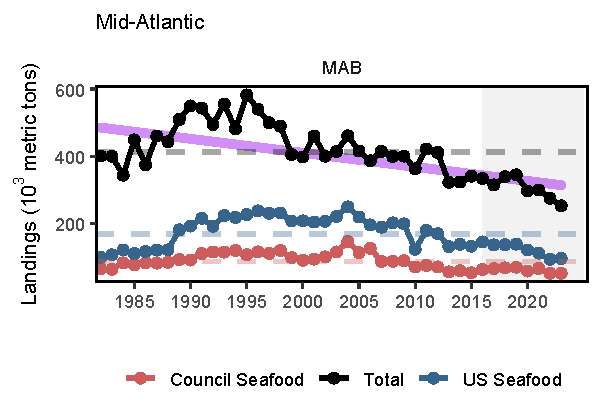
\includegraphics{midatlantic_files/figure-latex/total-landings-1} 

}

\caption{Total commercial landings (black), total U.S. seafood landings (blue), and Mid-Atlantic managed U.S. seafood landings (red), with significant decline (purple) in total landings.}\label{fig:total-landings}
\end{figure}

Commercial landings by guild include all species and all uses, and are reported as total for the guild and the MAFMC managed species within the \href{https://noaa-edab.github.io/catalog/species_groupings.html}{guild}. Landings of benthos have been below the long term average since 2010, primarily driven by surf clam and ocean quahog, with scallops now contributing to the decline as well. Total landings of planktivores is presenting a significant downward trend, primarily due to decreases in species not managed by the MAFMC (Atlantic herring and Atlantic menhaden; Fig. \ref{fig:comm-landings}).

\begin{figure}

{\centering 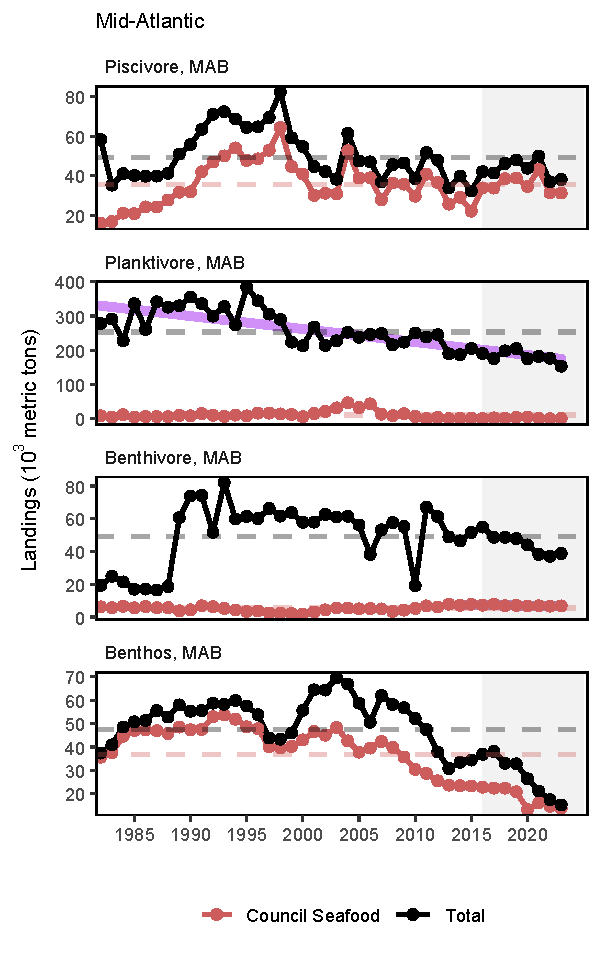
\includegraphics{midatlantic_files/figure-latex/comm-landings-1} 

}

\caption{Total commercial landings in the Mid-Atlantic Bight (black) and MAFMC-managed U.S seafood landings (red) by feeding guild, with significant declines (purple) in total planktivore landings.}\label{fig:comm-landings}
\end{figure}

\href{https://noaa-edab.github.io/catalog/community_climate_vulnerability.html}{Community Climate Change Risk indicators} have been developed to evaluate port specific landings and revenue risk in terms of commercial species climate vulnerability. The total climate vulnerability is a measure of to what degree a region's landings (or revenue) is dependent on species sensitive to different climate and environmental change factors including temperature and acidification. For ports combined across Mid-Atlantic states, the total climate vulnerability of landings ranged between moderate and high with a long term increase from 2000-2021 (Fig. \ref{fig:climatevul-land}).

\begin{figure}

{\centering 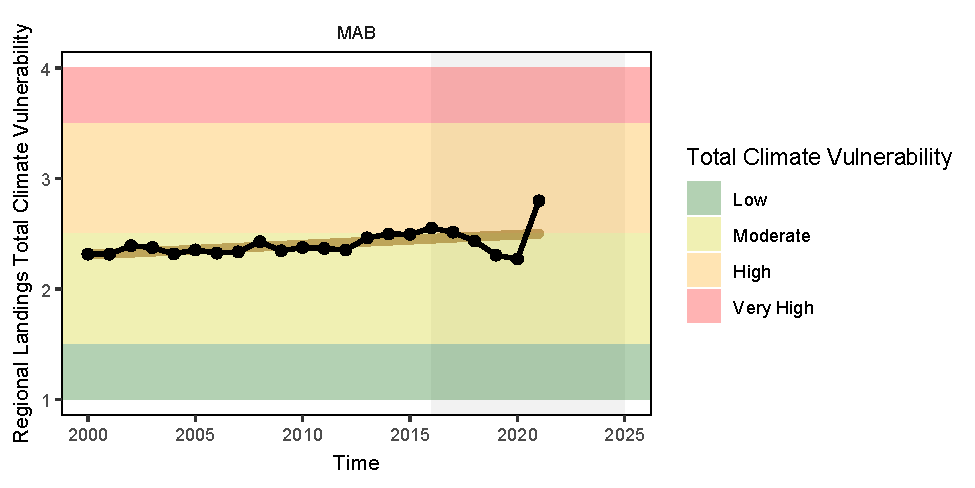
\includegraphics{midatlantic_files/figure-latex/climatevul-land-1} 

}

\caption{Mid-Atlantic region total climate vulnerability of commercial landings (sum of Mid-Atlantic port landings weighted by species climate vulnerability from Hare et al. 2016).}\label{fig:climatevul-land}
\end{figure}

Although total \href{https://noaa-edab.github.io/catalog/recdat.html}{recreational harvest} (fish presumed to be eaten) has increased from a historic low in 2018, there is a long-term decline in the Mid-Atlantic (Fig. \ref{fig:rec-landings}).

\begin{figure}

{\centering 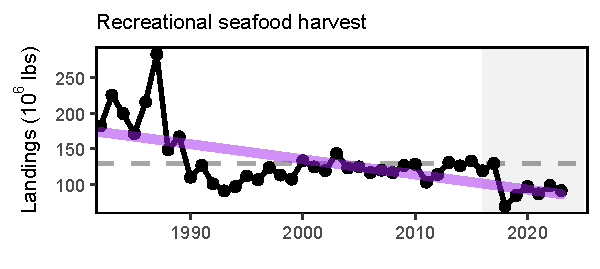
\includegraphics{midatlantic_files/figure-latex/rec-landings-1} 

}

\caption{Total recreational seafood harvest (millions of pounds, black, significant decrease, purple) in the Mid-Atlantic region.}\label{fig:rec-landings}
\end{figure}

\href{https://noaa-edab.github.io/catalog/rec_hms.html}{Recreational shark landings} have generally decreased for most shark groups through 2023 (Fig \ref{fig:rec-hms}). The recent low in pelagic shark landings is likely influenced by regulatory changes implemented in 2018 intended to rebuild shortfin mako stocks and comply with binding recommendations by the International Commission for the Conservation of Atlantic Tunas (ICCAT).

\begin{figure}

{\centering 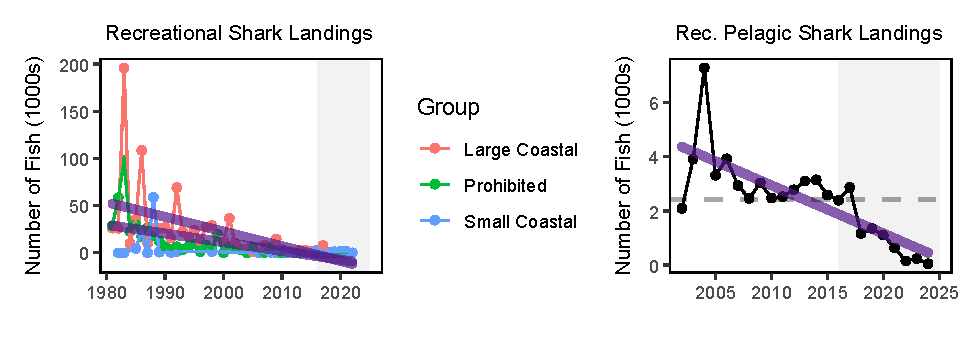
\includegraphics{midatlantic_files/figure-latex/rec-hms-1} 

}

\caption{Recreational shark landings from Marine Recreational Information Program (left) and Large Pelagics Survey (right) with declining trends (purple).}\label{fig:rec-hms}
\end{figure}

Aquaculture production is not yet included in total seafood landings. Available \href{https://noaa-edab.github.io/catalog/aquaculture.html}{aquaculture production} of oysters for a subset of Mid-Atlantic states indicates a decline in recent years.

\subsubsection{Implications}\label{implications}

Declining commercial (total and seafood) landings and recreational harvest can be driven by many interacting factors, including combinations of ecosystem and stock production, management actions, market conditions, and environmental change. While we cannot evaluate all possible drivers at present, here we evaluate the extent to which stock status, management, and system biomass trends may play a role.

\paragraph{Stock Status and Catch Limits}\label{stock-status-and-catch-limits}

Single species \href{https://noaa-edab.github.io/catalog/stock_status.html}{management objectives} (1. maintaining biomass above minimum thresholds and 2. maintaining fishing mortality below overfishing limits) are being met for all but three MAFMC-managed species (Fig. \ref{fig:stock-status}), though the status of six stocks is unknown (Table \ref{tab:unkstocks}).

\begin{figure}

{\centering 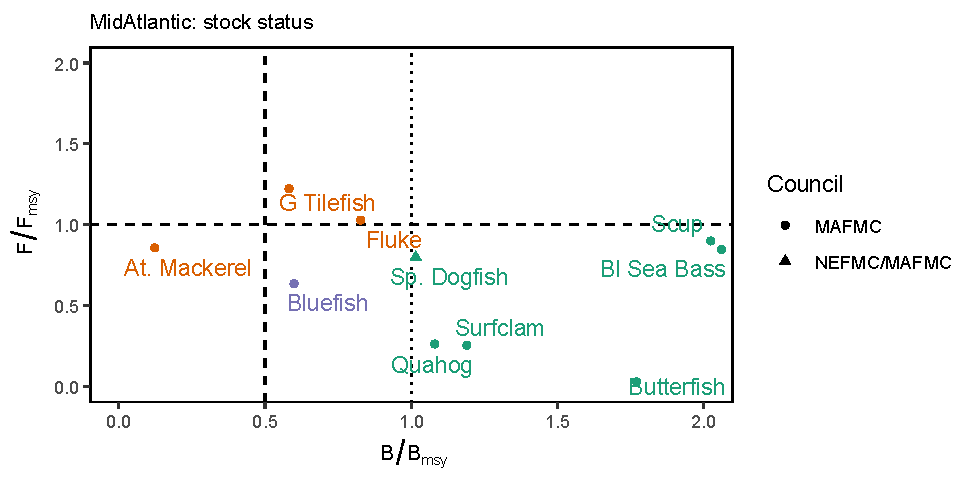
\includegraphics{midatlantic_files/figure-latex/stock-status-1} 

}

\caption{Summary of single species status for MAFMC and jointly federally managed stocks (Spiny dogfish and both Goosefish). The dotted vertical line is the target biomass reference point of $B_{MSY}$. The dashed lines are the management thresholds of one half $B_{MSY}$ (vertical) or $F_{MSY}$. (horizontal). Stocks in orange are below the biomass threshold (overfished) or have fishing mortality above the limit (subject to overfishing), so are not meeting objectives. Stocks in purple  are above the biomass threshold but below the biomass target with fishing mortality within the limit. Stocks in green are above the biomass target, with fishing mortality within the limit.}\label{fig:stock-status}
\end{figure}

\global\setlength{\Oldarrayrulewidth}{\arrayrulewidth}

\global\setlength{\Oldtabcolsep}{\tabcolsep}

\setlength{\tabcolsep}{2pt}

\renewcommand*{\arraystretch}{1.5}



\providecommand{\ascline}[3]{\noalign{\global\arrayrulewidth #1}\arrayrulecolor[HTML]{#2}\cline{#3}}

\begin{longtable}[c]{|p{3.29in}|p{0.70in}|p{0.72in}}

\caption{Unknown\ or\ partially\ known\ stock\ status\ for\ MAFMC\ and\ jointly\ managed\ species.}\label{tab:unkstocks}\\

\ascline{1.5pt}{666666}{1-3}

\multicolumn{1}{>{\raggedright}m{\dimexpr 3.29in+0\tabcolsep}}{\textcolor[HTML]{000000}{\fontsize{9}{9}\selectfont{Stock}}} & \multicolumn{1}{>{\raggedleft}m{\dimexpr 0.7in+0\tabcolsep}}{\textcolor[HTML]{000000}{\fontsize{9}{9}\selectfont{F/Fmsy}}} & \multicolumn{1}{>{\raggedleft}m{\dimexpr 0.72in+0\tabcolsep}}{\textcolor[HTML]{000000}{\fontsize{9}{9}\selectfont{B/Bmsy}}} \\

\ascline{1.5pt}{666666}{1-3}\endfirsthead \caption[]{Unknown\ or\ partially\ known\ stock\ status\ for\ MAFMC\ and\ jointly\ managed\ species.}\label{tab:unkstocks}\\

\ascline{1.5pt}{666666}{1-3}

\multicolumn{1}{>{\raggedright}m{\dimexpr 3.29in+0\tabcolsep}}{\textcolor[HTML]{000000}{\fontsize{9}{9}\selectfont{Stock}}} & \multicolumn{1}{>{\raggedleft}m{\dimexpr 0.7in+0\tabcolsep}}{\textcolor[HTML]{000000}{\fontsize{9}{9}\selectfont{F/Fmsy}}} & \multicolumn{1}{>{\raggedleft}m{\dimexpr 0.72in+0\tabcolsep}}{\textcolor[HTML]{000000}{\fontsize{9}{9}\selectfont{B/Bmsy}}} \\

\ascline{1.5pt}{666666}{1-3}\endhead



\multicolumn{1}{>{\raggedright}m{\dimexpr 3.29in+0\tabcolsep}}{\textcolor[HTML]{000000}{\fontsize{9}{9}\selectfont{Longfin\ inshore\ squid\ -\ Georges\ Bank\ /\ Cape\ Hatteras}}} & \multicolumn{1}{>{\raggedleft}m{\dimexpr 0.7in+0\tabcolsep}}{\textcolor[HTML]{000000}{\fontsize{9}{9}\selectfont{-}}} & \multicolumn{1}{>{\raggedleft}m{\dimexpr 0.72in+0\tabcolsep}}{\textcolor[HTML]{000000}{\fontsize{9}{9}\selectfont{2.873}}} \\





\multicolumn{1}{>{\raggedright}m{\dimexpr 3.29in+0\tabcolsep}}{\textcolor[HTML]{000000}{\fontsize{9}{9}\selectfont{Northern\ shortfin\ squid\ -\ Northwestern\ Atlantic\ Coast}}} & \multicolumn{1}{>{\raggedleft}m{\dimexpr 0.7in+0\tabcolsep}}{\textcolor[HTML]{000000}{\fontsize{9}{9}\selectfont{-}}} & \multicolumn{1}{>{\raggedleft}m{\dimexpr 0.72in+0\tabcolsep}}{\textcolor[HTML]{000000}{\fontsize{9}{9}\selectfont{-}}} \\





\multicolumn{1}{>{\raggedright}m{\dimexpr 3.29in+0\tabcolsep}}{\textcolor[HTML]{000000}{\fontsize{9}{9}\selectfont{Goosefish\ -\ Gulf\ of\ Maine\ /\ Northern\ Georges\ Bank}}} & \multicolumn{1}{>{\raggedleft}m{\dimexpr 0.7in+0\tabcolsep}}{\textcolor[HTML]{000000}{\fontsize{9}{9}\selectfont{-}}} & \multicolumn{1}{>{\raggedleft}m{\dimexpr 0.72in+0\tabcolsep}}{\textcolor[HTML]{000000}{\fontsize{9}{9}\selectfont{-}}} \\





\multicolumn{1}{>{\raggedright}m{\dimexpr 3.29in+0\tabcolsep}}{\textcolor[HTML]{000000}{\fontsize{9}{9}\selectfont{Goosefish\ -\ Southern\ Georges\ Bank\ /\ Mid-Atlantic}}} & \multicolumn{1}{>{\raggedleft}m{\dimexpr 0.7in+0\tabcolsep}}{\textcolor[HTML]{000000}{\fontsize{9}{9}\selectfont{-}}} & \multicolumn{1}{>{\raggedleft}m{\dimexpr 0.72in+0\tabcolsep}}{\textcolor[HTML]{000000}{\fontsize{9}{9}\selectfont{-}}} \\





\multicolumn{1}{>{\raggedright}m{\dimexpr 3.29in+0\tabcolsep}}{\textcolor[HTML]{000000}{\fontsize{9}{9}\selectfont{Blueline\ tilefish\ -\ Mid-Atlantic\ Coast}}} & \multicolumn{1}{>{\raggedleft}m{\dimexpr 0.7in+0\tabcolsep}}{\textcolor[HTML]{000000}{\fontsize{9}{9}\selectfont{-}}} & \multicolumn{1}{>{\raggedleft}m{\dimexpr 0.72in+0\tabcolsep}}{\textcolor[HTML]{000000}{\fontsize{9}{9}\selectfont{-}}} \\





\multicolumn{1}{>{\raggedright}m{\dimexpr 3.29in+0\tabcolsep}}{\textcolor[HTML]{000000}{\fontsize{9}{9}\selectfont{Chub\ mackerel\ -\ Atlantic}}} & \multicolumn{1}{>{\raggedleft}m{\dimexpr 0.7in+0\tabcolsep}}{\textcolor[HTML]{000000}{\fontsize{9}{9}\selectfont{-}}} & \multicolumn{1}{>{\raggedleft}m{\dimexpr 0.72in+0\tabcolsep}}{\textcolor[HTML]{000000}{\fontsize{9}{9}\selectfont{-}}} \\

\ascline{1.5pt}{666666}{1-3}



\end{longtable}



\arrayrulecolor[HTML]{000000}

\global\setlength{\arrayrulewidth}{\Oldarrayrulewidth}

\global\setlength{\tabcolsep}{\Oldtabcolsep}

\renewcommand*{\arraystretch}{1}

Stock status affects catch limits established by the Council, which in turn may affect landings trends. Summed across all MAFMC managed species, total Acceptable Biological Catch or Annual Catch Limits \href{https://noaa-edab.github.io/catalog/abc_acl.html}{(ABC or ACL)} have been relatively stable 2012-2023 (Fig. \ref{fig:abcacl-stacked}). The recent total ABC or ACL is lower relative to 2012-2013, with much of that decrease due to declining Atlantic mackerel ABC. This is true even with the addition of blueline tilefish management contributing an additional ABC to the total post-2017, due to that fishery's small relative size.

\begin{figure}

{\centering 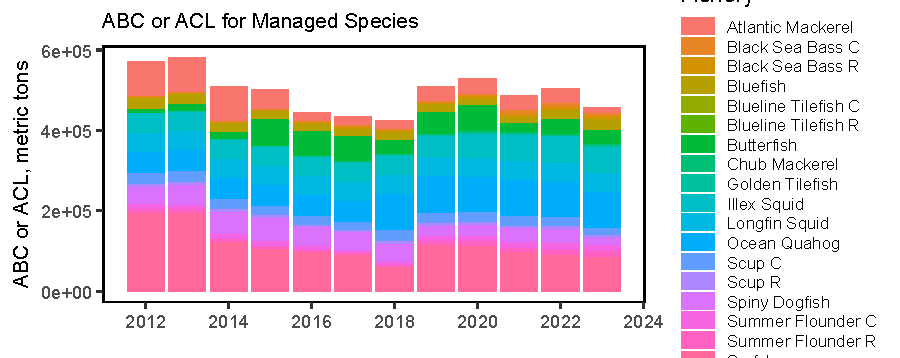
\includegraphics{midatlantic_files/figure-latex/abcacl-stacked-1} 

}

\caption{Sum of catch limits across all MAFMC managed commercial (C) and recreational (R) fisheries.}\label{fig:abcacl-stacked}
\end{figure}

Nevertheless, the percentage caught (landings and discards) for each stock's ABC/ACL suggests that these catch limits are not generally constraining as most species are well below the 1/1 ratio (Fig. \ref{fig:abcacl-catch}). Therefore, stock status and associated management constraints are unlikely to be driving decreased landings for the majority of species.

\begin{figure}

{\centering 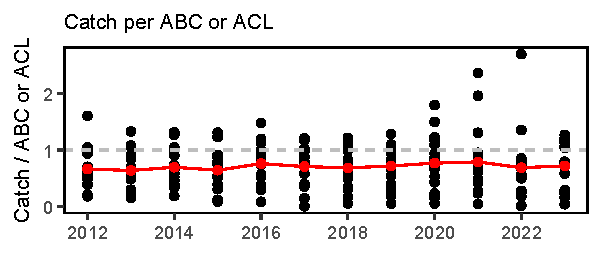
\includegraphics{midatlantic_files/figure-latex/abcacl-catch-1} 

}

\caption{Catch divided by ABC/ACL for MAFMC managed fisheries. High points are recreational black sea bass (up to 2021) and scup (2022). Red line indicates the median ratio across all fisheries.}\label{fig:abcacl-catch}
\end{figure}

\paragraph{System Biomass}\label{system-biomass}

Although \href{https://noaa-edab.github.io/catalog/aggregate_biomass.html}{aggregate biomass} trends derived from scientific resource surveys are mostly stable in the MAB, spring piscivores, fall benthivores, and fall benthos show long-term increases (Fig. \ref{fig:nefsc-biomass-mab}). While managed species make up varying proportions of aggregate biomass, trends in landings are not mirroring shifts in the overall trophic structure of survey-sampled fish and invertebrates. Therefore, major shifts in feeding guilds or ecosystem trophic structure are unlikely to be driving the decline in landings.

\begin{figure}

{\centering 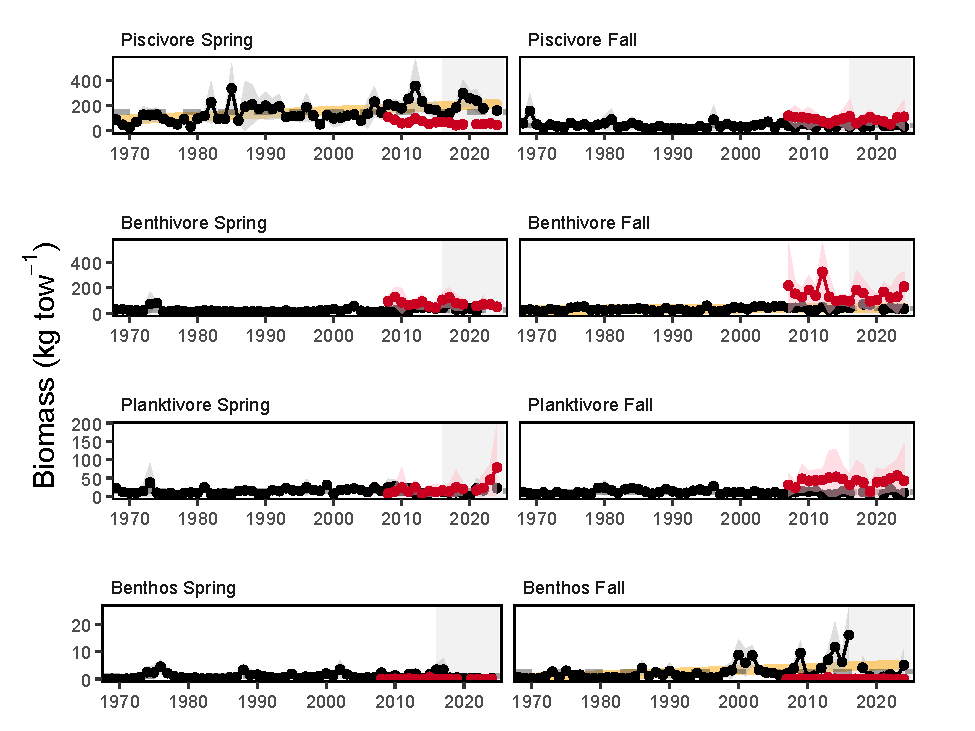
\includegraphics{midatlantic_files/figure-latex/nefsc-biomass-mab-1} 

}

\caption{Spring (left) and fall (right) surveyed biomass in the Mid-Atlantic Bight. Data from the NEFSC Bottom Trawl Survey are shown in black, with the nearshore NEAMAP survey shown in red. Significant increases (orange lines) are present for spring piscivore and fall benthivore and benthos biomass. The shaded area around each annual mean represents 2 standard deviations from the mean.}\label{fig:nefsc-biomass-mab}
\end{figure}

\paragraph{Effect on Seafood Production}\label{effect-on-seafood-production}

Stock status is above the minimum threshold for all but one stock, and aggregate biomass trends appear stable or increasing, so the decline in managed commercial seafood landings is most likely driven by market dynamics affecting the landings of surfclams and ocean quahogs, as landings have been below quotas for these species. In addition, regional availability of scallops has contributed to the decline of benthos landings not managed by the MAFMC, with some of the most productive grounds closed through 2023 due to rotational management. The long term decline in total planktivore landings, and total landings, is largely driven by Atlantic menhaden fishery dynamics, including a consolidation of processors leading to reduced fishing capacity between the 1990s and mid-2000s.

The distribution of surfclams and ocean quahogs is changing, resulting in areas with overlapping distributions and increased mixed landings. Given the regulations governing mixed landings, this could have become problematic and the Council recently took final action to address this issue.

The decline in recreational seafood harvest stems from other drivers. Some of the decline, such as that for recreational shark landings, is driven by management intended to reduce fishing mortality on mako sharks. However, NOAA Fisheries' Marine Recreational Information Program survey methodology was updated in 2018, so it is unclear whether the lower than average landings for species other than sharks since 2018 are driven by changes in fishing behavior or the change in the survey methodology. Nevertheless, the recreational harvest appears to be stabilizing at a lower level than historical estimates.

Other environmental changes require monitoring as they may become important drivers of commercial and recreational landings in the future. Overall, landings from Mid-Atlantic ports depend on species with moderate climate vulnerability, and the proportion of landings with higher vulnerability has increased over time. We note that individual stocks will respond differently to these drivers, and fisheries and communities rely on different combinations of stocks:

\begin{itemize}
\tightlist
\item
  Climate is trending into uncharted territory. Globally, 2024 was the warmest year on record (see \hyperref[highlights]{2024 Highlights section}).
\item
  Stocks are shifting their distributions, moving towards the northeast and into deeper waters throughout the Northeast US Large Marine Ecosystem (see \hyperref[climate-and-ecosystem-change]{Climate Risks section}).
\item
  Some ecosystem composition and production changes have been observed (see \hyperref[stability]{Stability section}).
\item
  Some fishing communities are affected by socioeconomic vulnerabilities (see \hyperref[community-social-and-climate-vulnerability]{Community Social and Climate Vulnerability section}).
\end{itemize}

\begin{verbatim}
## [1] "Ending 01_seafood_production_midatlantic.Rmd"
\end{verbatim}

\subsection{Commercial Profits}\label{commercial-profits}

\begin{verbatim}
## [1] "Beginning 02_commercial_profits_midatlantic.Rmd"
\end{verbatim}

\subsubsection{Indicators: revenue (a proxy for profits)}\label{indicators-revenue-a-proxy-for-profits}

Total \href{https://noaa-edab.github.io/catalog/comdat.html}{commercial revenue} and MAFMC managed species revenue within the Mid-Atlantic Bight have declined over the past 20-30 years. In 2023, total revenue was at an all-time low, and revenue from MAFMC managed species was near an all-time low (Fig. \ref{fig:comm-revenue}).

Revenue earned by harvesting resources is a function of both the quantity landed of each species and the prices paid for landings. Beyond monitoring yearly changes in revenue, it is even more valuable to determine what drives these changes: harvest levels, the mix of species landed, price changes, or a combination of these. The \href{https://noaa-edab.github.io/catalog/bennet.html}{Bennet Indicator} decomposes revenue change into two parts, one driven by changing quantities (volumes), and a second driven by changing prices. All changes are in relation to a base year (1982). The 1982 base year was selected because that is the first year the relevant data is available and it also allows for an extended period of time in which to evaluate market trends and dynamics.

In the Mid-Atlantic region revenues were above the 1982 baseline for all years in the series until 2022 and 2023 (Fig. \ref{fig:bennet}). In 2023, lower revenue was driven primarily by both lower quantities of benthos landed, and lower prices of benthos, benthivores, and planktivores. The lower benthos prices are a departure from past years, which saw benthos prices contributing positively to revenue changes since the early 2000's. (Fig. \ref{fig:bennet-all}).

\begin{figure}

{\centering 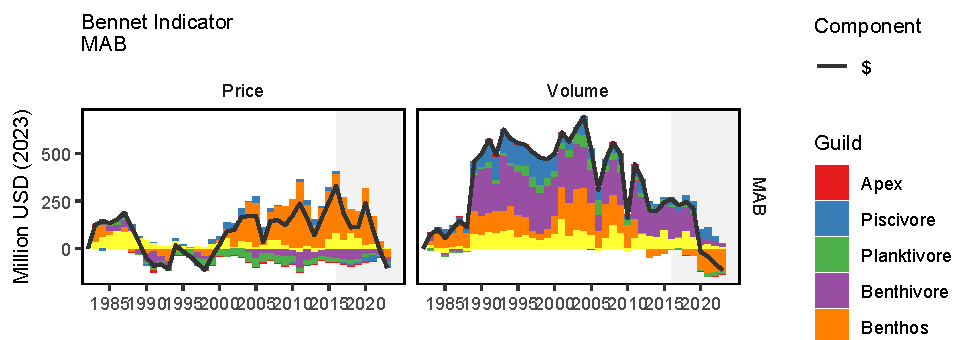
\includegraphics{midatlantic_files/figure-latex/bennet-all-1} 

}

\caption{Total price and volume indicators in 2023 dollars (black) for commercial landings, and individual guild contributions to each indicator, in the Mid-Atlantic Bight.}\label{fig:bennet-all}
\end{figure}

For ports combined across Mid-Atlantic states, \href{https://noaa-edab.github.io/catalog/community_climate_vulnerability.html}{total climate vulnerability} of revenue ranged from high to very high from 2000-2021, with no long-term trend. This suggests that Mid-Atlantic port commercial fishing revenue has been highly reliant on climate-sensitive species for most of the period since 2000 (Fig. \ref{fig:climatevul-rev}).

\begin{figure}

{\centering 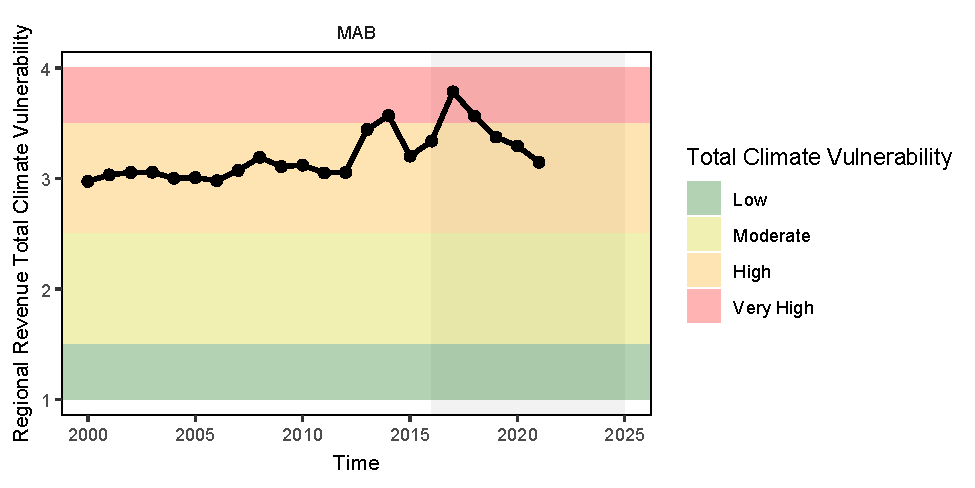
\includegraphics{midatlantic_files/figure-latex/climatevul-rev-1} 

}

\caption{Mid-Atlantic region total climate vulnerability of commercial revenue (sum of Mid-Atlantic port revenue weighted by species climate vulnerability from Hare et al. 2016).}\label{fig:climatevul-rev}
\end{figure}

\subsubsection{Implications}\label{implications-1}

Although the Mid-Atlantic region shows declining revenue since 2016, inflation-adjusted revenue from harvested species was still greater than 1982 levels until the past two years. In a similar manner to seafood landings, the results here are driven in large part by market dynamics affecting the landings of surfclams and ocean quahogs, as landings have been below quotas for these species, as well as lower quotas and prices for Atlantic scallops. The declining benthos category since 2012 may be partially caused by decreases in surfclam and ocean quahogs in the southern part of their range as harvest have shifted northward. Changes in other indicators, particularly those driving landings and those related to climate change, require monitoring as they may become important drivers of revenue in the future; for example:

\begin{itemize}
\tightlist
\item
  Surfclams, ocean quahogs, and scallops are sensitive to warming ocean temperatures and ocean acidification, as reflected in the high climate vulnerability of total landings from from Mid-Atlantic ports.
\item
  Multiple stressors including \href{https://noaa-edab.github.io/catalog/bottom_temp_insitu.html}{warming} and \href{https://noaa-edab.github.io/catalog/ocean_acidification}{ocean acidification} are interacting in Mid-Atlantic shellfish habitats.
\end{itemize}

\begin{verbatim}
## [1] "Ending 02_commercial_profits_midatlantic.Rmd"
\end{verbatim}

\subsection{Recreational Opportunities}\label{recreational-opportunities}

\begin{verbatim}
## [1] "Beginning 03_recreational_opportunities_midatlantic.Rmd"
\end{verbatim}

\subsubsection{Indicators: Angler trips, fleet diversity}\label{indicators-angler-trips-fleet-diversity}

\href{https://noaa-edab.github.io/catalog/recdat.html}{Recreational effort} (angler trips) in 2023 continues to be above the long-term average (Fig. \ref{fig:rec-op}). in the MAB. However, recreational fleet diversity (i.e., effort by shoreside, private boat, and for-hire anglers) has declined over the long term (Fig. \ref{fig:rec-div}).

\begin{figure}

{\centering 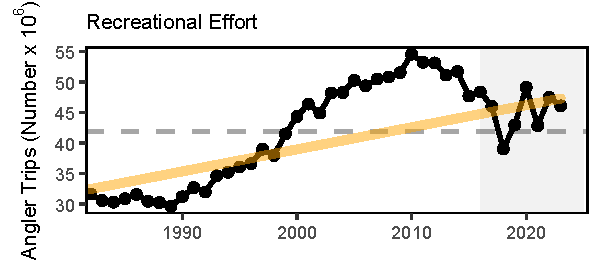
\includegraphics{midatlantic_files/figure-latex/rec-op-1} 

}

\caption{Recreational effort (number of trips, black) in the Mid-Atlantic, with significant increase (orange line).}\label{fig:rec-op}
\end{figure}

\begin{figure}

{\centering 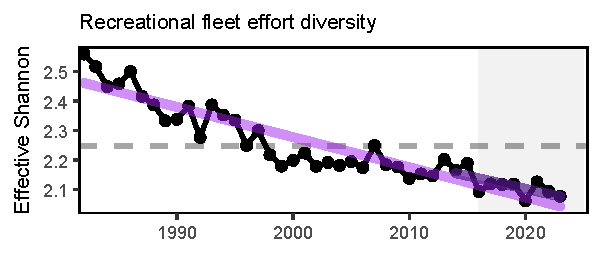
\includegraphics{midatlantic_files/figure-latex/rec-div-1} 

}

\caption{Recreational fleet effort diversity (black) in the Mid-Atlantic, with significant decrease (purple line).}\label{fig:rec-div}
\end{figure}

\subsubsection{Implications}\label{implications-2}

While the overall number of recreational opportunities in the MAB is above the long-term average, the continuing decline in recreational fleet effort diversity suggests a potentially reduced range of recreational fishing options.

The downward effort diversity trend is driven by party/charter contraction (down from 2.2\% in 2021 to 1.3\% of trips in 2023), and a shift toward shorebased angling, which currently makes up 60\% of all angler trips. Effort in private boats has remained relatively stable from 2022 values.

Changes in recreational fleet diversity can be considered when managers seek options to maintain recreational opportunities. Shore anglers will have access to different species than vessel-based anglers, and when the same species is accessible both from shore and from a vessel, shore anglers typically have access to smaller individuals. Many states have developed shore-based regulations where the minimum size is lower than in other areas and sectors to maintain opportunities in the shore angling sector. MAFMC is currently considering recreational sector separation which might establish different options for managing the for-hire sector from other modes.

\begin{verbatim}
## [1] "Ending 03_recreational_opportunities_midatlantic.Rmd"
\end{verbatim}

\subsection{Stability}\label{stability}

\begin{verbatim}
## [1] "Beginning 04_stability_midatlantic.Rmd"
\end{verbatim}

\subsubsection{Indicators: fishery fleet and catch diversity, ecological component diversity}\label{indicators-fishery-fleet-and-catch-diversity-ecological-component-diversity}

While there are many potential metrics of stability, we use diversity indices to evaluate overall stability in fisheries and ecosystems. In general, diversity that remains constant over time suggests a similar capacity to respond to change over time. A significant change in diversity over time does not necessarily indicate a problem or an improvement, but does indicate a need for further investigation. We examine diversity in commercial fleet and species catch, recreational species catch (with fleet effort diversity discussed above), zooplankton, adult fishes, and fish traits (e.g.~size and fecundity).

\paragraph{Fishery Stability}\label{fishery-stability}

Several \href{https://noaa-edab.github.io/catalog/commercial_div.html}{diversity} estimates are used to evaluate stability for fleets landing federally managed species, and species landed by commercial vessels with Mid-Atlantic permits. Commercial fishery fleet count has declined while fleet revenue diversity has been stable over time in the MAB, with no trend identified, but current values are above the long-term average (Fig. \ref{fig:comm-div-fleet}).

\begin{figure}

{\centering 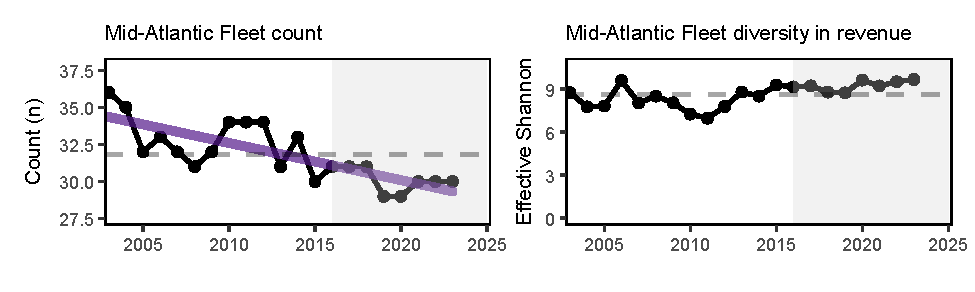
\includegraphics{midatlantic_files/figure-latex/comm-div-fleet-1} 

}

\caption{Commercial fleet count (left) and fleet diversity in revenue (right) in the Mid-Atlantic (black) with significant decline in fleet count (purple line).}\label{fig:comm-div-fleet}
\end{figure}

This indicates different commercial fleet composition but similar diversity in species targeting opportunities over time, for those fleets continuing to fish (Fig. \ref{fig:commercial-div-species-div}). Of note is that the current lack of vessel data available for surf clam and ocean quahog prior to 2003 precludes the assessment of longer term dynamics with these indicators.

\begin{figure}

{\centering 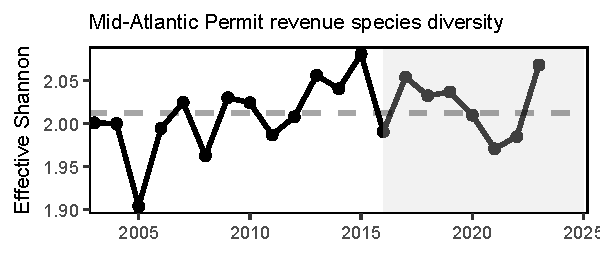
\includegraphics{midatlantic_files/figure-latex/commercial-div-species-div-1} 

}

\caption{Species revenue diversity in the Mid Atlantic.}\label{fig:commercial-div-species-div}
\end{figure}

As noted \hyperref[recreational-opportunities]{above}, \href{https://noaa-edab.github.io/catalog/recdat.html}{recreational fleet effort diversity} is declining (Fig. \ref{fig:rec-div}), suggesting a shift in recreational fishing opportunities. However, recreational species catch diversity has no long term trend so is considered stable, and has been at or above the long term average since 2016 (Fig. \ref{fig:recdat-div-catch}).

\begin{figure}

{\centering 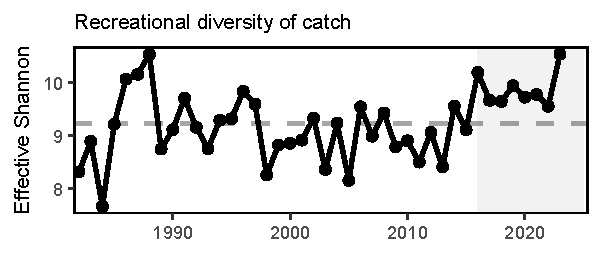
\includegraphics{midatlantic_files/figure-latex/recdat-div-catch-1} 

}

\caption{Diversity of recreational catch in the Mid Atlantic.}\label{fig:recdat-div-catch}
\end{figure}

\paragraph{Ecological Stability}\label{ecological-stability}

Ecological diversity indices show mixed trends. Total annual \href{https://noaa-edab.github.io/catalog/chl_pp.html}{primary production} is a measure of the total amount of carbon (i.e.~energy ) produced by phytoplankton per year. Total primary production in the Mid Atlantic Bight has no clear trend (Fig. \ref{fig:totpp}), suggesting stability in energy at the base of the food web.

\begin{figure}

{\centering 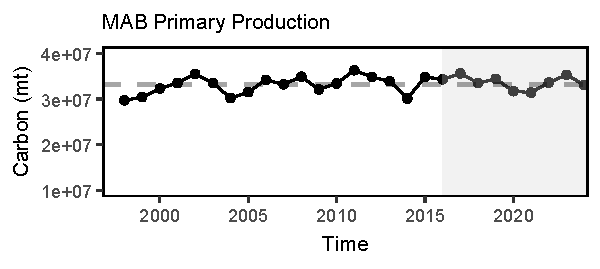
\includegraphics{midatlantic_files/figure-latex/totpp-1} 

}

\caption{Total areal annual primary production for the MAB. The dashed line represents the long-term (1998-2024) annual mean.}\label{fig:totpp}
\end{figure}

\href{https://noaa-edab.github.io/catalog/zoo_diversity.html}{Zooplankton diversity} is increasing in the MAB (Fig. \ref{fig:zoo-diversity}), while \href{https://noaa-edab.github.io/catalog/exp_n.html}{adult fish diversity}, the expected number of species in a standard number of individuals sampled from the NEFSC bottom trawl survey, appears stable over time, with current values within one standard deviation from most historic estimates (Fig. \ref{fig:exp-n}).

\begin{figure}

{\centering 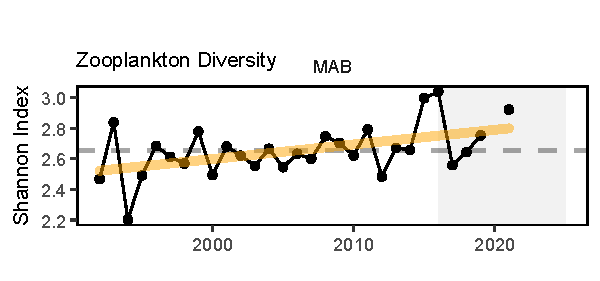
\includegraphics{midatlantic_files/figure-latex/zoo-diversity-1} 

}

\caption{Zooplankton diversity in the Mid-Atlantic Bight, Shannon diversity index (black) with significant increase (orange line).}\label{fig:zoo-diversity}
\end{figure}

\begin{figure}

{\centering 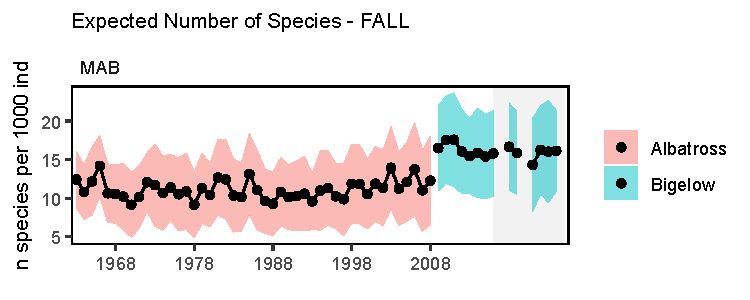
\includegraphics{midatlantic_files/figure-latex/exp-n-1} 

}

\caption{Adult fish diversity in the Mid-Atlantic Bight, based on expected number of species. Results from survey vessels Albatross and Bigelow are reported separately due to catchability differences.}\label{fig:exp-n}
\end{figure}

\href{https://noaa-edab.github.io/catalog/finfish_traits.html}{Functional traits}, such as length at maturity, maximum body size, or fecundity, can synthesize change across complex, diverse communities. Monitoring changes in functional trait distributions for the fish community can provide a means of assessing ecosystem-scale resilience. There is evidence of long term change in trait distributions in the MAB (Fig. \ref{fig:traits}). The spring finfish community in the MAB is showing long-term shifts towards slower life history strategies with higher length and maturity and lower fecundity. In contrast, the fall MAB finfish community has shifted towards decreased length at maturity, smaller offspring size, and lower trophic level indicative of faster life histories.

\begin{figure}

{\centering 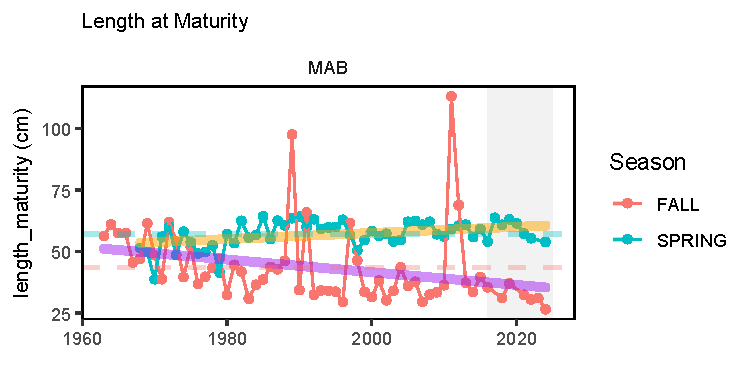
\includegraphics{midatlantic_files/figure-latex/traits-1} 

}

\caption{Fish community functional traits in the Mid Atlantic Bight based on Fall (red) and Spring (blue) survey data. Length at maturity for the full finfish community has increased in spring (orange line), but decreased in fall (purple lines)}\label{fig:traits}
\end{figure}

\subsubsection{Implications}\label{implications-3}

Fleet diversity indices are used by the MAFMC in their EAFM risk assessment to evaluate stability objectives as well as risks to fishery resilience and maintaining equity in access to fishery resources. Instability in the commercial fleet count metric suggests potentially lower capacity to respond to the current range of fishing opportunities. Commercial species permit revenue diversity is relatively stable but comparisons are limited by missing clam fishery data prior to 2003.

Declining recreational fleet effort diversity, as noted above, indicates that the party/charter boat sector continues to contract, with shoreside angling becoming more important as a percentage of recreational angler trips. Stability in recreational species catch diversity has been maintained by a different set of species over time. A recent increase in Atlantic States Marine Fisheries Commission (ASMFC) and South Atlantic Fishery Management Council (SAFMC) managed species in recreational catch is helping to maintain diversity in the same range that MAFMC and New England Fishery Management Council (NEFMC) managed species supported in the 1990s. These changes in effort and species trends may necessitate new or changing management considerations to ensure effective tools and opportunities are in place to support recreational fisheries.

Production at the base of the food web is variable, but stable over time. Stable adult fish diversity indicates the same overall number and evenness over time, but doesn't rule out species substitutions (e.g., warm-water replacing cold-water).

There was evidence for long term change in finfish trait distributions in the mid-Atlantic Bight, with spring and fall communities showing shifts in different directions. This suggests instability in seasonal dominance of fish with faster or slower life histories.

In the MAB, existing diversity indicators suggest some instability in the fisheries and ecosystem components examined. In addition, declining recreational fleet diversity suggests a potential loss in the range of recreational fishing opportunities. Increasing zooplankton diversity (due to increases in abundance of several taxa and stable or declining dominance of an important copepod species) suggests a shift in the zooplankton community that warrants continued monitoring to determine if managed species are affected. The species revenue diversity in commercial landings also warrants continued attention given its relatively low index value indicating average reliance on a small number of species for revenue.

\begin{verbatim}
## [1] "Ending 04_stability_midatlantic.Rmd"
\end{verbatim}

\subsection{Community Social and Climate Vulnerability}\label{community-social-and-climate-vulnerability}

Providing for sustained participation of fishing communities, and avoiding adverse economic impacts to fishing communities are objectives of fishery management. We report the top communities most engaged in commercial and recreational fisheries and the degree to which these communities may be vulnerable to change based on their socioeconomic conditions using data for the most recent available year (2022).

Coastal fishing communities worldwide have or are likely to experience social, economic, and cultural impacts from climate change, both negative (e.g., loss of infrastructure, fish stock decline) and positive (e.g., increased abundance of valuable species). Changes in marine fisheries as a consequence of climate change will require adaptation by coastal fishing communities and fisheries managers alike. The Community Climate Change Risk Indicators were developed to help examine trends in climate change vulnerability in U.S. coastal fishing communities in the Northeast Region using indicators developed to understand fishing community level risk to climate change as based on species dependency.

\begin{verbatim}
## [1] "Beginning 05_csvi_midatlantic.Rmd"
\end{verbatim}

\subsubsection{Indicators: Fishing Engagement and Community Social Vulnerability}\label{indicators-fishing-engagement-and-community-social-vulnerability}

The \href{https://noaa-edab.github.io/catalog/engagement.html}{engagement} indices demonstrate the importance of commercial and recreational fishing to a given community relative to other coastal communities in a region. Social vulnerability indicators measure social factors that shape a community's ability to adapt to change. For this report, we focus on top communities with the highest engagement scores, the top communities with the highest population relative engagement scores, and on three socio-demographic indicators within the CSVI toolset (poverty, personal disruption, population composition).

In 2022, Cape May, NJ; Reedville, VA; and Montauk, NY were the most engaged commercial fishing communities. Barnegat Light, NJ is much more engaged in commercial fishing relative to its population size when compared to other communities in the Mid-Atlantic (Fig.\ref{fig:commercial-engagement-1}). Cape May, NJ also ranked medium on the population composition index (calculated based on proportions of non-white, non-English speaking, and younger populations) and Atlantic City, NJ ranked high for all socio-demographic indicators suggesting that this important commercial fishing community may be more vulnerable to change in the future (Table \ref{tab:comvultab}).

Manteo, Vandemere, and Hobuken, NC are no longer listed as top ten recreational communities, replaced by Cape May and Barnegat Light, NJ; Orient, NY; Topsail Beach, Avon and Rodanthe, NC (Fig.\ref{fig:recreational-engagement-1}).

\begin{figure}

{\centering 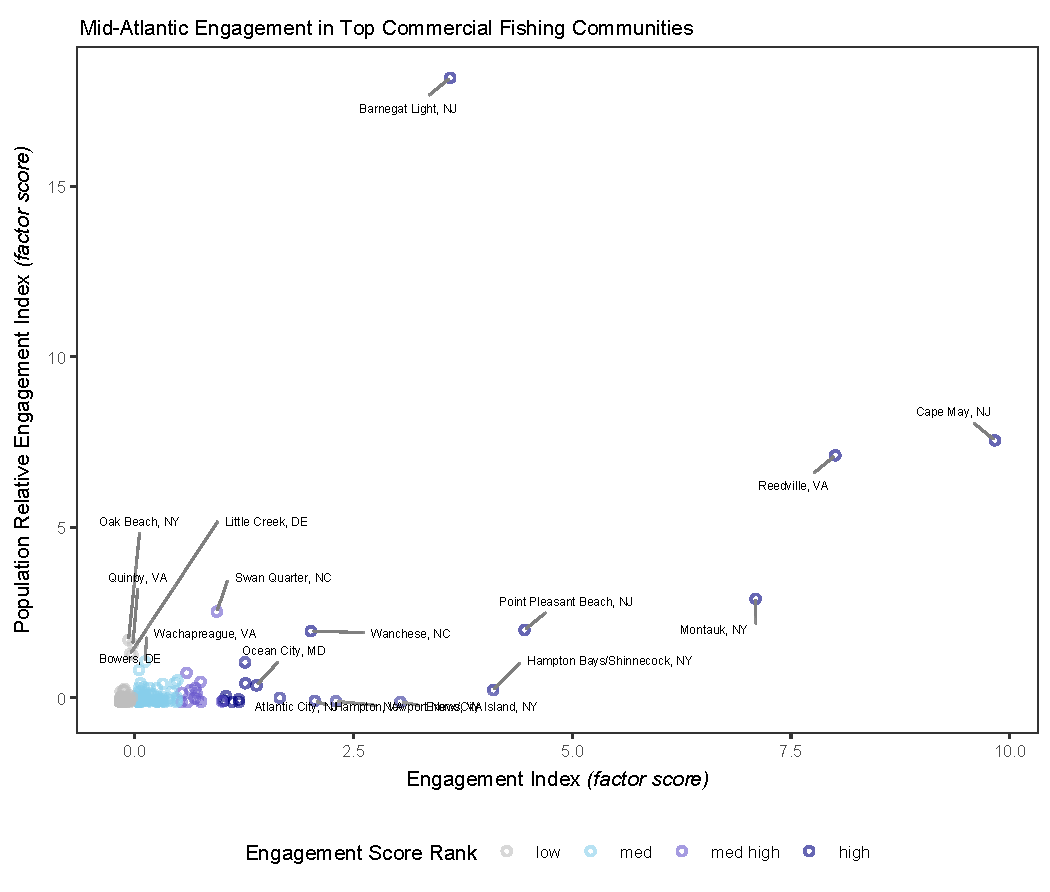
\includegraphics{midatlantic_files/figure-latex/commercial-engagement-1} 

}

\caption{Commercial engagement and population relative engagement, with labels for the top commercially engaged fishing communities in the Mid-Atlantic. *Due to changes in data infrastructure, data from Reedville, VA was combined with data from ‘Other VA' and 'Other Northumberland’.}\label{fig:commercial-engagement}
\end{figure}

\global\setlength{\Oldarrayrulewidth}{\arrayrulewidth}

\global\setlength{\Oldtabcolsep}{\tabcolsep}

\setlength{\tabcolsep}{2pt}

\renewcommand*{\arraystretch}{1.5}



\providecommand{\ascline}[3]{\noalign{\global\arrayrulewidth #1}\arrayrulecolor[HTML]{#2}\cline{#3}}

\begin{longtable}[c]{|p{2.03in}|p{1.38in}|p{1.61in}|p{0.71in}}

\caption{Socio-demographic\ indicator\ rankings\ (ranging\ from\ low\ =\ low\ vulnerability\ to\ high\ =\ high\ vulnerability)\ for\ Mid-Atlantic\ communities\ most\ engaged\ in\ commercial\ fishing,\ 2022.\ Blank\ spaces\ indicate\ no\ data\ available.}\label{tab:comvultab}\\

\ascline{1.5pt}{666666}{1-4}

\multicolumn{1}{>{\raggedright}m{\dimexpr 2.03in+0\tabcolsep}}{\textcolor[HTML]{000000}{\fontsize{9}{9}\selectfont{Community}}} & \multicolumn{1}{>{\raggedright}m{\dimexpr 1.38in+0\tabcolsep}}{\textcolor[HTML]{000000}{\fontsize{9}{9}\selectfont{Personal\ Disruption}}} & \multicolumn{1}{>{\raggedright}m{\dimexpr 1.61in+0\tabcolsep}}{\textcolor[HTML]{000000}{\fontsize{9}{9}\selectfont{Population\ Composition}}} & \multicolumn{1}{>{\raggedright}m{\dimexpr 0.71in+0\tabcolsep}}{\textcolor[HTML]{000000}{\fontsize{9}{9}\selectfont{Poverty}}} \\

\ascline{1.5pt}{666666}{1-4}\endfirsthead \caption[]{Socio-demographic\ indicator\ rankings\ (ranging\ from\ low\ =\ low\ vulnerability\ to\ high\ =\ high\ vulnerability)\ for\ Mid-Atlantic\ communities\ most\ engaged\ in\ commercial\ fishing,\ 2022.\ Blank\ spaces\ indicate\ no\ data\ available.}\label{tab:comvultab}\\

\ascline{1.5pt}{666666}{1-4}

\multicolumn{1}{>{\raggedright}m{\dimexpr 2.03in+0\tabcolsep}}{\textcolor[HTML]{000000}{\fontsize{9}{9}\selectfont{Community}}} & \multicolumn{1}{>{\raggedright}m{\dimexpr 1.38in+0\tabcolsep}}{\textcolor[HTML]{000000}{\fontsize{9}{9}\selectfont{Personal\ Disruption}}} & \multicolumn{1}{>{\raggedright}m{\dimexpr 1.61in+0\tabcolsep}}{\textcolor[HTML]{000000}{\fontsize{9}{9}\selectfont{Population\ Composition}}} & \multicolumn{1}{>{\raggedright}m{\dimexpr 0.71in+0\tabcolsep}}{\textcolor[HTML]{000000}{\fontsize{9}{9}\selectfont{Poverty}}} \\

\ascline{1.5pt}{666666}{1-4}\endhead



\multicolumn{1}{>{\raggedright}m{\dimexpr 2.03in+0\tabcolsep}}{\textcolor[HTML]{000000}{\fontsize{9}{9}\selectfont{Cape\ May,\ NJ}}} & \multicolumn{1}{>{\raggedright}m{\dimexpr 1.38in+0\tabcolsep}}{\textcolor[HTML]{000000}{\fontsize{9}{9}\selectfont{low}}} & \multicolumn{1}{>{\raggedright}m{\dimexpr 1.61in+0\tabcolsep}}{\textcolor[HTML]{000000}{\fontsize{9}{9}\selectfont{med}}} & \multicolumn{1}{>{\raggedright}m{\dimexpr 0.71in+0\tabcolsep}}{\textcolor[HTML]{000000}{\fontsize{9}{9}\selectfont{low}}} \\





\multicolumn{1}{>{\raggedright}m{\dimexpr 2.03in+0\tabcolsep}}{\textcolor[HTML]{000000}{\fontsize{9}{9}\selectfont{Reedville,\ VA}}} & \multicolumn{1}{>{\raggedright}m{\dimexpr 1.38in+0\tabcolsep}}{\textcolor[HTML]{000000}{\fontsize{9}{9}\selectfont{low}}} & \multicolumn{1}{>{\raggedright}m{\dimexpr 1.61in+0\tabcolsep}}{\textcolor[HTML]{000000}{\fontsize{9}{9}\selectfont{low}}} & \multicolumn{1}{>{\raggedright}m{\dimexpr 0.71in+0\tabcolsep}}{\textcolor[HTML]{000000}{\fontsize{9}{9}\selectfont{low}}} \\





\multicolumn{1}{>{\raggedright}m{\dimexpr 2.03in+0\tabcolsep}}{\textcolor[HTML]{000000}{\fontsize{9}{9}\selectfont{Montauk,\ NY}}} & \multicolumn{1}{>{\raggedright}m{\dimexpr 1.38in+0\tabcolsep}}{\textcolor[HTML]{000000}{\fontsize{9}{9}\selectfont{low}}} & \multicolumn{1}{>{\raggedright}m{\dimexpr 1.61in+0\tabcolsep}}{\textcolor[HTML]{000000}{\fontsize{9}{9}\selectfont{low}}} & \multicolumn{1}{>{\raggedright}m{\dimexpr 0.71in+0\tabcolsep}}{\textcolor[HTML]{000000}{\fontsize{9}{9}\selectfont{low}}} \\





\multicolumn{1}{>{\raggedright}m{\dimexpr 2.03in+0\tabcolsep}}{\textcolor[HTML]{000000}{\fontsize{9}{9}\selectfont{Point\ Pleasant\ Beach,\ NJ}}} & \multicolumn{1}{>{\raggedright}m{\dimexpr 1.38in+0\tabcolsep}}{\textcolor[HTML]{000000}{\fontsize{9}{9}\selectfont{med}}} & \multicolumn{1}{>{\raggedright}m{\dimexpr 1.61in+0\tabcolsep}}{\textcolor[HTML]{000000}{\fontsize{9}{9}\selectfont{low}}} & \multicolumn{1}{>{\raggedright}m{\dimexpr 0.71in+0\tabcolsep}}{\textcolor[HTML]{000000}{\fontsize{9}{9}\selectfont{low}}} \\





\multicolumn{1}{>{\raggedright}m{\dimexpr 2.03in+0\tabcolsep}}{\textcolor[HTML]{000000}{\fontsize{9}{9}\selectfont{Hampton\ Bays/Shinnecock,\ NY}}} & \multicolumn{1}{>{\raggedright}m{\dimexpr 1.38in+0\tabcolsep}}{\textcolor[HTML]{000000}{\fontsize{9}{9}\selectfont{low}}} & \multicolumn{1}{>{\raggedright}m{\dimexpr 1.61in+0\tabcolsep}}{\textcolor[HTML]{000000}{\fontsize{9}{9}\selectfont{high}}} & \multicolumn{1}{>{\raggedright}m{\dimexpr 0.71in+0\tabcolsep}}{\textcolor[HTML]{000000}{\fontsize{9}{9}\selectfont{low}}} \\





\multicolumn{1}{>{\raggedright}m{\dimexpr 2.03in+0\tabcolsep}}{\textcolor[HTML]{000000}{\fontsize{9}{9}\selectfont{Barnegat\ Light,\ NJ}}} & \multicolumn{1}{>{\raggedright}m{\dimexpr 1.38in+0\tabcolsep}}{\textcolor[HTML]{000000}{\fontsize{9}{9}\selectfont{low}}} & \multicolumn{1}{>{\raggedright}m{\dimexpr 1.61in+0\tabcolsep}}{\textcolor[HTML]{000000}{\fontsize{9}{9}\selectfont{low}}} & \multicolumn{1}{>{\raggedright}m{\dimexpr 0.71in+0\tabcolsep}}{\textcolor[HTML]{000000}{\fontsize{9}{9}\selectfont{low}}} \\





\multicolumn{1}{>{\raggedright}m{\dimexpr 2.03in+0\tabcolsep}}{\textcolor[HTML]{000000}{\fontsize{9}{9}\selectfont{Bronx/City\ Island,\ NY}}} & \multicolumn{1}{>{\raggedright}m{\dimexpr 1.38in+0\tabcolsep}}{\textcolor[HTML]{000000}{\fontsize{9}{9}\selectfont{high}}} & \multicolumn{1}{>{\raggedright}m{\dimexpr 1.61in+0\tabcolsep}}{\textcolor[HTML]{000000}{\fontsize{9}{9}\selectfont{high}}} & \multicolumn{1}{>{\raggedright}m{\dimexpr 0.71in+0\tabcolsep}}{\textcolor[HTML]{000000}{\fontsize{9}{9}\selectfont{high}}} \\





\multicolumn{1}{>{\raggedright}m{\dimexpr 2.03in+0\tabcolsep}}{\textcolor[HTML]{000000}{\fontsize{9}{9}\selectfont{Newport\ News,\ VA}}} & \multicolumn{1}{>{\raggedright}m{\dimexpr 1.38in+0\tabcolsep}}{\textcolor[HTML]{000000}{\fontsize{9}{9}\selectfont{med}}} & \multicolumn{1}{>{\raggedright}m{\dimexpr 1.61in+0\tabcolsep}}{\textcolor[HTML]{000000}{\fontsize{9}{9}\selectfont{low}}} & \multicolumn{1}{>{\raggedright}m{\dimexpr 0.71in+0\tabcolsep}}{\textcolor[HTML]{000000}{\fontsize{9}{9}\selectfont{med}}} \\





\multicolumn{1}{>{\raggedright}m{\dimexpr 2.03in+0\tabcolsep}}{\textcolor[HTML]{000000}{\fontsize{9}{9}\selectfont{Hampton,\ VA}}} & \multicolumn{1}{>{\raggedright}m{\dimexpr 1.38in+0\tabcolsep}}{\textcolor[HTML]{000000}{\fontsize{9}{9}\selectfont{med}}} & \multicolumn{1}{>{\raggedright}m{\dimexpr 1.61in+0\tabcolsep}}{\textcolor[HTML]{000000}{\fontsize{9}{9}\selectfont{low}}} & \multicolumn{1}{>{\raggedright}m{\dimexpr 0.71in+0\tabcolsep}}{\textcolor[HTML]{000000}{\fontsize{9}{9}\selectfont{med}}} \\





\multicolumn{1}{>{\raggedright}m{\dimexpr 2.03in+0\tabcolsep}}{\textcolor[HTML]{000000}{\fontsize{9}{9}\selectfont{Wanchese,\ NC}}} & \multicolumn{1}{>{\raggedright}m{\dimexpr 1.38in+0\tabcolsep}}{\textcolor[HTML]{000000}{\fontsize{9}{9}\selectfont{low}}} & \multicolumn{1}{>{\raggedright}m{\dimexpr 1.61in+0\tabcolsep}}{\textcolor[HTML]{000000}{\fontsize{9}{9}\selectfont{low}}} & \multicolumn{1}{>{\raggedright}m{\dimexpr 0.71in+0\tabcolsep}}{\textcolor[HTML]{000000}{\fontsize{9}{9}\selectfont{low}}} \\





\multicolumn{1}{>{\raggedright}m{\dimexpr 2.03in+0\tabcolsep}}{\textcolor[HTML]{000000}{\fontsize{9}{9}\selectfont{Atlantic\ City,\ NJ}}} & \multicolumn{1}{>{\raggedright}m{\dimexpr 1.38in+0\tabcolsep}}{\textcolor[HTML]{000000}{\fontsize{9}{9}\selectfont{high}}} & \multicolumn{1}{>{\raggedright}m{\dimexpr 1.61in+0\tabcolsep}}{\textcolor[HTML]{000000}{\fontsize{9}{9}\selectfont{high}}} & \multicolumn{1}{>{\raggedright}m{\dimexpr 0.71in+0\tabcolsep}}{\textcolor[HTML]{000000}{\fontsize{9}{9}\selectfont{high}}} \\





\multicolumn{1}{>{\raggedright}m{\dimexpr 2.03in+0\tabcolsep}}{\textcolor[HTML]{000000}{\fontsize{9}{9}\selectfont{Ocean\ City,\ MD}}} & \multicolumn{1}{>{\raggedright}m{\dimexpr 1.38in+0\tabcolsep}}{\textcolor[HTML]{000000}{\fontsize{9}{9}\selectfont{med}}} & \multicolumn{1}{>{\raggedright}m{\dimexpr 1.61in+0\tabcolsep}}{\textcolor[HTML]{000000}{\fontsize{9}{9}\selectfont{low}}} & \multicolumn{1}{>{\raggedright}m{\dimexpr 0.71in+0\tabcolsep}}{\textcolor[HTML]{000000}{\fontsize{9}{9}\selectfont{low}}} \\





\multicolumn{1}{>{\raggedright}m{\dimexpr 2.03in+0\tabcolsep}}{\textcolor[HTML]{000000}{\fontsize{9}{9}\selectfont{Swan\ Quarter,\ NC}}} & \multicolumn{1}{>{\raggedright}m{\dimexpr 1.38in+0\tabcolsep}}{\textcolor[HTML]{000000}{\fontsize{9}{9}\selectfont{low}}} & \multicolumn{1}{>{\raggedright}m{\dimexpr 1.61in+0\tabcolsep}}{\textcolor[HTML]{000000}{\fontsize{9}{9}\selectfont{low}}} & \multicolumn{1}{>{\raggedright}m{\dimexpr 0.71in+0\tabcolsep}}{\textcolor[HTML]{000000}{\fontsize{9}{9}\selectfont{low}}} \\





\multicolumn{1}{>{\raggedright}m{\dimexpr 2.03in+0\tabcolsep}}{\textcolor[HTML]{000000}{\fontsize{9}{9}\selectfont{Wachapreague,\ VA}}} & \multicolumn{1}{>{\raggedright}m{\dimexpr 1.38in+0\tabcolsep}}{\textcolor[HTML]{000000}{\fontsize{9}{9}\selectfont{low}}} & \multicolumn{1}{>{\raggedright}m{\dimexpr 1.61in+0\tabcolsep}}{\textcolor[HTML]{000000}{\fontsize{9}{9}\selectfont{low}}} & \multicolumn{1}{>{\raggedright}m{\dimexpr 0.71in+0\tabcolsep}}{\textcolor[HTML]{000000}{\fontsize{9}{9}\selectfont{low}}} \\





\multicolumn{1}{>{\raggedright}m{\dimexpr 2.03in+0\tabcolsep}}{\textcolor[HTML]{000000}{\fontsize{9}{9}\selectfont{Quinby,\ VA}}} & \multicolumn{1}{>{\raggedright}m{\dimexpr 1.38in+0\tabcolsep}}{\textcolor[HTML]{000000}{\fontsize{9}{9}\selectfont{med}}} & \multicolumn{1}{>{\raggedright}m{\dimexpr 1.61in+0\tabcolsep}}{\textcolor[HTML]{000000}{\fontsize{9}{9}\selectfont{low}}} & \multicolumn{1}{>{\raggedright}m{\dimexpr 0.71in+0\tabcolsep}}{\textcolor[HTML]{000000}{\fontsize{9}{9}\selectfont{low}}} \\





\multicolumn{1}{>{\raggedright}m{\dimexpr 2.03in+0\tabcolsep}}{\textcolor[HTML]{000000}{\fontsize{9}{9}\selectfont{Bowers,\ DE}}} & \multicolumn{1}{>{\raggedright}m{\dimexpr 1.38in+0\tabcolsep}}{\textcolor[HTML]{000000}{\fontsize{9}{9}\selectfont{low}}} & \multicolumn{1}{>{\raggedright}m{\dimexpr 1.61in+0\tabcolsep}}{\textcolor[HTML]{000000}{\fontsize{9}{9}\selectfont{low}}} & \multicolumn{1}{>{\raggedright}m{\dimexpr 0.71in+0\tabcolsep}}{\textcolor[HTML]{000000}{\fontsize{9}{9}\selectfont{low}}} \\





\multicolumn{1}{>{\raggedright}m{\dimexpr 2.03in+0\tabcolsep}}{\textcolor[HTML]{000000}{\fontsize{9}{9}\selectfont{Little\ Creek,\ DE}}} & \multicolumn{1}{>{\raggedright}m{\dimexpr 1.38in+0\tabcolsep}}{\textcolor[HTML]{000000}{\fontsize{9}{9}\selectfont{high}}} & \multicolumn{1}{>{\raggedright}m{\dimexpr 1.61in+0\tabcolsep}}{\textcolor[HTML]{000000}{\fontsize{9}{9}\selectfont{low}}} & \multicolumn{1}{>{\raggedright}m{\dimexpr 0.71in+0\tabcolsep}}{\textcolor[HTML]{000000}{\fontsize{9}{9}\selectfont{high}}} \\





\multicolumn{1}{>{\raggedright}m{\dimexpr 2.03in+0\tabcolsep}}{\textcolor[HTML]{000000}{\fontsize{9}{9}\selectfont{Oak\ Beach,\ NY}}} & \multicolumn{1}{>{\raggedright}m{\dimexpr 1.38in+0\tabcolsep}}{\textcolor[HTML]{000000}{\fontsize{9}{9}\selectfont{low}}} & \multicolumn{1}{>{\raggedright}m{\dimexpr 1.61in+0\tabcolsep}}{\textcolor[HTML]{000000}{\fontsize{9}{9}\selectfont{low}}} & \multicolumn{1}{>{\raggedright}m{\dimexpr 0.71in+0\tabcolsep}}{\textcolor[HTML]{000000}{\fontsize{9}{9}\selectfont{}}} \\

\ascline{1.5pt}{666666}{1-4}



\end{longtable}



\arrayrulecolor[HTML]{000000}

\global\setlength{\arrayrulewidth}{\Oldarrayrulewidth}

\global\setlength{\tabcolsep}{\Oldtabcolsep}

\renewcommand*{\arraystretch}{1}

Several communities ranked in the top communities for both commercial and recreational indices; Montauk, NY, Cape May, NJ, Barnegat Light, NJ, Point Pleasant Beach, NJ, Ocean City, MD, and Wachapreague, VA (Fig. \ref{fig:recreational-engagement-1}), meaning these communities may be impacted simultaneously (to a greater degree than others) by commercial and recreational regulatory changes. Of those included in the top-ranked recreational communities, both Bivalve, MD and Morehead City, NC had medium or higher ranks for two of three socio-demographic indicators examined here (Table \ref{tab:recvultab}). This suggests that future changes to recreational fishing conditions may disproportionately impact these places.

\begin{figure}

{\centering 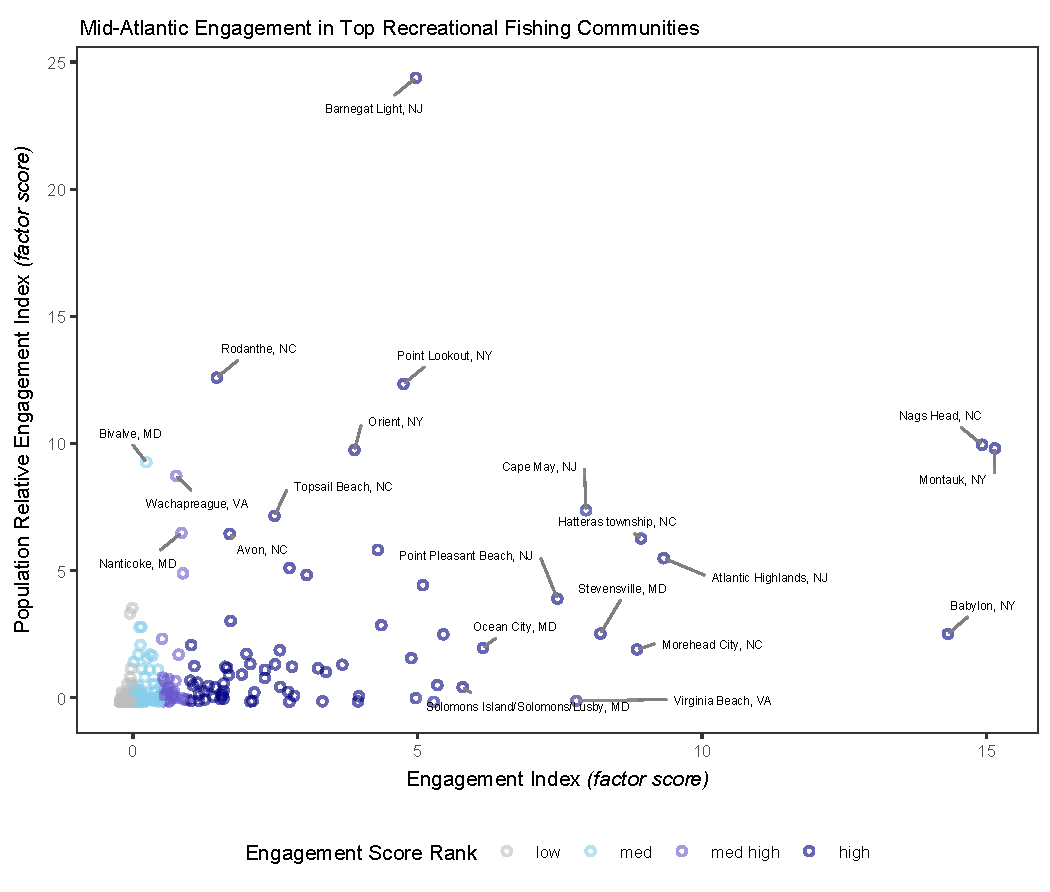
\includegraphics{midatlantic_files/figure-latex/recreational-engagement-1} 

}

\caption{Recreational engagement and population relative engagement with labels for the top recreationally engaged fishing communities in the Mid-Atlantic.}\label{fig:recreational-engagement}
\end{figure}

\global\setlength{\Oldarrayrulewidth}{\arrayrulewidth}

\global\setlength{\Oldtabcolsep}{\tabcolsep}

\setlength{\tabcolsep}{2pt}

\renewcommand*{\arraystretch}{1.5}



\providecommand{\ascline}[3]{\noalign{\global\arrayrulewidth #1}\arrayrulecolor[HTML]{#2}\cline{#3}}

\begin{longtable}[c]{|p{2.43in}|p{1.38in}|p{1.61in}|p{0.71in}}

\caption{Socio-demographic\ indicator\ rankings\ (ranging\ from\ low\ =\ low\ vulnerability\ to\ high\ =\ high\ vulnerability)\ for\ Mid-Atlantic\ communities\ most\ engaged\ in\ commercial\ fishing,\ 2022.\ Blank\ spaces\ indicate\ no\ data\ available.}\label{tab:recvultab}\\

\ascline{1.5pt}{666666}{1-4}

\multicolumn{1}{>{\raggedright}m{\dimexpr 2.43in+0\tabcolsep}}{\textcolor[HTML]{000000}{\fontsize{9}{9}\selectfont{Community}}} & \multicolumn{1}{>{\raggedright}m{\dimexpr 1.38in+0\tabcolsep}}{\textcolor[HTML]{000000}{\fontsize{9}{9}\selectfont{Personal\ Disruption}}} & \multicolumn{1}{>{\raggedright}m{\dimexpr 1.61in+0\tabcolsep}}{\textcolor[HTML]{000000}{\fontsize{9}{9}\selectfont{Population\ Composition}}} & \multicolumn{1}{>{\raggedright}m{\dimexpr 0.71in+0\tabcolsep}}{\textcolor[HTML]{000000}{\fontsize{9}{9}\selectfont{Poverty}}} \\

\ascline{1.5pt}{666666}{1-4}\endfirsthead \caption[]{Socio-demographic\ indicator\ rankings\ (ranging\ from\ low\ =\ low\ vulnerability\ to\ high\ =\ high\ vulnerability)\ for\ Mid-Atlantic\ communities\ most\ engaged\ in\ commercial\ fishing,\ 2022.\ Blank\ spaces\ indicate\ no\ data\ available.}\label{tab:recvultab}\\

\ascline{1.5pt}{666666}{1-4}

\multicolumn{1}{>{\raggedright}m{\dimexpr 2.43in+0\tabcolsep}}{\textcolor[HTML]{000000}{\fontsize{9}{9}\selectfont{Community}}} & \multicolumn{1}{>{\raggedright}m{\dimexpr 1.38in+0\tabcolsep}}{\textcolor[HTML]{000000}{\fontsize{9}{9}\selectfont{Personal\ Disruption}}} & \multicolumn{1}{>{\raggedright}m{\dimexpr 1.61in+0\tabcolsep}}{\textcolor[HTML]{000000}{\fontsize{9}{9}\selectfont{Population\ Composition}}} & \multicolumn{1}{>{\raggedright}m{\dimexpr 0.71in+0\tabcolsep}}{\textcolor[HTML]{000000}{\fontsize{9}{9}\selectfont{Poverty}}} \\

\ascline{1.5pt}{666666}{1-4}\endhead



\multicolumn{1}{>{\raggedright}m{\dimexpr 2.43in+0\tabcolsep}}{\textcolor[HTML]{000000}{\fontsize{9}{9}\selectfont{Cape\ May,\ NJ}}} & \multicolumn{1}{>{\raggedright}m{\dimexpr 1.38in+0\tabcolsep}}{\textcolor[HTML]{000000}{\fontsize{9}{9}\selectfont{low}}} & \multicolumn{1}{>{\raggedright}m{\dimexpr 1.61in+0\tabcolsep}}{\textcolor[HTML]{000000}{\fontsize{9}{9}\selectfont{med}}} & \multicolumn{1}{>{\raggedright}m{\dimexpr 0.71in+0\tabcolsep}}{\textcolor[HTML]{000000}{\fontsize{9}{9}\selectfont{low}}} \\





\multicolumn{1}{>{\raggedright}m{\dimexpr 2.43in+0\tabcolsep}}{\textcolor[HTML]{000000}{\fontsize{9}{9}\selectfont{Montauk,\ NY}}} & \multicolumn{1}{>{\raggedright}m{\dimexpr 1.38in+0\tabcolsep}}{\textcolor[HTML]{000000}{\fontsize{9}{9}\selectfont{low}}} & \multicolumn{1}{>{\raggedright}m{\dimexpr 1.61in+0\tabcolsep}}{\textcolor[HTML]{000000}{\fontsize{9}{9}\selectfont{low}}} & \multicolumn{1}{>{\raggedright}m{\dimexpr 0.71in+0\tabcolsep}}{\textcolor[HTML]{000000}{\fontsize{9}{9}\selectfont{low}}} \\





\multicolumn{1}{>{\raggedright}m{\dimexpr 2.43in+0\tabcolsep}}{\textcolor[HTML]{000000}{\fontsize{9}{9}\selectfont{Point\ Pleasant\ Beach,\ NJ}}} & \multicolumn{1}{>{\raggedright}m{\dimexpr 1.38in+0\tabcolsep}}{\textcolor[HTML]{000000}{\fontsize{9}{9}\selectfont{med}}} & \multicolumn{1}{>{\raggedright}m{\dimexpr 1.61in+0\tabcolsep}}{\textcolor[HTML]{000000}{\fontsize{9}{9}\selectfont{low}}} & \multicolumn{1}{>{\raggedright}m{\dimexpr 0.71in+0\tabcolsep}}{\textcolor[HTML]{000000}{\fontsize{9}{9}\selectfont{low}}} \\





\multicolumn{1}{>{\raggedright}m{\dimexpr 2.43in+0\tabcolsep}}{\textcolor[HTML]{000000}{\fontsize{9}{9}\selectfont{Barnegat\ Light,\ NJ}}} & \multicolumn{1}{>{\raggedright}m{\dimexpr 1.38in+0\tabcolsep}}{\textcolor[HTML]{000000}{\fontsize{9}{9}\selectfont{low}}} & \multicolumn{1}{>{\raggedright}m{\dimexpr 1.61in+0\tabcolsep}}{\textcolor[HTML]{000000}{\fontsize{9}{9}\selectfont{low}}} & \multicolumn{1}{>{\raggedright}m{\dimexpr 0.71in+0\tabcolsep}}{\textcolor[HTML]{000000}{\fontsize{9}{9}\selectfont{low}}} \\





\multicolumn{1}{>{\raggedright}m{\dimexpr 2.43in+0\tabcolsep}}{\textcolor[HTML]{000000}{\fontsize{9}{9}\selectfont{Ocean\ City,\ MD}}} & \multicolumn{1}{>{\raggedright}m{\dimexpr 1.38in+0\tabcolsep}}{\textcolor[HTML]{000000}{\fontsize{9}{9}\selectfont{med}}} & \multicolumn{1}{>{\raggedright}m{\dimexpr 1.61in+0\tabcolsep}}{\textcolor[HTML]{000000}{\fontsize{9}{9}\selectfont{low}}} & \multicolumn{1}{>{\raggedright}m{\dimexpr 0.71in+0\tabcolsep}}{\textcolor[HTML]{000000}{\fontsize{9}{9}\selectfont{low}}} \\





\multicolumn{1}{>{\raggedright}m{\dimexpr 2.43in+0\tabcolsep}}{\textcolor[HTML]{000000}{\fontsize{9}{9}\selectfont{Virginia\ Beach,\ VA}}} & \multicolumn{1}{>{\raggedright}m{\dimexpr 1.38in+0\tabcolsep}}{\textcolor[HTML]{000000}{\fontsize{9}{9}\selectfont{low}}} & \multicolumn{1}{>{\raggedright}m{\dimexpr 1.61in+0\tabcolsep}}{\textcolor[HTML]{000000}{\fontsize{9}{9}\selectfont{low}}} & \multicolumn{1}{>{\raggedright}m{\dimexpr 0.71in+0\tabcolsep}}{\textcolor[HTML]{000000}{\fontsize{9}{9}\selectfont{low}}} \\





\multicolumn{1}{>{\raggedright}m{\dimexpr 2.43in+0\tabcolsep}}{\textcolor[HTML]{000000}{\fontsize{9}{9}\selectfont{Morehead\ City,\ NC}}} & \multicolumn{1}{>{\raggedright}m{\dimexpr 1.38in+0\tabcolsep}}{\textcolor[HTML]{000000}{\fontsize{9}{9}\selectfont{med}}} & \multicolumn{1}{>{\raggedright}m{\dimexpr 1.61in+0\tabcolsep}}{\textcolor[HTML]{000000}{\fontsize{9}{9}\selectfont{low}}} & \multicolumn{1}{>{\raggedright}m{\dimexpr 0.71in+0\tabcolsep}}{\textcolor[HTML]{000000}{\fontsize{9}{9}\selectfont{med}}} \\





\multicolumn{1}{>{\raggedright}m{\dimexpr 2.43in+0\tabcolsep}}{\textcolor[HTML]{000000}{\fontsize{9}{9}\selectfont{Hatteras\ township,\ NC}}} & \multicolumn{1}{>{\raggedright}m{\dimexpr 1.38in+0\tabcolsep}}{\textcolor[HTML]{000000}{\fontsize{9}{9}\selectfont{low}}} & \multicolumn{1}{>{\raggedright}m{\dimexpr 1.61in+0\tabcolsep}}{\textcolor[HTML]{000000}{\fontsize{9}{9}\selectfont{low}}} & \multicolumn{1}{>{\raggedright}m{\dimexpr 0.71in+0\tabcolsep}}{\textcolor[HTML]{000000}{\fontsize{9}{9}\selectfont{low}}} \\





\multicolumn{1}{>{\raggedright}m{\dimexpr 2.43in+0\tabcolsep}}{\textcolor[HTML]{000000}{\fontsize{9}{9}\selectfont{Wachapreague,\ VA}}} & \multicolumn{1}{>{\raggedright}m{\dimexpr 1.38in+0\tabcolsep}}{\textcolor[HTML]{000000}{\fontsize{9}{9}\selectfont{low}}} & \multicolumn{1}{>{\raggedright}m{\dimexpr 1.61in+0\tabcolsep}}{\textcolor[HTML]{000000}{\fontsize{9}{9}\selectfont{low}}} & \multicolumn{1}{>{\raggedright}m{\dimexpr 0.71in+0\tabcolsep}}{\textcolor[HTML]{000000}{\fontsize{9}{9}\selectfont{low}}} \\





\multicolumn{1}{>{\raggedright}m{\dimexpr 2.43in+0\tabcolsep}}{\textcolor[HTML]{000000}{\fontsize{9}{9}\selectfont{Avon,\ NC}}} & \multicolumn{1}{>{\raggedright}m{\dimexpr 1.38in+0\tabcolsep}}{\textcolor[HTML]{000000}{\fontsize{9}{9}\selectfont{high}}} & \multicolumn{1}{>{\raggedright}m{\dimexpr 1.61in+0\tabcolsep}}{\textcolor[HTML]{000000}{\fontsize{9}{9}\selectfont{low}}} & \multicolumn{1}{>{\raggedright}m{\dimexpr 0.71in+0\tabcolsep}}{\textcolor[HTML]{000000}{\fontsize{9}{9}\selectfont{}}} \\





\multicolumn{1}{>{\raggedright}m{\dimexpr 2.43in+0\tabcolsep}}{\textcolor[HTML]{000000}{\fontsize{9}{9}\selectfont{Atlantic\ Highlands,\ NJ}}} & \multicolumn{1}{>{\raggedright}m{\dimexpr 1.38in+0\tabcolsep}}{\textcolor[HTML]{000000}{\fontsize{9}{9}\selectfont{low}}} & \multicolumn{1}{>{\raggedright}m{\dimexpr 1.61in+0\tabcolsep}}{\textcolor[HTML]{000000}{\fontsize{9}{9}\selectfont{low}}} & \multicolumn{1}{>{\raggedright}m{\dimexpr 0.71in+0\tabcolsep}}{\textcolor[HTML]{000000}{\fontsize{9}{9}\selectfont{low}}} \\





\multicolumn{1}{>{\raggedright}m{\dimexpr 2.43in+0\tabcolsep}}{\textcolor[HTML]{000000}{\fontsize{9}{9}\selectfont{Babylon,\ NY}}} & \multicolumn{1}{>{\raggedright}m{\dimexpr 1.38in+0\tabcolsep}}{\textcolor[HTML]{000000}{\fontsize{9}{9}\selectfont{low}}} & \multicolumn{1}{>{\raggedright}m{\dimexpr 1.61in+0\tabcolsep}}{\textcolor[HTML]{000000}{\fontsize{9}{9}\selectfont{low}}} & \multicolumn{1}{>{\raggedright}m{\dimexpr 0.71in+0\tabcolsep}}{\textcolor[HTML]{000000}{\fontsize{9}{9}\selectfont{low}}} \\





\multicolumn{1}{>{\raggedright}m{\dimexpr 2.43in+0\tabcolsep}}{\textcolor[HTML]{000000}{\fontsize{9}{9}\selectfont{Nags\ Head,\ NC}}} & \multicolumn{1}{>{\raggedright}m{\dimexpr 1.38in+0\tabcolsep}}{\textcolor[HTML]{000000}{\fontsize{9}{9}\selectfont{low}}} & \multicolumn{1}{>{\raggedright}m{\dimexpr 1.61in+0\tabcolsep}}{\textcolor[HTML]{000000}{\fontsize{9}{9}\selectfont{low}}} & \multicolumn{1}{>{\raggedright}m{\dimexpr 0.71in+0\tabcolsep}}{\textcolor[HTML]{000000}{\fontsize{9}{9}\selectfont{low}}} \\





\multicolumn{1}{>{\raggedright}m{\dimexpr 2.43in+0\tabcolsep}}{\textcolor[HTML]{000000}{\fontsize{9}{9}\selectfont{Point\ Lookout,\ NY}}} & \multicolumn{1}{>{\raggedright}m{\dimexpr 1.38in+0\tabcolsep}}{\textcolor[HTML]{000000}{\fontsize{9}{9}\selectfont{low}}} & \multicolumn{1}{>{\raggedright}m{\dimexpr 1.61in+0\tabcolsep}}{\textcolor[HTML]{000000}{\fontsize{9}{9}\selectfont{low}}} & \multicolumn{1}{>{\raggedright}m{\dimexpr 0.71in+0\tabcolsep}}{\textcolor[HTML]{000000}{\fontsize{9}{9}\selectfont{low}}} \\





\multicolumn{1}{>{\raggedright}m{\dimexpr 2.43in+0\tabcolsep}}{\textcolor[HTML]{000000}{\fontsize{9}{9}\selectfont{Nanticoke,\ MD}}} & \multicolumn{1}{>{\raggedright}m{\dimexpr 1.38in+0\tabcolsep}}{\textcolor[HTML]{000000}{\fontsize{9}{9}\selectfont{med\ high}}} & \multicolumn{1}{>{\raggedright}m{\dimexpr 1.61in+0\tabcolsep}}{\textcolor[HTML]{000000}{\fontsize{9}{9}\selectfont{low}}} & \multicolumn{1}{>{\raggedright}m{\dimexpr 0.71in+0\tabcolsep}}{\textcolor[HTML]{000000}{\fontsize{9}{9}\selectfont{low}}} \\





\multicolumn{1}{>{\raggedright}m{\dimexpr 2.43in+0\tabcolsep}}{\textcolor[HTML]{000000}{\fontsize{9}{9}\selectfont{Orient,\ NY}}} & \multicolumn{1}{>{\raggedright}m{\dimexpr 1.38in+0\tabcolsep}}{\textcolor[HTML]{000000}{\fontsize{9}{9}\selectfont{low}}} & \multicolumn{1}{>{\raggedright}m{\dimexpr 1.61in+0\tabcolsep}}{\textcolor[HTML]{000000}{\fontsize{9}{9}\selectfont{low}}} & \multicolumn{1}{>{\raggedright}m{\dimexpr 0.71in+0\tabcolsep}}{\textcolor[HTML]{000000}{\fontsize{9}{9}\selectfont{}}} \\





\multicolumn{1}{>{\raggedright}m{\dimexpr 2.43in+0\tabcolsep}}{\textcolor[HTML]{000000}{\fontsize{9}{9}\selectfont{Bivalve,\ MD}}} & \multicolumn{1}{>{\raggedright}m{\dimexpr 1.38in+0\tabcolsep}}{\textcolor[HTML]{000000}{\fontsize{9}{9}\selectfont{med}}} & \multicolumn{1}{>{\raggedright}m{\dimexpr 1.61in+0\tabcolsep}}{\textcolor[HTML]{000000}{\fontsize{9}{9}\selectfont{high}}} & \multicolumn{1}{>{\raggedright}m{\dimexpr 0.71in+0\tabcolsep}}{\textcolor[HTML]{000000}{\fontsize{9}{9}\selectfont{}}} \\





\multicolumn{1}{>{\raggedright}m{\dimexpr 2.43in+0\tabcolsep}}{\textcolor[HTML]{000000}{\fontsize{9}{9}\selectfont{Rodanthe,\ NC}}} & \multicolumn{1}{>{\raggedright}m{\dimexpr 1.38in+0\tabcolsep}}{\textcolor[HTML]{000000}{\fontsize{9}{9}\selectfont{low}}} & \multicolumn{1}{>{\raggedright}m{\dimexpr 1.61in+0\tabcolsep}}{\textcolor[HTML]{000000}{\fontsize{9}{9}\selectfont{low}}} & \multicolumn{1}{>{\raggedright}m{\dimexpr 0.71in+0\tabcolsep}}{\textcolor[HTML]{000000}{\fontsize{9}{9}\selectfont{}}} \\





\multicolumn{1}{>{\raggedright}m{\dimexpr 2.43in+0\tabcolsep}}{\textcolor[HTML]{000000}{\fontsize{9}{9}\selectfont{Topsail\ Beach,\ NC}}} & \multicolumn{1}{>{\raggedright}m{\dimexpr 1.38in+0\tabcolsep}}{\textcolor[HTML]{000000}{\fontsize{9}{9}\selectfont{low}}} & \multicolumn{1}{>{\raggedright}m{\dimexpr 1.61in+0\tabcolsep}}{\textcolor[HTML]{000000}{\fontsize{9}{9}\selectfont{low}}} & \multicolumn{1}{>{\raggedright}m{\dimexpr 0.71in+0\tabcolsep}}{\textcolor[HTML]{000000}{\fontsize{9}{9}\selectfont{low}}} \\





\multicolumn{1}{>{\raggedright}m{\dimexpr 2.43in+0\tabcolsep}}{\textcolor[HTML]{000000}{\fontsize{9}{9}\selectfont{Solomons\ Island/Solomons/Lusby,\ MD}}} & \multicolumn{1}{>{\raggedright}m{\dimexpr 1.38in+0\tabcolsep}}{\textcolor[HTML]{000000}{\fontsize{9}{9}\selectfont{low}}} & \multicolumn{1}{>{\raggedright}m{\dimexpr 1.61in+0\tabcolsep}}{\textcolor[HTML]{000000}{\fontsize{9}{9}\selectfont{low}}} & \multicolumn{1}{>{\raggedright}m{\dimexpr 0.71in+0\tabcolsep}}{\textcolor[HTML]{000000}{\fontsize{9}{9}\selectfont{low}}} \\





\multicolumn{1}{>{\raggedright}m{\dimexpr 2.43in+0\tabcolsep}}{\textcolor[HTML]{000000}{\fontsize{9}{9}\selectfont{Stevensville,\ MD}}} & \multicolumn{1}{>{\raggedright}m{\dimexpr 1.38in+0\tabcolsep}}{\textcolor[HTML]{000000}{\fontsize{9}{9}\selectfont{med}}} & \multicolumn{1}{>{\raggedright}m{\dimexpr 1.61in+0\tabcolsep}}{\textcolor[HTML]{000000}{\fontsize{9}{9}\selectfont{low}}} & \multicolumn{1}{>{\raggedright}m{\dimexpr 0.71in+0\tabcolsep}}{\textcolor[HTML]{000000}{\fontsize{9}{9}\selectfont{low}}} \\

\ascline{1.5pt}{666666}{1-4}



\end{longtable}



\arrayrulecolor[HTML]{000000}

\global\setlength{\arrayrulewidth}{\Oldarrayrulewidth}

\global\setlength{\tabcolsep}{\Oldtabcolsep}

\renewcommand*{\arraystretch}{1}

\subsubsection{Indicators: Community Climate Vulnerability in the Mid-Atlantic}\label{indicators-community-climate-vulnerability-in-the-mid-atlantic}

The \href{https://noaa-edab.github.io/catalog/community_climate_vulnerability.html}{Community Climate Change Risk Indicators} are calculated by multiplying the percent contribution of species to the total value landed in a community by their respective Total Vulnerability scores (based on NOAA's Climate Vulnerability Assessment) for different sensitivity and exposure factors and then summing the resulting values by year. As a community (or region) shifts towards climate vulnerable species, its risk score increases. While there is not a long-term trend in total climate vulnerability across Mid Atlantic communities as a whole, a majority of communities rank either high or very high risk (Fig. \ref{fig:commvulex}). This suggests that a majority of Mid-Atlantic communities depend on climate vulnerable species to generate commercial fishery revenue.

\begin{figure}

{\centering 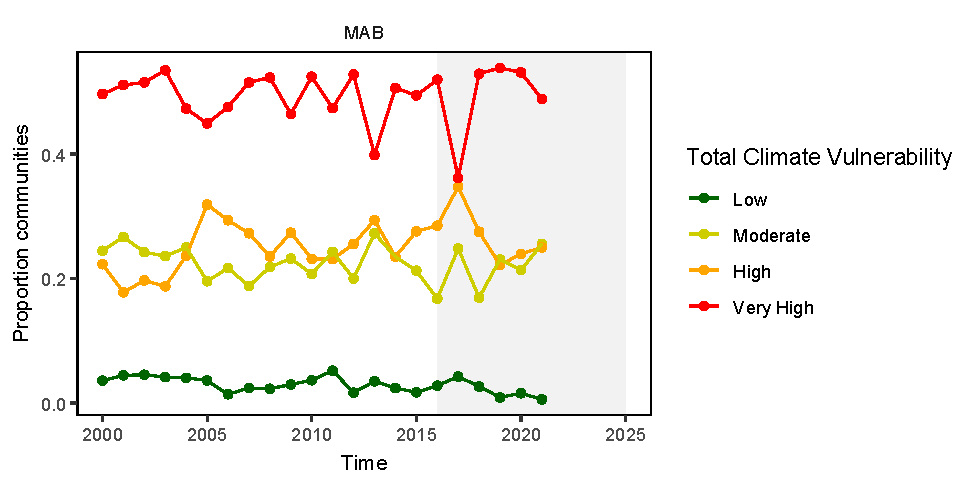
\includegraphics{midatlantic_files/figure-latex/commvulex-1} 

}

\caption{Proportion of Mid-Atlantic communities at each revenue climate vulnerability level over time.}\label{fig:commvulex}
\end{figure}

\subsubsection{Implications}\label{implications-4}

A range of socioeconomic and climate vulnerability concerns are found throughout Mid-Atlantic fishing communities. These indicators provide a snapshot of the presence of socio-demographic concerns in most highly engaged commercial and recreational fishing communities in the Mid-Atlantic. These communities may be especially vulnerable to changes in fishing patterns due to regulations and/or ecosystem changes. Several of these top fishing communities, both commercial and recreational fishing communities, demonstrated medium to high socio-demographic vulnerability, indicating that they may be at a disadvantage responding to change.

There is evidence that a majority of Mid-Atlantic communities have high to very high total climate vulnerability based on revenue. Coastal fishing communities are greatly affected by climate change, both because of their physical location and because of their frequent social, cultural, and economic dependence on fishing. These impacts are expected to become more pressing as climatic changes become more extensive. Changes in \href{https://noaa-edab.github.io/catalog/bottom_temp_insitu.html}{ocean temperature} and \href{https://noaa-edab.github.io/catalog/ocean_acidification.html}{acidification} affecting marine life have the potential to directly impact fisheries and fishery dependent livelihoods.

\begin{verbatim}
## [1] "Ending 05_csvi_midatlantic.Rmd"
\end{verbatim}

\subsection{Protected Species}\label{protected-species}

Fishery management objectives for protected species generally focus on reducing threats and on habitat conservation/restoration. Protected species include marine mammals protected under the Marine Mammal Protection Act, endangered and threatened species protected under the Endangered Species Act, and migratory birds protected under the Migratory Bird Treaty Act. In the Northeast U.S., endangered/threatened species include Atlantic salmon, Atlantic and shortnose sturgeon, all sea turtle species, giant manta ray, oceanic whitetip shark, and five baleen whales. Protected species objectives include managing bycatch to remain below potential biological removal (PBR) thresholds, recovering endangered populations, and monitoring unusual mortality events (UMEs). Here we report on performance relative to these objectives with available indicator data, as well as indicating the potential for future interactions driven by observed and predicted ecosystem changes in the Northeast U.S.

\subsubsection{Indicators: bycatch, population (adult and juvenile) numbers, mortalities}\label{indicators-bycatch-population-adult-and-juvenile-numbers-mortalities}

Average indices for both \href{https://noaa-edab.github.io/catalog/harborporpoise.html}{harbor porpoise} (Fig. \ref{fig:harborporpoise}) and \href{https://noaa-edab.github.io/catalog/grayseal.html}{gray seal} bycatch (Fig. \ref{fig:grayseal}) are below current PBR thresholds, meeting management objectives, although uncertainty in the gray seal bycatch estimate has increased recently, and gray seal bycatch is among the highest for marine mammals in the U.S.

\begin{figure}

{\centering 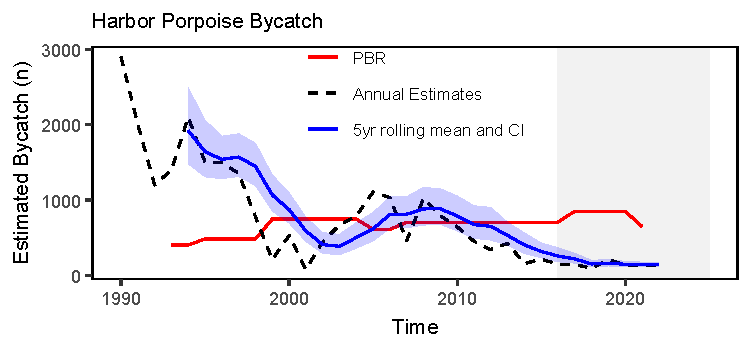
\includegraphics{midatlantic_files/figure-latex/harborporpoise-1} 

}

\caption{Harbor porpoise average bycatch estimate for Mid-Atlantic and New England gillnet fisheries (blue) and the potential biological removal (red).}\label{fig:harborporpoise}
\end{figure}

The annual estimate for gray seal bycatch, most of which occurs in New England, has declined since 2019, in part driven by declining gillnet landings. In addition, estimates since 2019 have greater uncertainty stemming from low observer coverage in some times and areas since 2019. The rolling mean confidence interval remains just below the PBR threshold.

\begin{figure}

{\centering 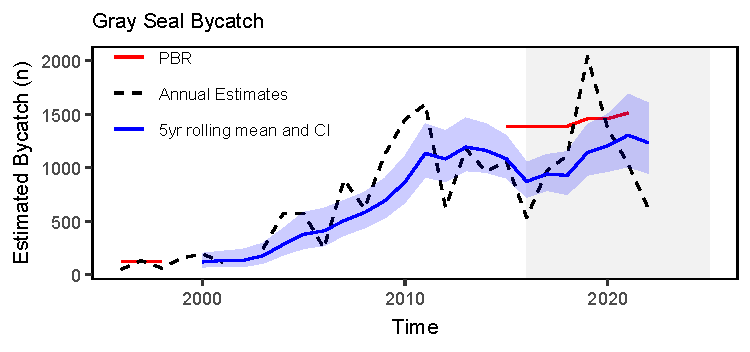
\includegraphics{midatlantic_files/figure-latex/grayseal-1} 

}

\caption{Gray Seal average bycatch estimate for gillnet fisheries (blue) and the potential biological removal (red).}\label{fig:grayseal}
\end{figure}

The \href{https://noaa-edab.github.io/catalog/narw.html}{North Atlantic right whale population} was on a recovery trajectory until 2010, but has since declined (Fig. \ref{fig:narw-abundance}). The sharp decline observed from 2015-2020 appears to have slowed, although the right whale population continues to experience annual mortalities above recovery thresholds. Reduced survival rates of adult females lead to diverging abundance trends between sexes. It is estimated that there are fewer than 70 adult females remaining in the population.

\begin{figure}

{\centering 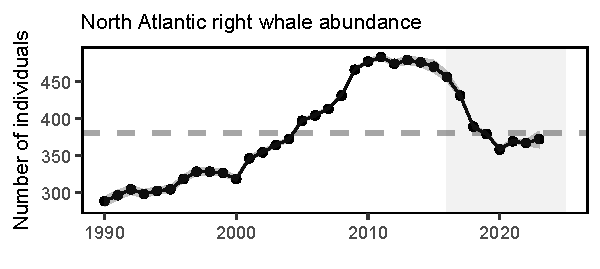
\includegraphics{midatlantic_files/figure-latex/narw-abundance-1} 

}

\caption{Estimated North Atlanic right whale abundance on the Northeast Shelf.}\label{fig:narw-abundance}
\end{figure}

North Atlantic right whale \href{https://noaa-edab.github.io/catalog/narw.html}{calf counts} have generally declined after 2009 to the point of having zero new calves observed in 2018 (Fig. \ref{fig:NARW-calf-abundance}). However, since 2020, calf births have been closer to the long-term average.

\begin{figure}

{\centering 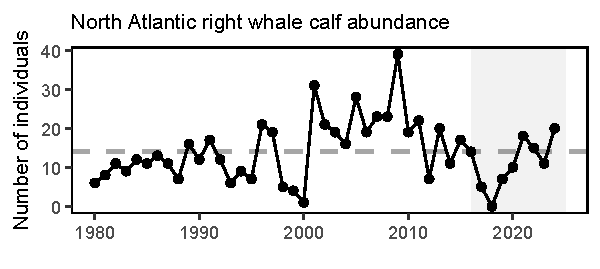
\includegraphics{midatlantic_files/figure-latex/NARW-calf-abundance-1} 

}

\caption{Number of North Atlantic right whale calf births, 1990 - 2022.}\label{fig:NARW-calf-abundance}
\end{figure}

This year, the Unusual Mortality Event (UME) for North Atlantic right whales continued. From 2017 through 2 January 2025, the total UME right whale mortalities includes 41 dead stranded whales, 19 in the US and 22 in Canada. When alive but seriously injured whales (39) and sublethal injuries or ill whales (71) are taken into account, 151 individual whales are included in the UME. Recent research suggests that many mortalities go unobserved and the true number of mortalities are about three times the count of the observed mortalities. The primary cause of death is ``human interaction'' from entanglements or vessel strikes.

A UME continued from previous years for humpback whales (2016-present) and Atlantic minke whales (2018-present); suspected causes include human interactions. A UME for Northeast pinnipeds that began in 2018 for infectious disease is pending closure as of February 2025.

\subsubsection{Implications}\label{implications-5}

Bycatch management measures have been implemented to maintain bycatch below PBR thresholds. The downward trend in harbor porpoise bycatch could also be due to a decrease in harbor porpoise abundance in U.S. waters, reducing their overlap with fisheries, and a decrease in gillnet effort. The increasing trend in gray seal bycatch may be related to an increase in the gray seal population (\href{https://noaa-edab.github.io/catalog/seal_pups.html}{U.S. pup counts}), supported by the dramatic rise over the last three decades in observed numbers of gray seal pups born at U.S. breeding sites plus an increase in adult seals at the breeding sites, some of which are supplemented by Canadian adults.

Strong evidence exists to suggest that interactions between right whales and both the fixed gear fisheries in the U.S. and Canada and vessel strikes in the U.S. are contributing substantially to the decline of the species. Further, right whale distribution has changed since 2010. \href{https://noaa-edab.github.io/catalog/narw.html}{Recent research} suggests that recent climate driven changes in ocean circulation have resulted in right whale distribution changes driven by increased warm water influx through the Northeast Channel, which has reduced the primary right whale prey (the copepod \emph{Calanus finmarchicus}) in the central and eastern portions of the Gulf of Maine. Additional potential stressors include offshore wind development, which overlaps with important habitat areas used year-round by right whales, including mother and calf migration corridors and foraging habitat. This area is also a primary right whale winter foraging habitat. Additional information can be found in the \hyperref[other-ocean-uses-offshore-wind]{offshore wind risks section}.

The UMEs are under investigation and are likely the result of multiple drivers. For all large whale UMEs, human interaction appears to have contributed to increased mortalities, although investigations are not complete.

A climate vulnerability assessment is published for Atlantic and Gulf marine mammal populations.

\section{Risks to Meeting Fishery Management Objectives}\label{risks-to-meeting-fishery-management-objectives}

\subsection{Climate and Ecosystem Change}\label{climate-and-ecosystem-change}

\subsubsection{Risks to managing spatially}\label{risks-to-managing-spatially}

Shifting species distributions (changes in spatial extent or center of gravity) alter both species interactions and fishery interactions. In particular, shifting species distributions can affect expected management outcomes from spatial allocations and bycatch measures based on historical fish and protected species distributions. Species availability to surveys can also change as distributions shift within survey footprints, complicating the interpretation of survey trends.

Coastwide indicators are reviewed in this section to evaluate spatial change throughout the Northeast US shelf. Indicators are identical between the Mid Atlantic and New England reports.

\paragraph{Indicators: Fish and protected species distribution shifts}\label{indicators-fish-and-protected-species-distribution-shifts}

As noted in the \hyperref[implications]{Seafood Production Implications section above}, the center of \href{https://noaa-edab.github.io/catalog/species_dist.html}{distribution} for a suite of 48 commercially or ecologically important fish species combined along the entire Northeast Shelf continues to show movement towards the northeast and generally into deeper water (Fig. \ref{fig:species-dist}). Distribution shifts have been noted for several \href{https://noaa-edab.github.io/catalog/species_dist.html}{highly migratory species}, including sharks, billfish and tunas between 2002 and 2019.

\href{https://noaa-edab.github.io/catalog/habitat_diversity.html}{Habitat model-based species richness} suggests shifts of both cooler and warmer water species to the northeast. Similar patterns have been found for \href{https://noaa-edab.github.io/catalog/cetacean_dist.html}{marine mammals}, with multiple species shifting northeast between 2010 and 2017 in most seasons (Fig. \ref{fig:protectedspp-dist-shifts}).

\begin{figure}

{\centering 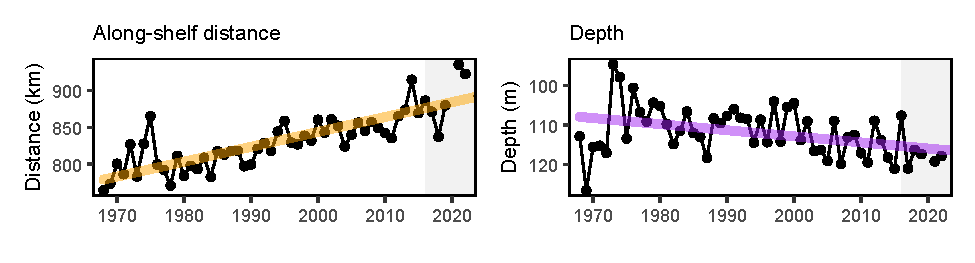
\includegraphics{midatlantic_files/figure-latex/species-dist-1} 

}

\caption{Aggregate species distribution metrics for species in the Northeast Large Marine Ecosystem: along shelf distance with increasing trend (orange), and depth with decreasing trend indicating deeper water (purple).}\label{fig:species-dist}
\end{figure}

\begin{figure}

{\centering 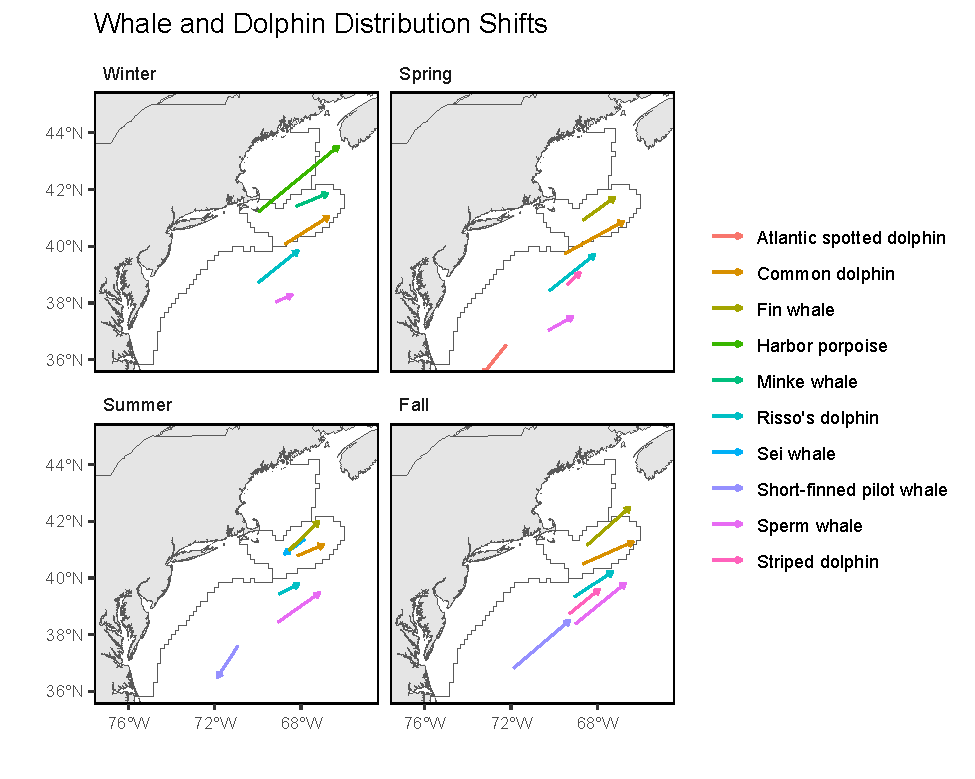
\includegraphics{midatlantic_files/figure-latex/protectedspp-dist-shifts-1} 

}

\caption{Direction and magnitude of core habitat shifts, represented by the length of the line of the seasonal weighted centroid for species with more than 70 km difference between 2010 and 2017 (tip of arrow).}\label{fig:protectedspp-dist-shifts}
\end{figure}

\paragraph{Drivers:}\label{drivers}

Mobile populations shift distributions to maintain suitable temperature and prey fields, possibly expanding ranges if new suitable habitat exists. Changes in managed species distribution is related, in part, to the \href{https://noaa-edab.github.io/catalog/forage_index.html}{distribution of forage biomass}. Since 1982, the fall center of gravity of forage fish (20 species combined) has moved to the north and east (Fig. \ref{fig:forageshifts}). Spring forage fish center of gravity has been more variable over time. \href{https://noaa-edab.github.io/catalog/zooplankton_index.html\#key-results-and-visualizations-4}{Small copepods}, widespread prey of many larval and juvenile fish, show a similar shift in center of gravity as forage fish, to the north and east in the fall, as well as northward in spring.

\begin{figure}

{\centering 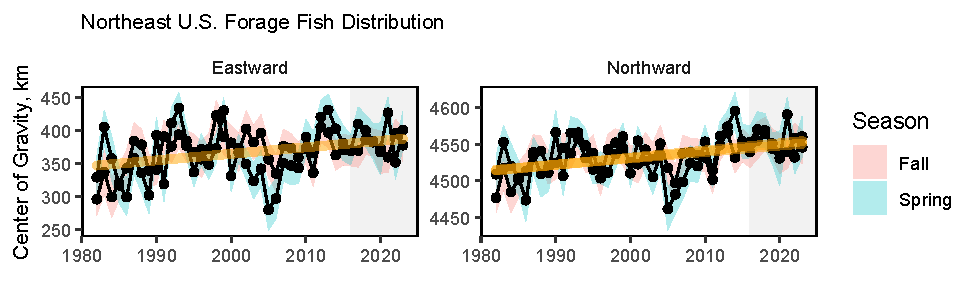
\includegraphics{midatlantic_files/figure-latex/forageshifts-1} 

}

\caption{Eastward (left) and northward (right) shifts in the center of gravity for 20 forage fish species on the Northeast U.S. Shelf, with increasing trend (orange) for fall eastward and northward center of gravity.}\label{fig:forageshifts}
\end{figure}

In contrast, \href{https://noaa-edab.github.io/catalog/benthos_index.html}{macrobenthos} center of gravity has shifted westward (Fig. \ref{fig:macrobenthosshifts}). Macrobenthos are small bottom-dwelling invertebrates including polychaete worms, small crustaceans, bivalves (non-commercial), gastropods, nemerteans, tunicates, cnidarians, brittle stars, sea cucumbers, and sand dollars, and are prey for many managed species. \href{https://noaa-edab.github.io/catalog/zooplankton_index.html\#key-results-and-visualizations-4}{Large copepods} have a similar pattern to macrobenthos, trending westward in fall.

\begin{figure}

{\centering 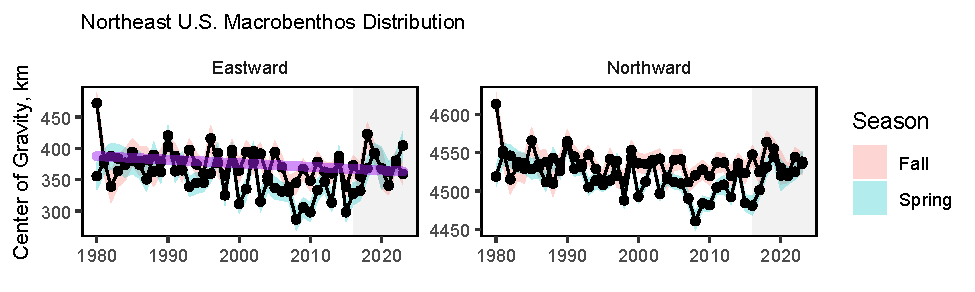
\includegraphics{midatlantic_files/figure-latex/macrobenthosshifts-1} 

}

\caption{Eastward (left) and northward (right) shifts in the center of gravity for macrobenthos species on the Northeast U.S. Shelf}\label{fig:macrobenthosshifts}
\end{figure}

Ocean temperatures influence the distribution, seasonal timing, and productivity of managed species (see sections below). The Northeast US shelf, including the Mid-Atlantic, has experienced a continued warming trend for both the \href{https://noaa-edab.github.io/catalog/long_term_sst.html}{long term annual sea surface} (Fig. \ref{fig:long-term-sst}) and \href{https://noaa-edab.github.io/catalog/seasonal_oisst_anom.html}{seasonal surface} and \href{https://noaa-edab.github.io/catalog/bottom_temp_model_anom.html}{bottom temperature}. However, 2024 surface and bottom temperatures were near normal to cooler than normal conditions in all seasons in the MAB (see also the \hyperref[highlights]{2024 Highlights section}).

\begin{figure}

{\centering 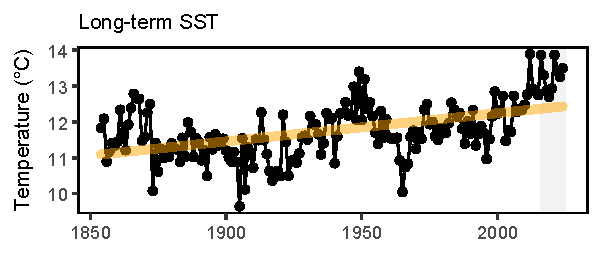
\includegraphics{midatlantic_files/figure-latex/long-term-sst-1} 

}

\caption{Northeast US annual sea surface temperature (SST, black), with increasing trend (orange).}\label{fig:long-term-sst}
\end{figure}

Species suitable habitat can expand or contract when changes in temperature and major oceanographic conditions alter distinct water mass habitats.The variability of the Gulf Stream is a major driver of the predominant oceanographic conditions of the Northeast U.S. continental shelf. As the \href{https://noaa-edab.github.io/catalog/gsi.html}{Gulf Stream} has become less stable and shifted northward in the last decade (Fig. \ref{fig:GSI}), warmer ocean temperatures have been observed on the northeast shelf and a higher proportion of \href{https://noaa-edab.github.io/catalog/slopewater.html}{Warm Slope Water} has been present in the Northeast Channel. Since 2008, the Gulf Stream has moved closer to the Grand Banks, reducing the supply of cold, fresh, and oxygen-rich Labrador Current waters to the Northwest Atlantic Shelf. In 2024, however, the \href{https://noaa-edab.github.io/catalog/gsi.html}{eastern portion of the Gulf Stream was further south}, which could affect the composition of the source water entering the Gulf of Maine through the Northeast Channel (see \hyperref[highlights]{2024 Highlights}).

\begin{figure}

{\centering 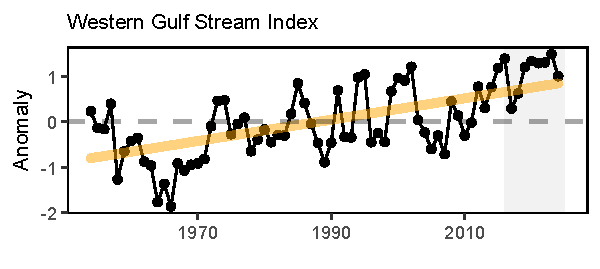
\includegraphics{midatlantic_files/figure-latex/GSI-1} 

}

\caption{Index representing changes in the location of the western (between 64 and 55 degrees W) Gulf Stream north wall (black). Positive values represent a more northerly Gulf Stream position, with increasing trend (orange).}\label{fig:GSI}
\end{figure}

Changes in ocean temperature and circulation alter habitat features such as the Middle Atlantic Bight \href{https://noaa-edab.github.io/catalog/cold_pool.html}{Cold Pool}, a band of relatively cold near-bottom water from spring to fall over the northern MAB. The cold pool represents essential fish spawning and nursery habitat, and affects fish distribution and behavior. The cold pool has been getting warmer and its areal extent has been shrinking over time (Fig. \ref{fig:cold-pool-size}). In 2024, however, the cold pool index and extent were near the long-term average, likely due to the influx of Labrador Slope and Scotian Shelf waters into the system.

\begin{figure}

{\centering 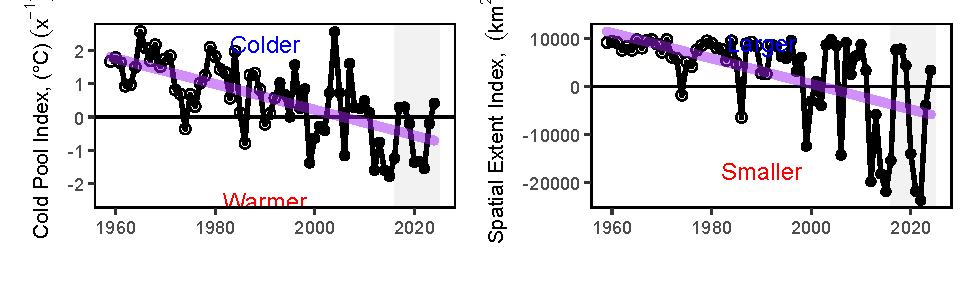
\includegraphics{midatlantic_files/figure-latex/cold-pool-size-1} 

}

\caption{Seasonal cold pool mean temperature (left) and spatial extent index (right), based on bias-corrected ROMS-NWA (open circles) and GLORYS (closed circles), with declining trends (purple).}\label{fig:cold-pool-size}
\end{figure}

\paragraph{Future Considerations}\label{future-considerations}

Distribution shifts caused by changes in thermal habitat and ocean circulation are likely to continue as long as long-term trends persist. Episodic and short-term events (see \hyperref[highlights]{2024 Highlights}) may increase variability in the trends, however species distributions are unlikely to reverse to historical ranges in the short term. Increased mechanistic understanding of distribution drivers is needed to better understand future distribution shifts: species with high mobility or short lifespans react differently from immobile or long lived species.

Long-term oceanographic projections forecast a temporary pause in warming over the next decade due to internal variability in circulation and a southward shift of the Gulf Stream. Near-term forecasts are being evaluated to determine how well they are able to predict episodic and anomalous events that are outside of the long-term patterns.

Adapting management to changing stock distributions and dynamic ocean processes will require continued monitoring of populations in space and evaluating management measures against a range of possible future spatial distributions. Processes like the \href{https://www.mafmc.org/climate-change-scenario-planning}{East Coast Climate Scenario Planning}, and subsequent formation of the \href{https://www.mafmc.org/e3cg}{East Coast Climate Coordination Group}, can help coordinate management.

\subsubsection{Risks to managing seasonally}\label{risks-to-managing-seasonally}

The effectiveness of seasonal management actions (fishing seasons or area opening/closing) depends on a proper alignment with the seasonal life cycle events (phenology) of fish stocks (e.g.~migration timing and spawning). Changes in the timing of these biological cycles can reduce the effectiveness of management measures if not accounted for. The timing of seasonal patterns can also change the interactions between fisheries and non-target species thus influencing the amount of bycatch and the availability of species to surveys.

\paragraph{Indicators: Timing shifts}\label{indicators-timing-shifts}

\href{https://noaa-edab.github.io/catalog/spawn_timing.html}{Spawning timing} is shifting earlier for multiple stocks, including haddock and yellowtail flounder. Spawning of both haddock stocks occurred earlier in the year, as indicated by more resting (post-spawning) stage fish in the 2010s as compared to earlier in the time series (Fig. \ref{fig:spawntiming}). The northern (Cape Cod/GOM) yellowtail flounder stock shows earlier active spawning in recent years with a decline in pre-spawning resting females.The recent increase in resting females in the southern (SNE) stock also indicates a shift to earlier spawning (i.e.~more post-spawn fish). Yellowtail flounder spawning is related to bottom temperature, week of year, and decade sampled for each of the three stocks.

\begin{figure}

{\centering 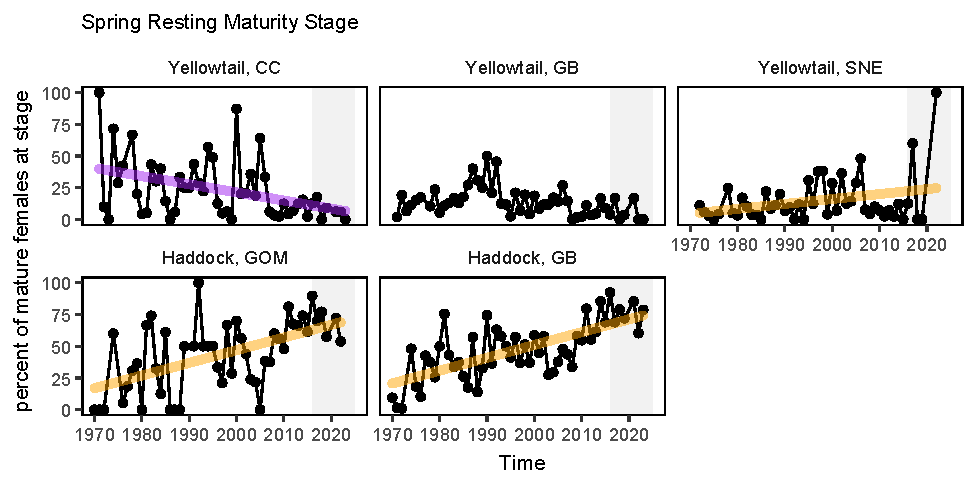
\includegraphics{midatlantic_files/figure-latex/spawntiming-1} 

}

\caption{Percent resting stage (non-spawning) mature female fish (black) from spring NEFSC bottom trawl survey with significant increases (orange) and decreases (purple) from two haddock and three yellowtail flounder stocks: CC = Cape Cod Gulf of Maine, GOM = Gulf of Maine, GB = Georges Bank, SNE = Southern New England.}\label{fig:spawntiming}
\end{figure}

\href{https://noaa-edab.github.io/catalog/timing_shifts.html}{Migration timing} of some tuna and large whale migrations has changed. An analysis of recreational fishing data between 2019 and 2022 identified multiple shifts in important HMS species. For example, Bigeye tuna were caught 50 days earlier; small and large bluefin tuna were caught 38 and 80 days earlier respectively in Massachusetts; and blue marlin in New York were caught 27 days earlier. In Cape Cod Bay, peak spring habitat use by right and humpback whales has shifted 18-19 days later over time.

Understanding whether seasonal patterns are changing for stocks requires regular observations throughout the year. For example, baseline work on \href{https://noaa-edab.github.io/catalog/cetacean_acoustic.html}{cetacean presence in Southern New England} shows different seasonal use patterns for whale and dolphin species. Despite the importance of understanding seasonal patterns, we have few indicators that directly assess timing shifts of species. We plan on incorporating more indicators of timing shifts and phenology in future reports.

\paragraph{Drivers:}\label{drivers-1}

The drivers of timing shifts in managed stocks are generally coupled to shifts in environmental or biological conditions, since these can result in changes in habitat quality or food availability within the year. Changes in the timing of fall phytoplankton blooms and seasonal shifts in zooplankton communities are indicators of changes in seasonal food availability to stocks.

Along with the overall warming trends in the Mid-Atlantic Bight, ocean summer conditions have been lasting longer (Fig. \ref{fig:transition}) due to the later \href{https://noaa-edab.github.io/catalog/trans_dates.html}{transition} from warm summer conditions to cooler fall temperatures. These transition dates relate how daily temperatures compare to the seasonal norm. Changes in the timing of seasonal environmental cycles can alter biological processes (migrations, spawning, etc.) that are triggered by seasonal events.

\begin{figure}

{\centering 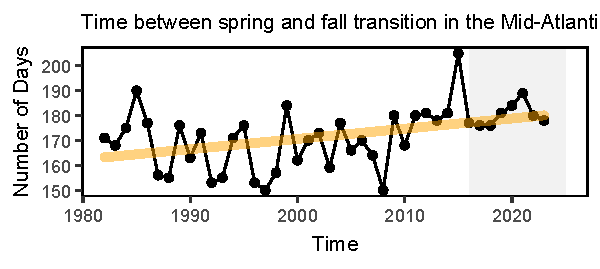
\includegraphics{midatlantic_files/figure-latex/transition-1} 

}

\caption{Ocean summer length in the MAB: the annual total number of days between the spring thermal transition date and the fall thermal transition date (black), with an increasing trend (orange).}\label{fig:transition}
\end{figure}

\begin{verbatim}
## [1] "Beginning 06_risk_seasonal_midatlantic.Rmd"
\end{verbatim}

As noted above, the Middle Atlantic \href{https://noaa-edab.github.io/catalog/cold_pool.html}{Cold Pool} is a summer to early fall feature that creates seasonally suitable habitat for some species. Cold pool persistence, a measure of how long this feature is present in a given year, has been declining, so this habitat is available for a shorter portion of the year (Fig. \ref{fig:cold-pool-time}). All cold pool indices were near the long-term average in 2024 and likely related to the influx of northern waters into the system (see \hyperref[highlights]{2024 Highlights section}). A change in the timing of the autumn breakdown of the cold pool may impact the recruitment of species that depend on it for habitat, such as juvenile yellowtail flounder.

\begin{figure}

{\centering 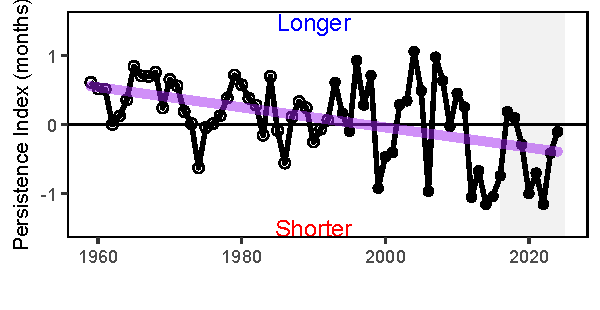
\includegraphics{midatlantic_files/figure-latex/cold-pool-time-1} 

}

\caption{Cold pool persistence index based on bias-corrected ROMS-NWA (open circles) and GLORYS (closed circles).}\label{fig:cold-pool-time}
\end{figure}

The seasonal timing of Mid-Atlantic \href{https://noaa-edab.github.io/catalog/chl_pp.html}{phytoplankton} blooms shows high interannual variability during the fall bloom period (October-December, Fig. \ref{fig:montlychl}). The significant increase in January chlorophyll suggests that the fall bloom period is continuing into the winter, with more chlorophyll now than in the late 1990s. The significant decrease of chlorophyll in September could be related to warmer temperatures persisting into early fall and increased nutrient limitation.

\begin{figure}

{\centering 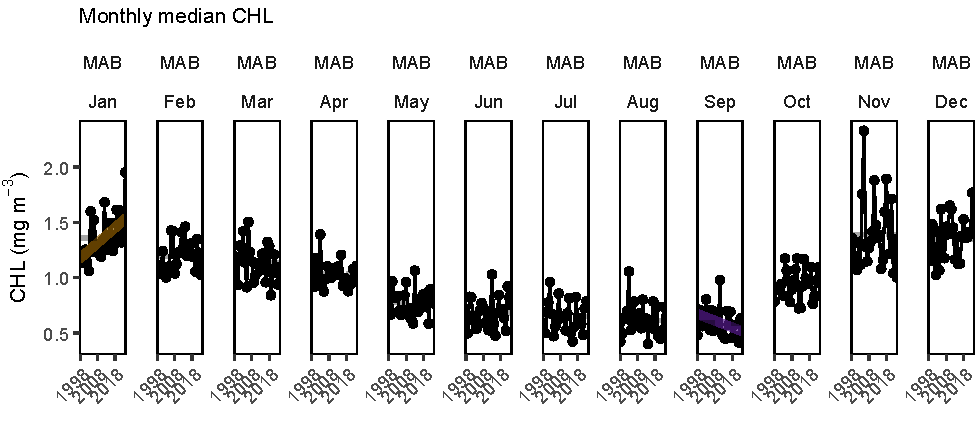
\includegraphics{midatlantic_files/figure-latex/montlychl-1} 

}

\caption{Monthly median chlorophyll a concentration in the MAB (black) with significant increase in January (orange line) and decrease in September (purple line).}\label{fig:montlychl}
\end{figure}

\begin{verbatim}
## [1] "Ending 06_risk_seasonal_midatlantic.Rmd"
\end{verbatim}

\paragraph{Future Considerations}\label{future-considerations-1}

For species reliant on environmental processes to dictate the timing of their behavior (e.g.~phytoplankton bloom timing, thermal transition, or the duration of the cold pool), it is possible that some changes are episodic and have interannual variability, while other timing effects can change on scales of years to decades. Other species may rely on the general seasonal succession of environmental drivers (e.g.~the timing of the fall turnover) to cue biological processes, and these long-term trends are unlikely to reverse in coming years. Such timing shifts in migration or spawning may continue. Management actions that rely on effective alignment of fisheries availability and biological processes should continue to evaluate whether prior assumptions on seasonal timings still hold, and new indicators should be developed to monitor timing shifts for stocks.

\subsubsection{Risks to setting catch limits}\label{risks-to-setting-catch-limits}

The efficacy of short-term stock projections and rebuilding plans rely on accurate understanding of processes affecting stock growth, reproduction, and natural mortality. These biological processes are often driven by underlying environmental change. When observed environmental change occurs, there is a risk that established stock-level biological reference points may no longer reflect the current population and short-term projections become more uncertain.

\begin{verbatim}
## [1] "Beginning 07_risk_setting_catch_limits_midatlantic.Rmd"
\end{verbatim}

\paragraph{Indicators: Fish productivity and condition shifts}\label{indicators-fish-productivity-and-condition-shifts}

Indicators of \href{https://noaa-edab.github.io/catalog/productivity_anomaly.html}{fish productivity} are derived from observations (surveys) or models (stock assessments). Fish productivity has been declining in the Mid-Atlantic since the early 2000s, as described by the small-fish-per-large-fish anomaly indicator (derived from NEFSC bottom trawl survey) (Fig. \ref{fig:productivity-anomaly}). This decline in fish productivity is also shown by a similar analysis based on stock assessment model outputs (recruitment per spawning stock biomass anomaly).

\begin{figure}

{\centering 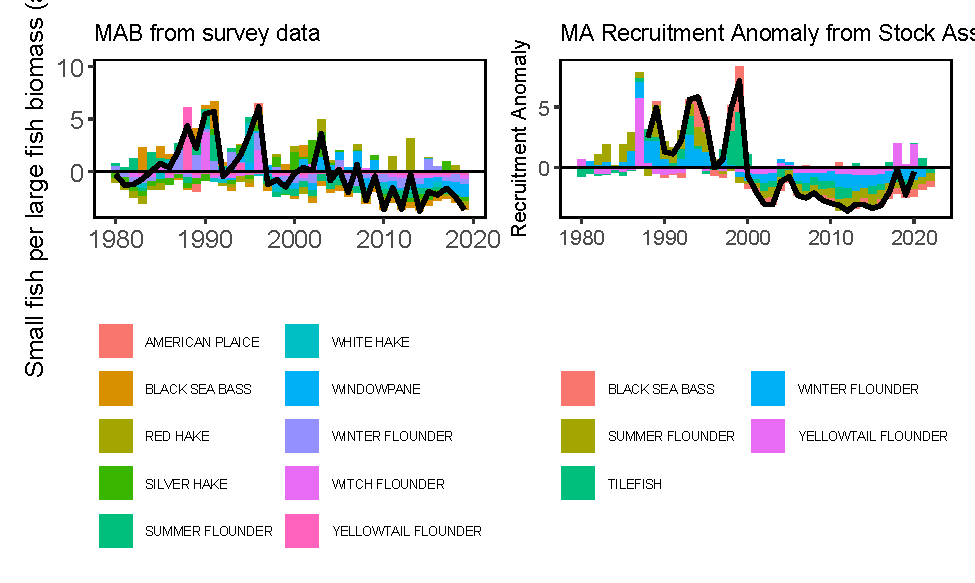
\includegraphics{midatlantic_files/figure-latex/productivity-anomaly-1} 

}

\caption{Fish productivity measures. Left: Small fish per large fish survey biomass anomaly in the Mid-Atlantic Bight. Right: assessment recruitment per spawning stock biomass anomaly for stocks mainly in the Mid-Atlantic. The summed anomaly across species is shown by the black line, drawn across all years with the same number of stocks analyzed.}\label{fig:productivity-anomaly}
\end{figure}

The health of individual fish (i.e.~fish condition, measured as weight for a given length) can contribute to population productivity through improved growth, reproduction and survival. \href{https://noaa-edab.github.io/catalog/condition.html}{Fish condition} in the MAB was generally good prior to 2000, poor from 2001-2010 (concurrent with declines in productivity, Fig. \ref{fig:productivity-anomaly}), and a mix of good and poor since 2011. In 2024, condition continued to be mixed, with general improvement since a relatively low condition year in 2021 (Fig. \ref{fig:mab-cf}). Preliminary analyses show that changes in temperature, zooplankton, fishing pressure, and population size influence the condition of different fish species.

\begin{figure}

{\centering 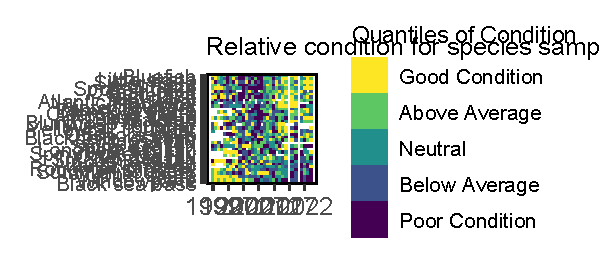
\includegraphics{midatlantic_files/figure-latex/mab-cf-1} 

}

\caption{Condition factor for fish species in the MAB based on fall NEFSC bottom trawl survey data. MAB data are missing for 2017 due to survey delays, and no survey was conducted in 2020.}\label{fig:mab-cf}
\end{figure}

\paragraph{Drivers:}\label{drivers-2}

Fish productivity and condition are affected by increasing metabolic demands from increasing temperature, combined with changes in the availability and quality of prey. Long-term environmental trends and episodic extreme temperatures, ocean acidification, and low oxygen events represent multiple stressors that can affect growth rates, reproductive success, recruitment, and cause mortality.

\subparagraph{Biological Drivers: Forage quality and abundance}\label{biological-drivers-forage-quality-and-abundance}

The amount of forage fish available in the ecosystem combined with the energy content of the forage species determines the amount of energy potentially available to predators in the ecosystem. Changes in the forage base can drive managed and protected species production.

The \href{https://noaa-edab.github.io/catalog/energy_density.html}{energy content} of juvenile and adult forage fish as prey is related to forage fish growth and reproductive cycles, as well as environmental conditions. The energy content of Atlantic herring was estimated to be highest of any forage species in the 1980s and 1990s, based on very small numbers of fish. Most observations from the NEFSC trawl surveys are below the previous estimates (Fig. \ref{fig:energy-density}). However, a recent study that included samples from additional sources indicated herring energy density peaked in summer, with some values closer to the historic estimates. Silver hake, longfin squid (\emph{Loligo} in figure) and shortfin squid (\emph{Illex} in figure) remain lower than previous estimates.

\begin{figure}

{\centering 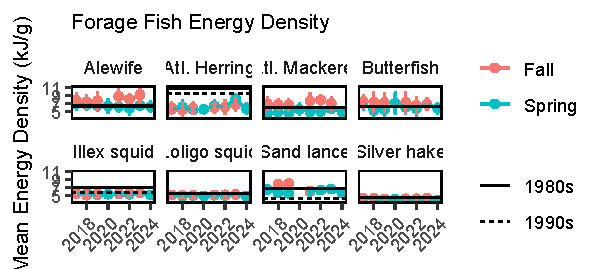
\includegraphics{midatlantic_files/figure-latex/energy-density-1} 

}

\caption{Energy density (mean and standard deviation) of eight forage species from NEFSC bottom trawl surveys by season and year, compared with limited data available from the 1980s (solid line) and 1990s (dashed line)}\label{fig:energy-density}
\end{figure}

Changes in the overall abundance of forage fish can influence managed species productivity as it relates to changes in food availability. A spatially-explicit \href{https://noaa-edab.github.io/catalog/forage_index.html}{forage index} for the Mid-Atlantic shows a long term declining trend in fall, with higher forage biomass in fall than spring (Fig. \ref{fig:foragebio}). Forage biomass was highest during fall in the early-1980s.

\begin{figure}

{\centering 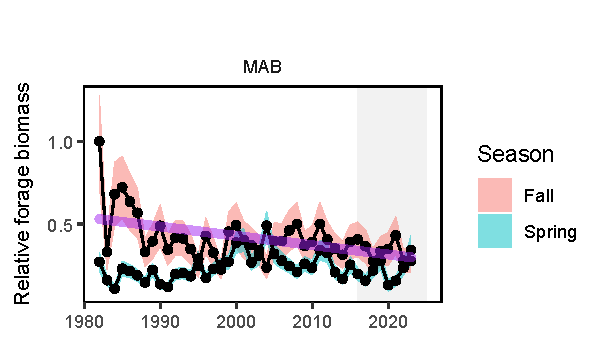
\includegraphics{midatlantic_files/figure-latex/foragebio-1} 

}

\caption{Forage fish index in the MAB for spring (blue) and fall (red) surveys, with a decline (purple) in fall. Index values are relative to the maximum observation within a region across surveys.}\label{fig:foragebio}
\end{figure}

\href{https://noaa-edab.github.io/catalog/benthos_index.html}{Benthic invertebrates} are extremely important forage for some managed species (black sea bass, yellowtail and winter flounders, Atlantic cod, and haddock, and many skate species). Macrobenthos indices show long term declines in spring (Fig. \ref{fig:benthos}). In contrast, megabenthos indices show long-term increases in spring in the MAB.

\begin{figure}

{\centering 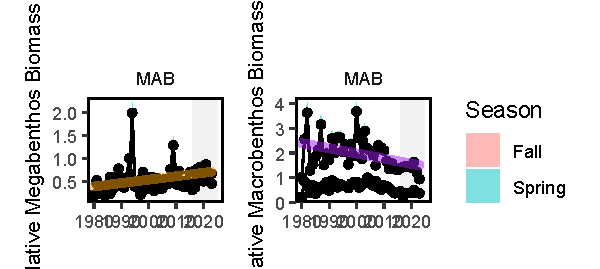
\includegraphics{midatlantic_files/figure-latex/benthos-1} 

}

\caption{Changes in spring (blue) and fall (red) benthos abundance in the MAB for megabenthos (left) and macrobenthos (right).}\label{fig:benthos}
\end{figure}

\subparagraph{Biological Drivers: Lower trophic levels}\label{biological-drivers-lower-trophic-levels}

\href{https://noaa-edab.github.io/catalog/chl_pp.html}{Phytoplankton} are the foundation of the food web and are the primary food source for zooplankton and filter feeders such as shellfish. Multiple environmental and oceanographic drivers affect the abundance, \href{https://noaa-edab.github.io/catalog/chl_pp.html}{composition}, spatial distribution, and productivity of phytoplankton. While changes in phytoplankton productivity could affect fish productivity (including forage), there is no clear long-term trend in Mid-Atlantic total primary production (Fig. \ref{fig:totpp}).

\href{https://noaa-edab.github.io/catalog/zoo_abundance_anom.html}{Zooplankton} communities in the Mid-Atlantic have high variability without trend for large copepods (Fig. \ref{fig:zoopanom}), long term and recent decreasing trends for smaller bodied copepods, and increasing trends for krill (Euphausiids). Small copepods are less energy-rich than Euphausiids (krill) or the larger-bodied copepod \emph{Calanus finmarchicus}. A changing mix of zooplankton prey can impact forage fish energy content and abundance, as well as the prey field of filter feeding whales.

\begin{figure}

{\centering 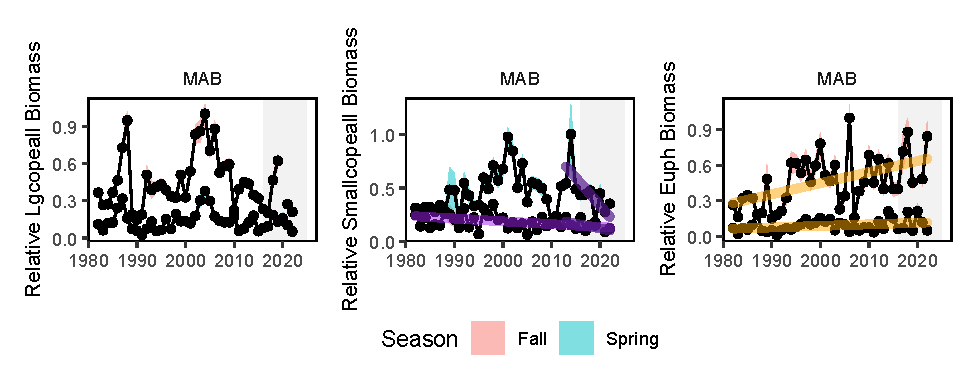
\includegraphics{midatlantic_files/figure-latex/zoopanom-1} 

}

\caption{Changes in zooplankton abundance in the MAB for large (left) and small (center) copepods, and Euphausiids (right), with significant decreases (purple) in small copepods and increases (orange) in Euphausiids.}\label{fig:zoopanom}
\end{figure}

\subparagraph{Environmental Drivers}\label{environmental-drivers}

Fish production can also be directly related to the prevailing environmental conditions by altering metabolic (growth) and reproductive processes. Many species possess thermal tolerances and can experience stressful or lethal conditions if temperatures exceed certain levels. Extreme temperatures at both the \href{https://noaa-edab.github.io/catalog/seasonal_oisst_anom.html}{surface} and \href{https://noaa-edab.github.io/catalog/bottom_temp_model_anom.html}{bottom} can exceed \href{https://noaa-edab.github.io/catalog/thermal_habitat_gridded.html}{thermal tolerance} limits for some fish, which we have observed in past years. However, in 2024, surface and bottom temperatures were near or below normal in the MAB. The amount of habitat exceeding a 24 C thermal tolerance was limited to the southern MAB and the conditions persisted for fewer than 30 days (Fig. \ref{fig:therm-hab-persist-2024}).

In 2024, there were no \href{https://noaa-edab.github.io/catalog/heatwave.html}{marine heatwaves} in the MAB. Only one marine heatwave occurred throughout the entire U.S. Northeast Shelf due to the cooler ocean conditions observed in the region. This surface marine heatwave occurred in the \href{https://noaa-edab.github.io/catalog/heatwave_year.html\#newengland-22}{Gulf of Maine} starting on May 29th, peaking on June 7th, and lasting 12 days.

\begin{figure}

{\centering 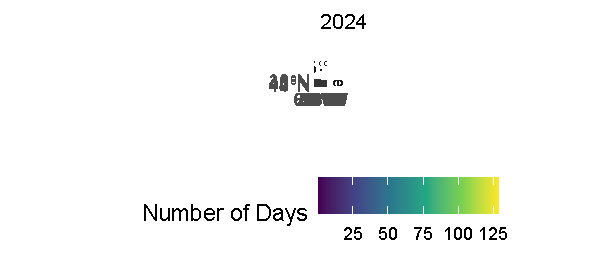
\includegraphics{midatlantic_files/figure-latex/therm-hab-persist-2024-1} 

}

\caption{The number of days in 2024 where bottom temperature exceeds 15℃ (left) and 24℃ (right) based on the GLORYS 1/12 degree grid.}\label{fig:therm-hab-persist-2024}
\end{figure}

\href{https://noaa-edab.github.io/catalog/ocean_acidification.html}{Ocean acidification} risks vary among species and include reduced survival, growth, reproduction, and productivity, where high OA risk indicates potential negative effects to species. OA risk can also be heightened during colder conditions due to increased \(CO_2\) absorption by the water or by transport of high \(CO_2\) water masses (see \hyperref[highlights]{highlights section}). Higher OA risk conditions were observed for Atlantic sea scallop and longfin squid in Long Island Sound and the nearshore and mid shelf regions of the New Jersey shelf during summers of 2016, 2018, 2019, 2023, and 2024 (Fig. \ref{fig:mab-oa}). The OA indicator observed on the Mid-Atlantic coastal shelf during summer 2024 was the most extreme recorded when compared to all of the years sampled (since 2007).

\begin{figure}

{\centering 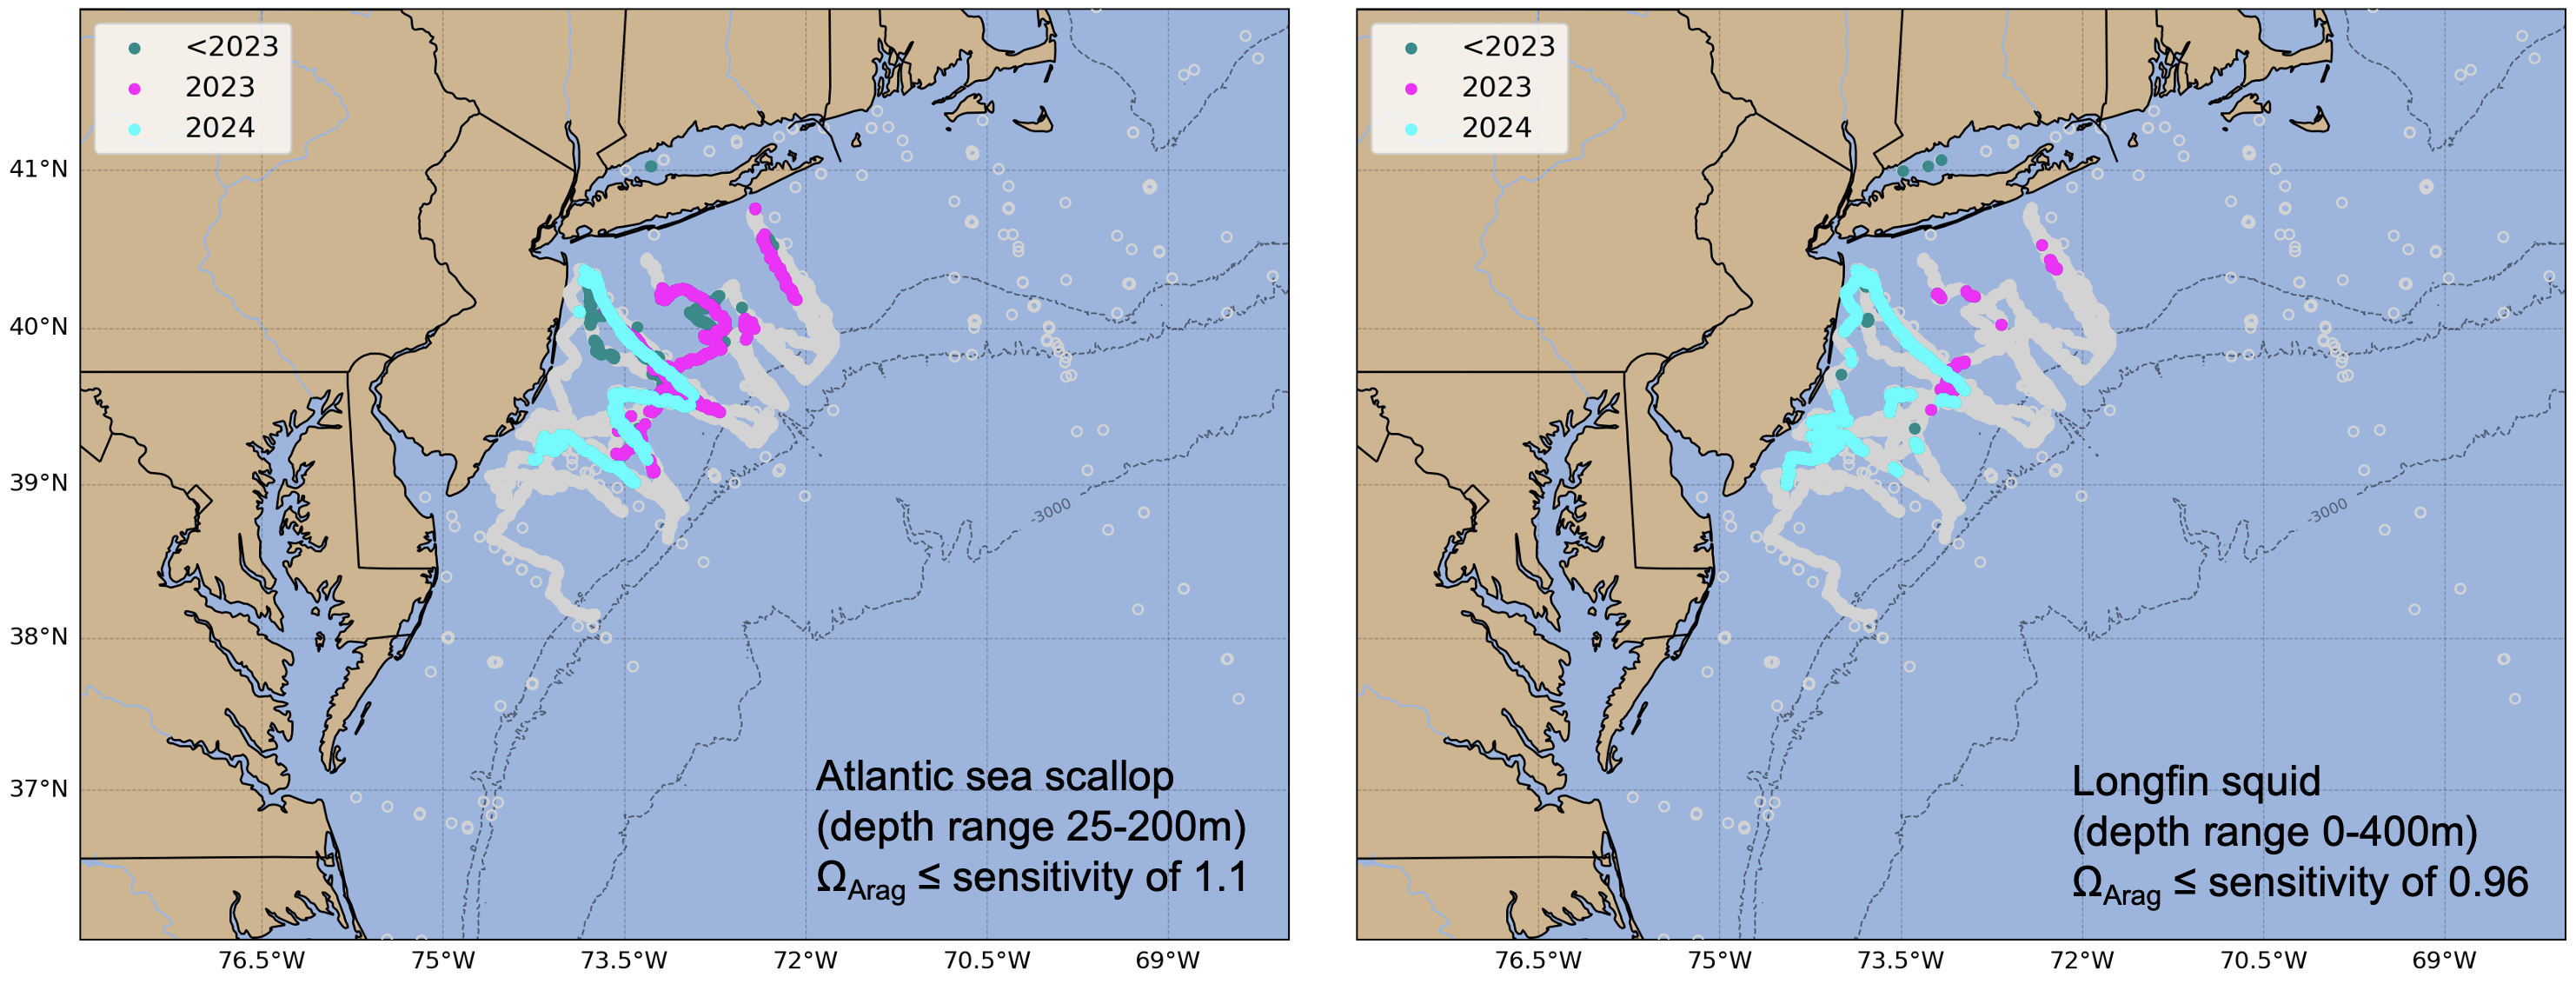
\includegraphics[width=1\linewidth]{images/SOE-2025-OA-figure_final_GraceSaba_2025} 

}

\caption{Locations where bottom aragonite saturation state ($\Omega_{Arag}$; summer only: June-August) were at or below the laboratory-derived sensitivity level for Atlantic sea scallop (left panel) and longfin squid (right panel) for the time periods 2007-2022 (dark cyan), 2023 only (magenta) and 2024 only (cyan). Gray circles indicate locations where bottom $\Omega_{Arag}$ values were above the species specific sensitivity values..}\label{fig:mab-oa-1}
\end{figure}

Low oxygen was detected on the \href{https://noaa-edab.github.io/catalog/observation_synthesis_2023.html}{MAB shelf in 2023}, but not in 2024. Biological and oceanographic processes can affect the amount of oxygen present in the water column. During low oxygen (hypoxic) events, species growth is negatively affected, and very low oxygen can result in \href{https://sebsnjaesnews.rutgers.edu/2023/12/rutgers-scientists-observe-unusual-ocean-conditions-possibly-linked-to-mortality-in-marine-life-off-new-jersey/}{mortality}.

\subparagraph{Drivers: Predation}\label{drivers-predation}

The abundance and distribution of marine mammal, HMS, and shark predators can affect both the productivity and mortality rates on managed stocks. Predators can consume managed species or compete for the same resources, resulting in increased natural mortality or decreased productivity. The northeast shift in \href{https://noaa-edab.github.io/catalog/cetacean_dist.html}{whales and dolphins} (Fig. \ref{fig:protectedspp-dist-shifts}) indicates a change in the overlap between predators and prey. Since we also observe distribution shifts in managed species as well as forage species, the effect of changing predator distributions alone is difficult to quantify.

Indicators for shark populations, combined with information on gray seals (see \hyperref[protected-species]{Protected Species Implications section, above}), suggests predator populations range from stable (\href{https://noaa-edab.github.io/catalog/hms_cpue.html}{sharks}) to increasing (\href{https://noaa-edab.github.io/catalog/seal_pups.html}{gray seals}) in the MAB. \href{https://noaa-edab.github.io/catalog/hms_stock_status.html}{Stock status} is mixed for Atlantic Highly Migratory Species (HMS) stocks (including sharks, swordfish, billfish, and tunas) occurring throughout the Northeast U.S. shelf. While there are several HMS species considered to be overfished or that have unknown stock status, the population status for some managed Atlantic sharks and tunas is at or above the biomass target, suggesting the potential for robust (or rebuilt) predator populations among these managed species. Stable predator populations suggest stable predation pressure on managed species, but increasing predator populations may reflect increasing predation pressure.

\begin{verbatim}
## [1] "Ending 07_risk_setting_catch_limits_midatlantic.Rmd"
\end{verbatim}

\paragraph{Future Considerations}\label{future-considerations-2}

The processes that control fish productivity and mortality are dynamic, complex, and are the result of the interactions between multiple system drivers. There is a real risk that short-term predictions in assessments and rebuilding plans that assume unchanging underlying conditions will be highly uncertain and not be as effective, given the observed change documented in the prior sections in both ecological and environmental processes. Assumptions for species' growth, reproduction, and natural mortality should continue to be evaluated for individual species. With observations of system-wide productivity shifts of multiple managed stocks, more research is needed to determine whether regime shifts or ecosystem reorganization are occurring, and how this should be incorporated into management.

\subsection{Other Ocean Uses: Offshore Wind}\label{other-ocean-uses-offshore-wind}

\subsubsection{Indicators: development timeline, revenue in lease areas, coastal community vulnerability}\label{indicators-development-timeline-revenue-in-lease-areas-coastal-community-vulnerability}

All reported potential offshore wind projected development timelines and data are subject to change and have been based on BOEM Environmental Impact Statements. Offshore wind development schedule and areas are subject to change based on the Executive Order \href{https://www.whitehouse.gov/presidential-actions/2025/01/temporary-withdrawal-of-all-areas-on-the-outer-continental-shelf-from-offshore-wind-leasing-and-review-of-the-federal-governments-leasing-and-permitting-practices-for-wind-projects/}{Temporary Withdrawal of All Areas on the Outer Continental Shelf from Offshore Wind Leasing and Review of the Federal Government's Leasing and Permitting Practices for Wind Projects}.

As of January 2025, 30 offshore \href{https://noaa-edab.github.io/catalog/wind_dev_speed.html}{wind development} projects are proposed for construction over the next decade in the Northeast (timelines and project data for 2025 are based on the Maryland Offshore Wind Final Environmental Impact Statement, Appendix D). Offshore wind areas are anticipated to cover more than 2.3 million acres by 2030 in the Greater Atlantic region (Fig. \ref{fig:wind-proposed-dev}). An additional 800,000 lease acres are proposed for development beyond 2030 and 17 million acres are identified by BOEM as designated planning areas (Fig. \ref{fig:wind-dev-cumul}).

\begin{figure}

{\centering 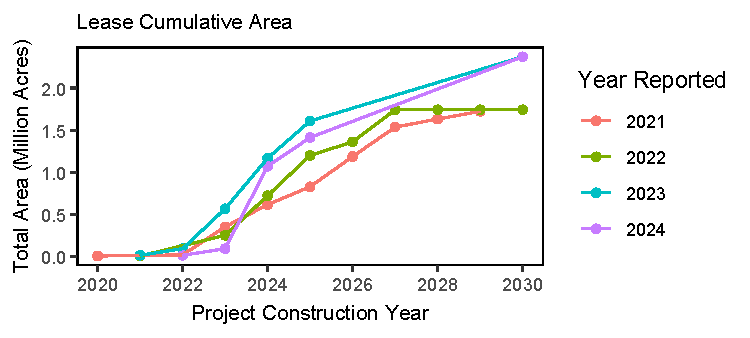
\includegraphics{midatlantic_files/figure-latex/wind-proposed-dev-1} 

}

\caption{Total area proposed for wind develpment on the northeast shelf through 2030.}\label{fig:wind-proposed-dev}
\end{figure}

Just over 3,200 foundations and more than 12,000 miles of inter-array and offshore export cables are proposed to date (Fig. \ref{fig:wind-dev-cumul}). Based on current timelines, the areas affected would be spread out such that it is unlikely that any one region would experience full development at one time. Construction of three projects in Southern New England (Vineyard Wind, South Fork Wind Farm, and Revolution Wind) and two more in the Mid-Atlantic/New York Bight (Coastal Virginia Offshore Wind and Empire Wind 1) during 2024 affected fisheries managed by the Mid-Atlantic Fishery Management Council. It is likely that construction will begin on other projects in Southern New England and possibly the New York Bight during 2025 that will further affect regional fisheries.

\begin{figure}

{\centering 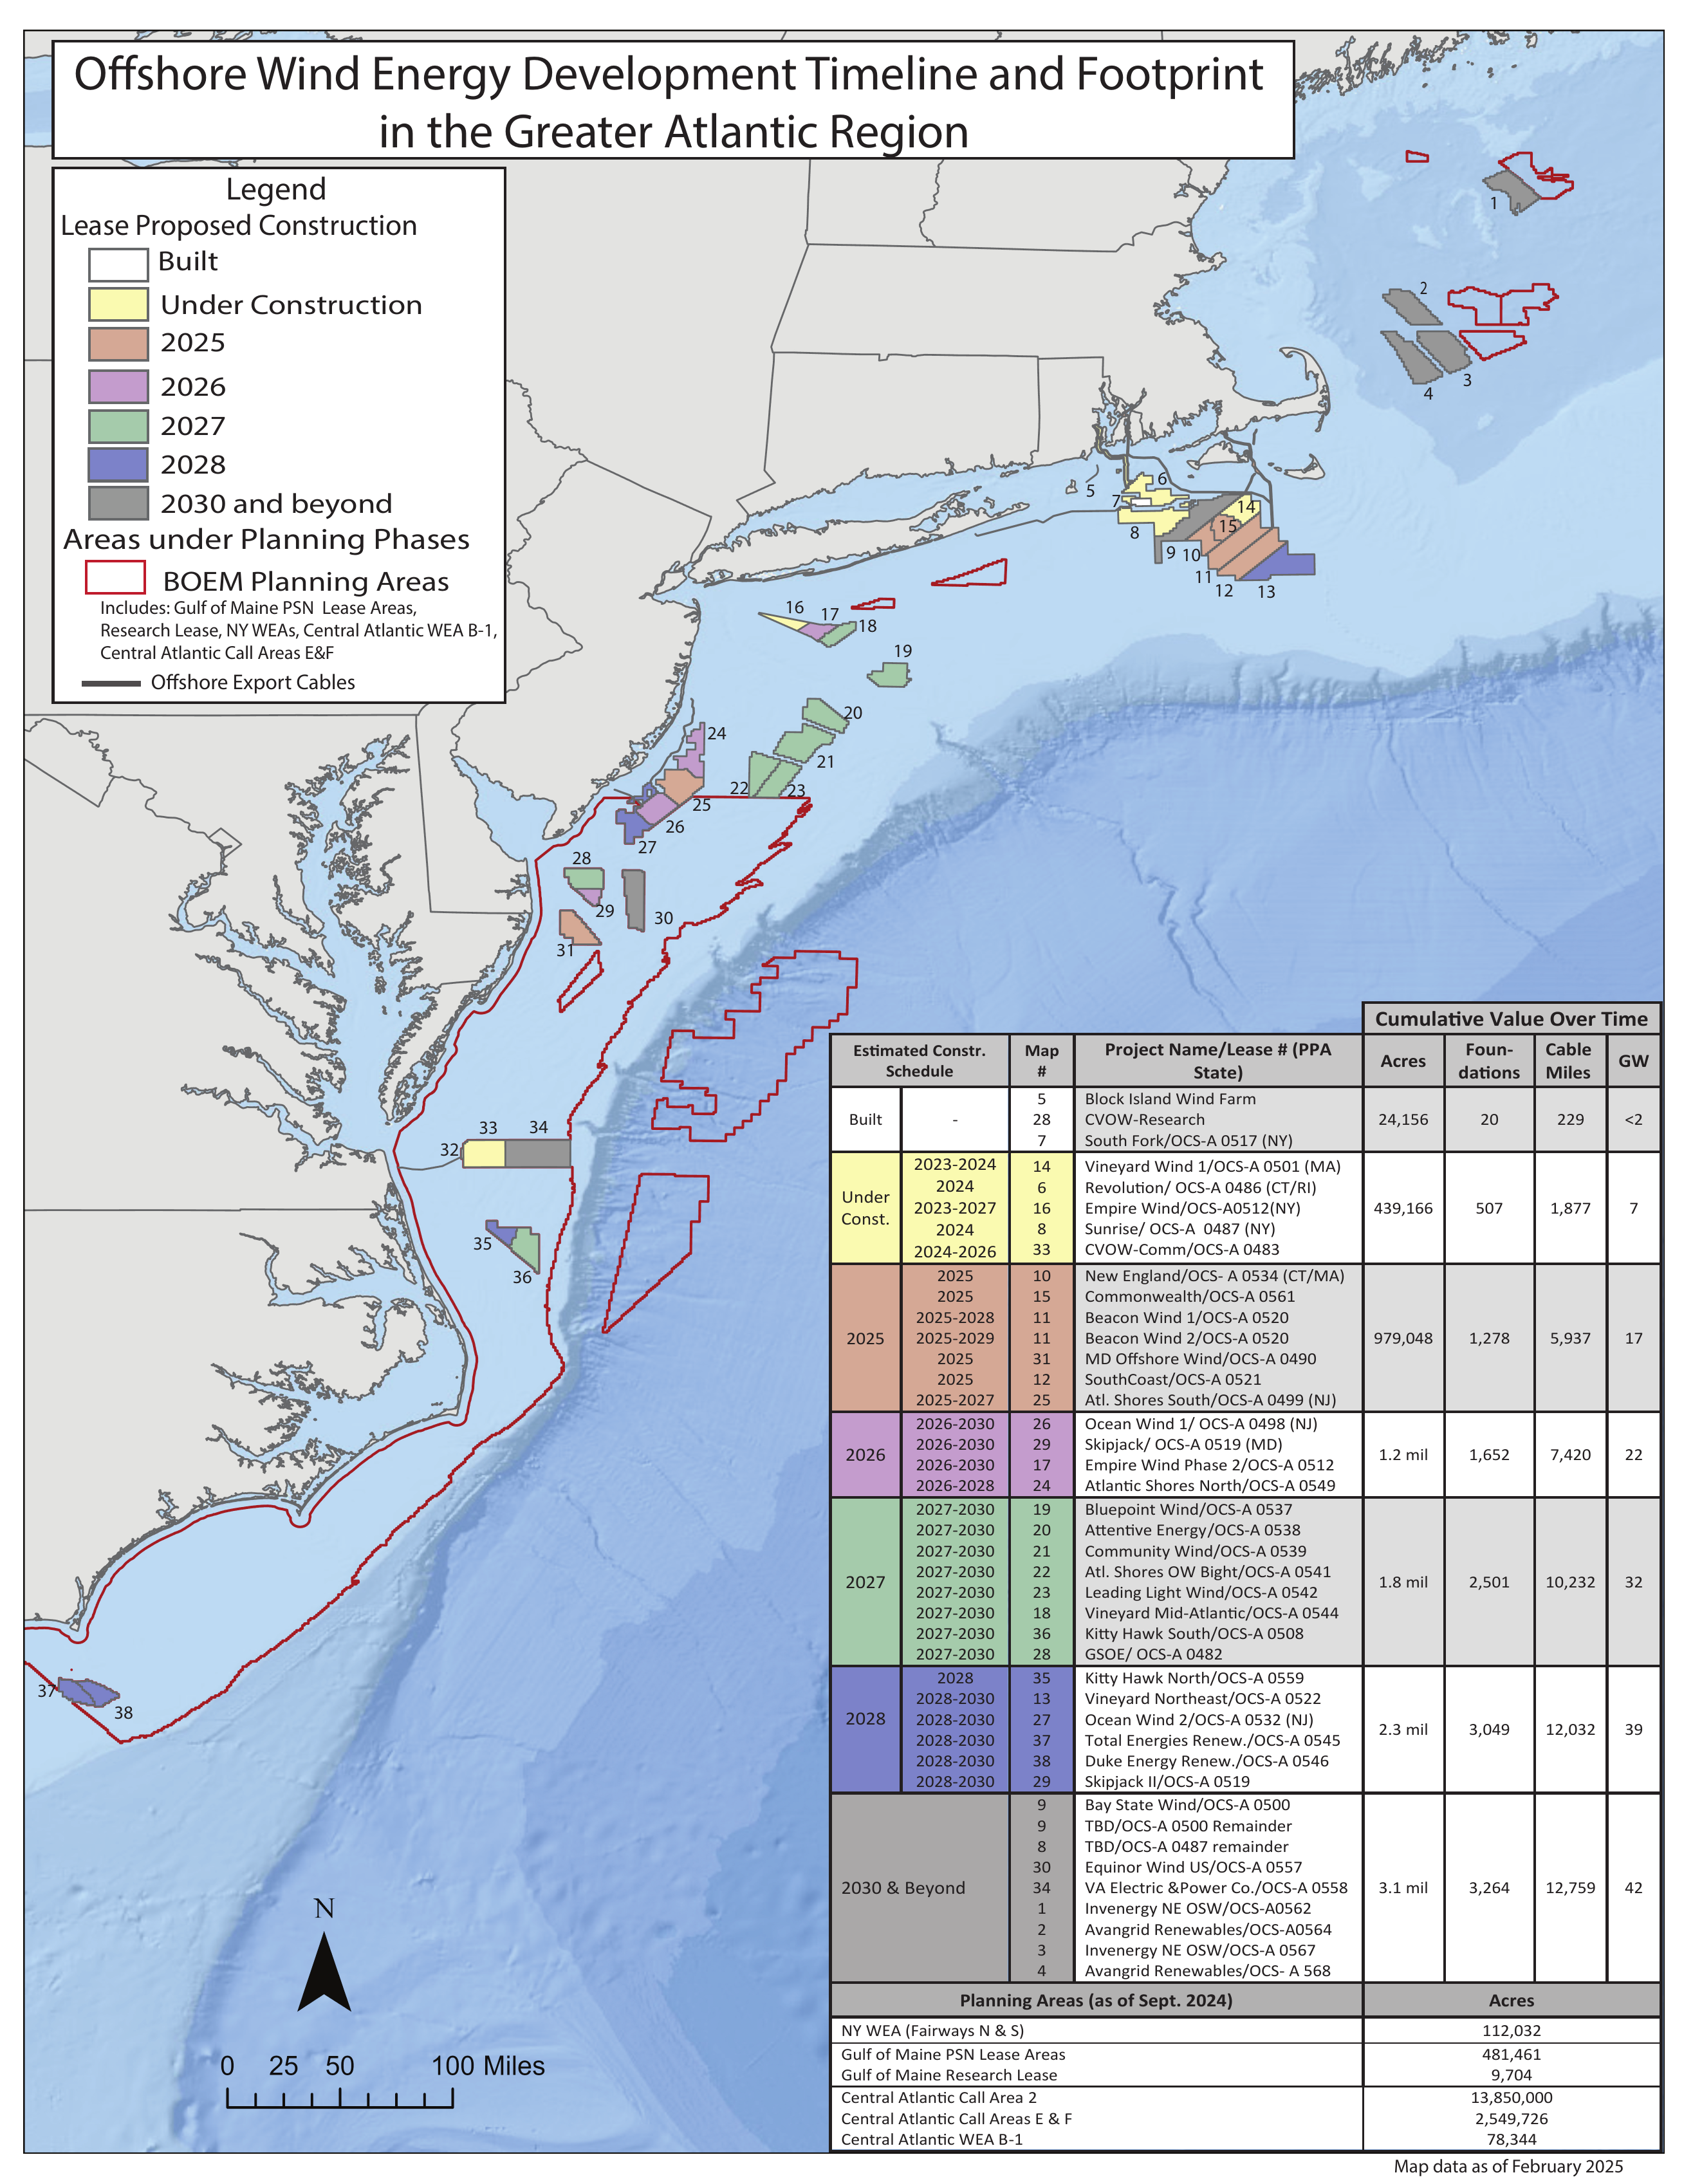
\includegraphics[width=0.9\linewidth]{midatlantic_files/figure-latex/wind-dev-cumul-1} 

}

\caption{All Northeast Project areas by year construction ends (each project has a 2 year construction period).}\label{fig:wind-dev-cumul}
\end{figure}

\begin{verbatim}
## [1] "Beginning 08_offshore_wind_midatlantic.Rmd"
\end{verbatim}

Based on federal vessel logbook data, \href{https://noaa-edab.github.io/catalog/wind_revenue.html}{commercial fishery revenue} from trips in the current offshore wind lease areas, including the newly designated lease areas in the Central Atlantic, have varied annually from 2008-2023, with less than \$1 million in maximum annual revenue overlapping with these areas for most fisheries with the exception of the surfclam, monkfish, and longfin squid fisheries. Some fisheries see periodic spikes in revenue overlap with wind energy lease areas, including the surfclam (\$6.5 million), longfin squid (\$4.8 million), monkfish (\$2.5 million), and summer flounder (\$1.3 million) fisheries (Fig. \ref{fig:wea-spp-rev}).

\begin{figure}

{\centering 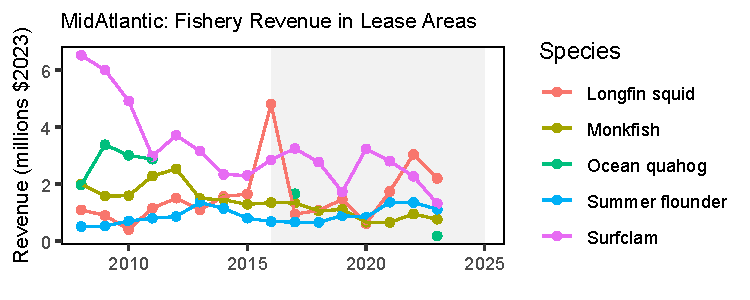
\includegraphics{midatlantic_files/figure-latex/wea-spp-rev-1} 

}

\caption{Fishery revenue in wind energy lease areas in the Mid-Atlantic.}\label{fig:wea-spp-rev}
\end{figure}

Of MAFMC managed fisheries, the surfclam fishery would be the most affected by offshore wind development, with a maximum of 15\% of annual regional fishery revenue occurring within existing wind lease areas during 2008-2023 (see Table \ref{tab:wea-landings-rev-1}). It should be noted that 2023 surfclam landings/revenue within lease areas may be artificially low due to potential misreporting issues. Future fishery resource overlap with wind leases, especially surfclams and ocean quahogs, may change due to species distribution shifts attributable to climate change and recruitment and larval dispersion pattern changes caused by hydrodynamic flow disruptions from turbine foundations, which could also affect fishery landings/revenue.

Offshore wind indicators are based on federal logbook data and do not include all data for all fisheries; therefore a complete evaluation of potential offshore wind energy development impacts would need to be supplemented by other data sources. For further information on the utility of the data, see the \href{https://www.fisheries.noaa.gov/resource/data/socioeconomic-impacts-atlantic-offshore-wind-development}{socioeconomic impacts of offshore wind development data reports page}.

\global\setlength{\Oldarrayrulewidth}{\arrayrulewidth}

\global\setlength{\Oldtabcolsep}{\tabcolsep}

\setlength{\tabcolsep}{2pt}

\renewcommand*{\arraystretch}{1}



\providecommand{\ascline}[3]{\noalign{\global\arrayrulewidth #1}\arrayrulecolor[HTML]{#2}\cline{#3}}

\begin{longtable}[c]{|p{2.00in}|p{2.00in}|p{2.00in}}

\caption{Mid-Atlantic\ managed\ species\ Landings\ and\ Revenue\ from\ Wind\ Energy\ Areas.\ *Less\ than\ a\ maximum\ of\ 50,000\ lb\ was\ reported\ landed\ annually\ in\ wind\ energy\ lease\ areas\ for\ these\ species.}\label{tab:wea-landings-rev}\\

\ascline{1.5pt}{666666}{1-3}

\multicolumn{1}{>{\raggedright}m{\dimexpr 2in+0\tabcolsep}}{\textcolor[HTML]{000000}{\fontsize{9}{9}\selectfont{NEFMC,\ MAFMC,\ and\ ASMFC\ Managed\ Species}}} & \multicolumn{1}{>{\raggedleft}m{\dimexpr 2in+0\tabcolsep}}{\textcolor[HTML]{000000}{\fontsize{9}{9}\selectfont{Maximum\ Percent\ Total\ Annual\ Regional\ Species\ Landings}}} & \multicolumn{1}{>{\raggedleft}m{\dimexpr 2in+0\tabcolsep}}{\textcolor[HTML]{000000}{\fontsize{9}{9}\selectfont{Maximum\ Percent\ Total\ Annual\ Regional\ Species\ Revenue}}} \\

\ascline{1.5pt}{666666}{1-3}\endfirsthead \caption[]{Mid-Atlantic\ managed\ species\ Landings\ and\ Revenue\ from\ Wind\ Energy\ Areas.\ *Less\ than\ a\ maximum\ of\ 50,000\ lb\ was\ reported\ landed\ annually\ in\ wind\ energy\ lease\ areas\ for\ these\ species.}\label{tab:wea-landings-rev}\\

\ascline{1.5pt}{666666}{1-3}

\multicolumn{1}{>{\raggedright}m{\dimexpr 2in+0\tabcolsep}}{\textcolor[HTML]{000000}{\fontsize{9}{9}\selectfont{NEFMC,\ MAFMC,\ and\ ASMFC\ Managed\ Species}}} & \multicolumn{1}{>{\raggedleft}m{\dimexpr 2in+0\tabcolsep}}{\textcolor[HTML]{000000}{\fontsize{9}{9}\selectfont{Maximum\ Percent\ Total\ Annual\ Regional\ Species\ Landings}}} & \multicolumn{1}{>{\raggedleft}m{\dimexpr 2in+0\tabcolsep}}{\textcolor[HTML]{000000}{\fontsize{9}{9}\selectfont{Maximum\ Percent\ Total\ Annual\ Regional\ Species\ Revenue}}} \\

\ascline{1.5pt}{666666}{1-3}\endhead



\multicolumn{1}{>{\raggedright}m{\dimexpr 2in+0\tabcolsep}}{\textcolor[HTML]{000000}{\fontsize{9}{9}\selectfont{Blueline\ Tilefish*}}} & \multicolumn{1}{>{\raggedleft}m{\dimexpr 2in+0\tabcolsep}}{\textcolor[HTML]{000000}{\fontsize{9}{9}\selectfont{13}}} & \multicolumn{1}{>{\raggedleft}m{\dimexpr 2in+0\tabcolsep}}{\textcolor[HTML]{000000}{\fontsize{9}{9}\selectfont{16}}} \\





\multicolumn{1}{>{\raggedright}m{\dimexpr 2in+0\tabcolsep}}{\textcolor[HTML]{000000}{\fontsize{9}{9}\selectfont{Atlantic\ Surfclam}}} & \multicolumn{1}{>{\raggedleft}m{\dimexpr 2in+0\tabcolsep}}{\textcolor[HTML]{000000}{\fontsize{9}{9}\selectfont{16}}} & \multicolumn{1}{>{\raggedleft}m{\dimexpr 2in+0\tabcolsep}}{\textcolor[HTML]{000000}{\fontsize{9}{9}\selectfont{15}}} \\





\multicolumn{1}{>{\raggedright}m{\dimexpr 2in+0\tabcolsep}}{\textcolor[HTML]{000000}{\fontsize{9}{9}\selectfont{Ocean\ Quahog}}} & \multicolumn{1}{>{\raggedleft}m{\dimexpr 2in+0\tabcolsep}}{\textcolor[HTML]{000000}{\fontsize{9}{9}\selectfont{12}}} & \multicolumn{1}{>{\raggedleft}m{\dimexpr 2in+0\tabcolsep}}{\textcolor[HTML]{000000}{\fontsize{9}{9}\selectfont{11}}} \\





\multicolumn{1}{>{\raggedright}m{\dimexpr 2in+0\tabcolsep}}{\textcolor[HTML]{000000}{\fontsize{9}{9}\selectfont{Black\ Sea\ Bass}}} & \multicolumn{1}{>{\raggedleft}m{\dimexpr 2in+0\tabcolsep}}{\textcolor[HTML]{000000}{\fontsize{9}{9}\selectfont{9}}} & \multicolumn{1}{>{\raggedleft}m{\dimexpr 2in+0\tabcolsep}}{\textcolor[HTML]{000000}{\fontsize{9}{9}\selectfont{10}}} \\





\multicolumn{1}{>{\raggedright}m{\dimexpr 2in+0\tabcolsep}}{\textcolor[HTML]{000000}{\fontsize{9}{9}\selectfont{Scup}}} & \multicolumn{1}{>{\raggedleft}m{\dimexpr 2in+0\tabcolsep}}{\textcolor[HTML]{000000}{\fontsize{9}{9}\selectfont{8}}} & \multicolumn{1}{>{\raggedleft}m{\dimexpr 2in+0\tabcolsep}}{\textcolor[HTML]{000000}{\fontsize{9}{9}\selectfont{9}}} \\





\multicolumn{1}{>{\raggedright}m{\dimexpr 2in+0\tabcolsep}}{\textcolor[HTML]{000000}{\fontsize{9}{9}\selectfont{Atlantic\ Mackerel}}} & \multicolumn{1}{>{\raggedleft}m{\dimexpr 2in+0\tabcolsep}}{\textcolor[HTML]{000000}{\fontsize{9}{9}\selectfont{8}}} & \multicolumn{1}{>{\raggedleft}m{\dimexpr 2in+0\tabcolsep}}{\textcolor[HTML]{000000}{\fontsize{9}{9}\selectfont{8}}} \\





\multicolumn{1}{>{\raggedright}m{\dimexpr 2in+0\tabcolsep}}{\textcolor[HTML]{000000}{\fontsize{9}{9}\selectfont{Chub\ Mackerel}}} & \multicolumn{1}{>{\raggedleft}m{\dimexpr 2in+0\tabcolsep}}{\textcolor[HTML]{000000}{\fontsize{9}{9}\selectfont{15}}} & \multicolumn{1}{>{\raggedleft}m{\dimexpr 2in+0\tabcolsep}}{\textcolor[HTML]{000000}{\fontsize{9}{9}\selectfont{8}}} \\





\multicolumn{1}{>{\raggedright}m{\dimexpr 2in+0\tabcolsep}}{\textcolor[HTML]{000000}{\fontsize{9}{9}\selectfont{Longfin\ Squid}}} & \multicolumn{1}{>{\raggedleft}m{\dimexpr 2in+0\tabcolsep}}{\textcolor[HTML]{000000}{\fontsize{9}{9}\selectfont{8}}} & \multicolumn{1}{>{\raggedleft}m{\dimexpr 2in+0\tabcolsep}}{\textcolor[HTML]{000000}{\fontsize{9}{9}\selectfont{8}}} \\





\multicolumn{1}{>{\raggedright}m{\dimexpr 2in+0\tabcolsep}}{\textcolor[HTML]{000000}{\fontsize{9}{9}\selectfont{Monkfish}}} & \multicolumn{1}{>{\raggedleft}m{\dimexpr 2in+0\tabcolsep}}{\textcolor[HTML]{000000}{\fontsize{9}{9}\selectfont{9}}} & \multicolumn{1}{>{\raggedleft}m{\dimexpr 2in+0\tabcolsep}}{\textcolor[HTML]{000000}{\fontsize{9}{9}\selectfont{8}}} \\





\multicolumn{1}{>{\raggedright}m{\dimexpr 2in+0\tabcolsep}}{\textcolor[HTML]{000000}{\fontsize{9}{9}\selectfont{Butterfish}}} & \multicolumn{1}{>{\raggedleft}m{\dimexpr 2in+0\tabcolsep}}{\textcolor[HTML]{000000}{\fontsize{9}{9}\selectfont{8}}} & \multicolumn{1}{>{\raggedleft}m{\dimexpr 2in+0\tabcolsep}}{\textcolor[HTML]{000000}{\fontsize{9}{9}\selectfont{7}}} \\





\multicolumn{1}{>{\raggedright}m{\dimexpr 2in+0\tabcolsep}}{\textcolor[HTML]{000000}{\fontsize{9}{9}\selectfont{Golden\ Tilefish}}} & \multicolumn{1}{>{\raggedleft}m{\dimexpr 2in+0\tabcolsep}}{\textcolor[HTML]{000000}{\fontsize{9}{9}\selectfont{6}}} & \multicolumn{1}{>{\raggedleft}m{\dimexpr 2in+0\tabcolsep}}{\textcolor[HTML]{000000}{\fontsize{9}{9}\selectfont{6}}} \\





\multicolumn{1}{>{\raggedright}m{\dimexpr 2in+0\tabcolsep}}{\textcolor[HTML]{000000}{\fontsize{9}{9}\selectfont{Summer\ Flounder}}} & \multicolumn{1}{>{\raggedleft}m{\dimexpr 2in+0\tabcolsep}}{\textcolor[HTML]{000000}{\fontsize{9}{9}\selectfont{5}}} & \multicolumn{1}{>{\raggedleft}m{\dimexpr 2in+0\tabcolsep}}{\textcolor[HTML]{000000}{\fontsize{9}{9}\selectfont{5}}} \\





\multicolumn{1}{>{\raggedright}m{\dimexpr 2in+0\tabcolsep}}{\textcolor[HTML]{000000}{\fontsize{9}{9}\selectfont{Bluefish*}}} & \multicolumn{1}{>{\raggedleft}m{\dimexpr 2in+0\tabcolsep}}{\textcolor[HTML]{000000}{\fontsize{9}{9}\selectfont{4}}} & \multicolumn{1}{>{\raggedleft}m{\dimexpr 2in+0\tabcolsep}}{\textcolor[HTML]{000000}{\fontsize{9}{9}\selectfont{4}}} \\





\multicolumn{1}{>{\raggedright}m{\dimexpr 2in+0\tabcolsep}}{\textcolor[HTML]{000000}{\fontsize{9}{9}\selectfont{Spiny\ Dogfish}}} & \multicolumn{1}{>{\raggedleft}m{\dimexpr 2in+0\tabcolsep}}{\textcolor[HTML]{000000}{\fontsize{9}{9}\selectfont{2}}} & \multicolumn{1}{>{\raggedleft}m{\dimexpr 2in+0\tabcolsep}}{\textcolor[HTML]{000000}{\fontsize{9}{9}\selectfont{3}}} \\





\multicolumn{1}{>{\raggedright}m{\dimexpr 2in+0\tabcolsep}}{\textcolor[HTML]{000000}{\fontsize{9}{9}\selectfont{Illex\ Squid}}} & \multicolumn{1}{>{\raggedleft}m{\dimexpr 2in+0\tabcolsep}}{\textcolor[HTML]{000000}{\fontsize{9}{9}\selectfont{2}}} & \multicolumn{1}{>{\raggedleft}m{\dimexpr 2in+0\tabcolsep}}{\textcolor[HTML]{000000}{\fontsize{9}{9}\selectfont{2}}} \\

\ascline{1.5pt}{666666}{1-3}



\end{longtable}



\arrayrulecolor[HTML]{000000}

\global\setlength{\arrayrulewidth}{\Oldarrayrulewidth}

\global\setlength{\tabcolsep}{\Oldtabcolsep}

\renewcommand*{\arraystretch}{1}

Proposed wind development areas interact with the region's federal scientific surveys. Scientific surveys are impacted by offshore wind in four ways:
1. Exclusion of NOAA Fisheries' sampling platforms from the wind development area due to operational and safety limitations.
2. Impacts on the random-stratified statistical design that is the basis for scientific assessments, advice, and analyses.
3. Alteration of benthic and pelagic habitats, and airspace in and around the wind energy development, requiring new designs and methods to sample new habitats.
4. Reduced sampling productivity through navigation impacts of wind energy infrastructure on aerial and vessel survey operations.

Increased vessel transit between stations may decrease data collections that are already limited by annual days-at-sea day allocations. The total survey area overlap ranges from 1-70\% for all Greater Atlantic federal surveys as of 2024. Individual survey strata have significant interaction with wind areas, including the sea scallop survey (up to 96\% of individual strata) and the bottom trawl survey (up to 60\% strata overlap). Additionally, up to 50\% of the southern New England North Atlantic right whale survey's area overlaps with proposed project areas and a region-wide survey mitigation program is underway.

The socio-demographic conditions, and resultant vulnerabilities, of some communities may further exacerbate the impacts of offshore wind development in the Northeast such that the impacts of offshore wind development are expected to differentially \href{https://noaa-edab.github.io/catalog/wind_port.html}{impact specific coastal communities} (Fig. \ref{fig:wea-port-rev}). Additionally, impacts of offshore wind development may unevenly affect individual operators, with some permit holders deriving a much higher proportion of revenue from wind areas than the port-based mean.

\begin{figure}

\includegraphics{midatlantic_files/figure-latex/wea-port-rev-1} \hfill{}

\caption{Percent of Mid-Atlantic port revenue from Wind Energy Areas (WEA) in descending order from most to least port revenue from WEA.}\label{fig:wea-port-rev}
\end{figure}

For example, Atlantic City, NJ was in the top three potential revenue loss (historical minimum of 3\% and maximum of 24\%, respectively) from potential wind development areas based on 2008-2023 total port fisheries revenue. BOEM reports that cumulative offshore wind development (if all proposed projects are developed) could have moderate impacts on low-income members of communities with socio-demographic concerns who work in the commercial fishing and for-hire fishing industry due to disruptions to fish populations, restrictions on navigation and increased vessel traffic, as well as existing vulnerabilities of low-income workers to economic impacts.

Some ports in New England land Mid-Atlantic managed species from wind areas as well. For the maximum percent value reported in each New England port, the majority (at least 50\% based on both value and pounds) of those landings were Mid-Atlantic managed species within wind areas for Davisville/North Kingston and Point Judith, RI, and Hyannis and Menemsha, MA (Fig. \ref{fig:wind-rev-NE-MAFMC}).

\begin{figure}

\includegraphics{midatlantic_files/figure-latex/wind-rev-NE-MAFMC-1} \hfill{}

\caption{Percent of New England port revenue with majority MAFMC landings from Wind Energy Areas (WEA) in descending order from most to least port revenue from WEA.}\label{fig:wind-rev-NE-MAFMC}
\end{figure}

Top fishing communities with \href{https://noaa-edab.github.io/catalog/engagement.html}{socio-demographic concerns} (i.e., Atlantic City, NJ, and Hampton Bays, NY) should be considered in decision making to reduce the social and economic impacts and aid in the resilience and adaptive capacity of underserved communities. These are communities where we need to provide further resources to reach underserved and underrepresented groups and create opportunities for and directly involve these groups in the decision-making process.

\begin{verbatim}
## [1] "Ending 08_offshore_wind_midatlantic.Rmd"
\end{verbatim}

\subsubsection{Implications}\label{implications-6}

Current plans for buildout of offshore wind in a patchwork of areas spreads the impacts differentially throughout the region (Fig. \ref{fig:wind-dev-cumul}). Up to 15\% of maximum annual fisheries revenue for major Mid-Atlantic commercial species in lease areas could be forgone or reduced and associated effort displaced if all sites are developed. Displaced fishing effort can alter historic fishing area, timing, and method patterns, which can in turn change habitat, species (managed and protected), and fleet interactions. Several factors, including fishery regulations, fishery availability, and user conflicts affect where, when, and how fishing effort may be displaced, along with impacts to and responses of affected fish species.

Planned development \href{https://noaa-edab.github.io/catalog/persistent_hotspots.html}{overlaps NARW} mother and calf migration corridors and a significant foraging habitat that is used throughout the year (Fig. \ref{fig:whales-wind}). Turbine presence and extraction of energy from the system could alter local oceanography and may affect right whale prey availability. For example, persistent foraging hotspots of right whales and seabirds overlap on Nantucket Shoals, where unique hydrography aggregates enhanced prey densities. Wind leases (OCS-A 0521 and OCS-A 0522) currently intersect these hotspots on the southwestern corner of Nantucket Shoals and a prominent tidal front associated with invertebrate prey swarms important to seabirds and possibly right whales. Proposed wind development areas also bring increased vessel strike risk from construction and operation vessels. In addition, there are a number of potential impacts to whales from pile driving and operational noise such as displacement, increased levels of communication masking, and elevated stress hormones.

\begin{figure}

{\centering \includegraphics[width=0.55\linewidth]{midatlantic_files/figure-latex/whales-wind-1} 

}

\caption{Northern Right Whale persistent hotspots (red shading) and Wind Energy Areas (black outlines).}\label{fig:whales-wind}
\end{figure}

Scientific data collection surveys for ocean and ecosystem conditions, fish, and protected species will be altered, potentially increasing uncertainty for stock assessments and associated management decision making.

The increase of offshore wind development can have both positive (e.g., employment opportunities) and negative (e.g., space-use conflicts) effects. Continued increase in coastal development and gentrification pressure has resulted in loss of fishing infrastructure space within ports. Understanding these existing pressures can allow for avoiding and mitigating negative impacts to our shore support industry and communities dependent on fishing. Some of the communities with the highest fisheries revenue overlap with offshore wind development areas that are also vulnerable to gentrification pressure are Beaufort, NC, and Cape May, Barnegat Light, and Long Beach, NJ.

\newpage

\subsubsection{2024 Highlights}\label{highlights}

This section intends to provide a record of \href{https://noaa-edab.github.io/catalog/observation_synthesis_2024.html}{noteworthy observations reported in 2024} across the Northeast U.S. region. The full ecosystem and fisheries impacts of many of these observations are still to be determined. They should, however, be noted and considered in future analyses and management decisions.

2024 global sea surface and air temperatures exceeded 2023 as the warmest year on record, but colder than average temperatures were observed in the Northeast U.S. Oceanographic and ecological conditions in the Northwest Atlantic were markedly different in 2024 compared to recent years.

\paragraph{Northwest Atlantic Phenomena}\label{northwest-atlantic-phenomena}

Late 2023 and early 2024 observations indicate movement of cooler and fresher water into the Northwest Atlantic, although there are seasonal and local exceptions to this pattern. Anomalously cold (Fig. \ref{fig:slopesea}) and low salinity conditions were recorded throughout the Northeast Shelf and were widespread across the Slope Sea for much of the year. These cooler and fresher conditions are linked to the southward movement of the eastern portion of the \href{https://noaa-edab.github.io/catalog/gsi.html}{Gulf Stream} and possibly an increased influx of Labrador Slope and Scotian Shelf water into the system.

\begin{figure}

{\centering \includegraphics[width=0.65\linewidth]{midatlantic_files/figure-latex/slopesea-1} 

}

\caption{February 2024 sea surface temperature difference compared to the February 2000-2020 long-term mean from the NOAA Advanced Clear-Sky Processor for Ocean (ACSPO) Super-collated SST.}\label{fig:slopesea}
\end{figure}

In 2023, Labrador Slope water accounted for more than 50\% of the \href{https://noaa-edab.github.io/catalog/slopewater.html}{source water} entering the Gulf of Maine through the Northeast Channel (Fig. \ref{fig:slopewater}); data are still being processed for 2024. Colder, fresher water detected deep in the Jordan Basin for the \href{https://noaa-edab.github.io/catalog/observation_synthesis_2024.html}{first half of 2024} suggests an increased influx of Labrador Slope and Scotian Shelf water, which resulted in colder and fresher conditions throughout the Northwest Atlantic and contributed to the increased size and colder temperatures of the Mid-Atlantic \href{https://noaa-edab.github.io/catalog/cold_pool.html}{Cold Pool}.

\begin{figure}

{\centering \includegraphics{midatlantic_files/figure-latex/slopewater-1} 

}

\caption{The proportion of Warm Slope Water (WSW) and Labrador Slope Water (LSW) enter the Gulf of Maine through the Northeast Channel. The orange and teal dashed lines represent the long-term proportion averages for the WSW and LSW respectively.}\label{fig:slopewater}
\end{figure}

\paragraph{Northeast Shelf and Local Phenomena}\label{northeast-shelf-and-local-phenomena}

The influx of the northern waters is likely linked to multiple observations across the Northeast Shelf including the uncommon presence of Arctic \emph{Calanus} zooplankton species in the Gulf of Maine, delayed migration of many species, and redistribution of some species. Several members of the fishing community noted delayed migration of species into typical fishing grounds. In particular, they attributed the delayed migration of longfin squid, black sea bass, and haddock to the cooler water temperatures. Many also reported redistribution of some species. Specifically, pollock, bluefin tuna, Atlantic mackerel, longfin squid, bluefish, and bonito were observed in surprising or unusual locations. Some species, such as Atlantic mackerel, were reported outside of typical fishing grounds and in higher abundance compared to recent years. Anglers also reported good catches of red drum in Chesapeake Bay and record high (since 1995) numbers were observed at Poplar Island survey location.

In the summer, Chesapeake Bay recorded warm temperatures and low bottom water dissolved oxygen that resulted in less than suitable habitat for species such as striped bass and blue crabs. These poor conditions can affect their distribution, growth, and survival. Additionally, lower than average spring and summer salinity negatively impacted oyster hatchery operations and increased the area of available habitat for invasive blue catfish, potentially increasing predation on blue crabs and other important finfish species.

During the summer months there were multiple prolonged upwelling events that brought cold water to the surface off the New Jersey coast. There was also an atypical phytoplankton bloom south of Long Island in late June to early July 2024, possibly linked to an upwelling event (Fig. \ref{fig:cocobloom}). The bloom was dominated by coccolithophores, which have an exoskeleton made up of calcium carbonate plates that can turn the water an opaque turquoise color. Large blooms of coccolithophores are unusual in this region, but they are not considered harmful and are grazed by zooplankton. Additionally, there were observations of multiple whale species aggregating near the Hudson Canyon between May and August.

\begin{figure}

{\centering \includegraphics[width=0.55\linewidth]{midatlantic_files/figure-latex/cocobloom-1} 

}

\caption{An OLCI Sentinel 3A true color image with enhanced contrast captured on July 2, 2024. Coccolithophores shed their coccolith plates during the later stages of the bloom cycle, which results in the milky turquoise water color (Image credit: NOAA STAR, OCView and Ocean Color Science Team).}\label{fig:cocobloom}
\end{figure}

Summer bottom \href{https://noaa-edab.github.io/catalog/ocean_acidification.html}{ocean acidification (OA)} risk in the Mid-Atlantic was the highest recorded since sampling began in 2007. High OA risk is measured as low aragonite saturation state(\(\Omega\)). Similarly, the winter/early spring \href{https://noaa-edab.github.io/catalog/gom_acidification.html}{Gulf of Maine surface OA risk} was significantly above the climatological average and near the sensitivity levels for cod (\(\Omega\)\textless1.19) and lobster (\(\Omega\)\textless1.09) (Fig.\ref{fig:GOMoa}). These observations were likely driven by the greater volume of fresher, less-buffered Labrador Slope water entering the Gulf of Maine and Mid-Atlantic, as well as cooler conditions. The 2023 and 2024 high summer OA risk has increased the extent of potentially unfavorable habitat for Atlantic sea scallops (\(\Omega\)\textless1.1) and longfin squid (\(\Omega\)\textless0.96). Additionally, for the first time, high OA risk conditions were observed outside of summer (fall for both species and spring for Atlantic sea scallops).

\begin{figure}

{\centering \includegraphics[width=0.6\linewidth]{midatlantic_files/figure-latex/GOMoa-1} 

}

\caption{Weekly average surface aragonite saturation state measured at the long-term buoy location in the Gulf of Maine at 43.02 N and 70.54 W}\label{fig:GOMoa}
\end{figure}

In contrast to the documented die-off of scallops in the Mid-Atlantic Elephant Trunk region between the 2022 and 2023 surveys, in 2024 there was strong scallop recruitment in the southeastern portion of the Nantucket Lightship Area.

\section{Contributors}\label{contributors}

\textbf{Editors} (NOAA NMFS Northeast Fisheries Science Center, NEFSC): Sarah Gaichas, Joseph Caracappa, Andy Beet, Brandon Beltz, Geret DePiper, Kimberly Hyde, Scott Large, Sarah Weisberg.

\textbf{Contributors} (NEFSC unless otherwise noted): Andrew Applegate (NEFMC), Kimberly Bastille, Aaron Beaver (Anchor QEA), Andy Beet, Brandon Beltz, Ruth Boettcher (Virginia Department of Game and Inland Fisheries), Mandy Bromilow (NOAA Chesapeake Bay Office), Joseph Caracappa, Samuel Chavez-Rosales, Baoshan Chen (Stony Brook University), Zhuomin Chen (UConn), Doug Christel (GARFO), Patricia Clay, Lisa Colburn, Jennifer Cudney (NMFS Atlantic HMS Management Division), Tobey Curtis (NMFS Atlantic HMS Management Division), Art Degaetano (Cornell U), Geret DePiper, Bart DiFiore (GMRI), Emily Farr (NMFS Office of Habitat Conservation), Michael Fogarty, Paula Fratantoni, Kevin Friedland, Marjy Friedrichs (VIMS), Sarah Gaichas, Ben Galuardi (GAFRO), Avijit Gangopadhyay (School for Marine Science and Technology, University of Massachusetts Dartmouth), James Gartland (VIMS), Lori Garzio (Rutgers University), Glen Gawarkiewicz (WHOI), Laura Gruenburg, Sean Hardison, Dvora Hart, Cliff Hutt (NMFS Atlantic HMS Management Division), Kimberly Hyde, John Kocik, Steve Kress (National Audubon Society's Seabird Restoration Program), Young-Oh Kwon (Woods Hole Oceanographic Institution), Scott Large, Gabe Larouche (Cornell U), Daniel Linden, Andrew Lipsky, Sean Lucey (RWE), Don Lyons (National Audubon Society's Seabird Restoration Program), Chris Melrose, Anna Mercer, Shannon Meseck, Ryan Morse, Ray Mroch (SEFSC), Brandon Muffley (MAFMC), Robert Murphy, Kimberly Murray, NEFSC staff, David Moe Nelson (NCCOS), Chris Orphanides, Richard Pace, Debi Palka, Tom Parham (Maryland DNR), CJ Pellerin (NOAA Chesapeake Bay Office), Charles Perretti, Kristin Precoda, Grace Roskar (NMFS Office of Habitat Conservation), Jeffrey Runge (U Maine), Grace Saba (Rutgers University), Vincent Saba, Sarah Salois, Chris Schillaci (GARFO), Amy Schueller (SEFSC), Teresa Schwemmer (URI), Tarsila Seara, Dave Secor (CBL), Emily Slesinger, Angela Silva, Adrienne Silver (UMass/SMAST), Talya tenBrink (GARFO), Abigail Tyrell, Rebecca Van Hoeck, Bruce Vogt (NOAA Chesapeake Bay Office), Ron Vogel (University of Maryland Cooperative Institute for Satellite Earth System Studies and NOAA/NESDIS Center for Satellite Applications and Research), John Walden, Harvey Walsh, Sarah Weisberg, Changhua Weng, Dave Wilcox (VIMS), Timothy White (Environmental Studies Program, BOEM), Sarah Wilkin (NMFS Office of Protected Resources), Mark Wuenschel, Qian Zhang (U Maryland).

\section{Document Orientation}\label{document-orientation}

The figure format is illustrated in Fig \ref{fig:docformat}a. Trend lines are shown when slope is significantly different from 0 at the p \textless{} 0.05 level. An orange line signifies an overall positive trend, and purple signifies a negative trend. To minimize bias introduced by small sample size, no trend is fit for \textless{} 30 year time series. Dashed lines represent mean values of time series unless the indicator is an anomaly, in which case the dashed line is equal to 0. Shaded regions indicate the past ten years. If there are no new data for 2022, the shaded region will still cover this time period. The spatial scale of indicators is either coastwide, Mid-Atlantic states (New York, New Jersey, Delaware, Maryland, Virginia, North Carolina), or at the Mid-Atlantic Bight (MAB) Ecosystem Production Unit (EPU, Fig. \ref{fig:docformat}b) level.

\begin{figure}

{\centering \includegraphics{midatlantic_files/figure-latex/docformat-1} 

}

\caption{Document orientation. a. Key to figures. b.The Northeast Large Marine Ecosystem.}\label{fig:docformat}
\end{figure}

Fish and invertebrates are aggregated into similar feeding categories (Table \ref{tab:species-groupings}) to evaluate ecosystem level trends in predators and prey.

\global\setlength{\Oldarrayrulewidth}{\arrayrulewidth}

\global\setlength{\Oldtabcolsep}{\tabcolsep}

\setlength{\tabcolsep}{2pt}

\renewcommand*{\arraystretch}{1.5}



\providecommand{\ascline}[3]{\noalign{\global\arrayrulewidth #1}\arrayrulecolor[HTML]{#2}\cline{#3}}

\begin{longtable}[c]{|p{1.00in}|p{1.00in}|p{1.00in}|p{1.00in}|p{3.00in}}

\caption{Feeding\ guilds\ and\ management\ bodies.}\label{tab:species-groupings}\\

\ascline{1.5pt}{666666}{1-5}

\multicolumn{1}{>{\raggedright}m{\dimexpr 1in+0\tabcolsep}}{\textcolor[HTML]{000000}{\fontsize{8}{8}\selectfont{Guild}}} & \multicolumn{1}{>{\raggedright}m{\dimexpr 1in+0\tabcolsep}}{\textcolor[HTML]{000000}{\fontsize{8}{8}\selectfont{MAFMC}}} & \multicolumn{1}{>{\raggedright}m{\dimexpr 1in+0\tabcolsep}}{\textcolor[HTML]{000000}{\fontsize{8}{8}\selectfont{Joint}}} & \multicolumn{1}{>{\raggedright}m{\dimexpr 1in+0\tabcolsep}}{\textcolor[HTML]{000000}{\fontsize{8}{8}\selectfont{NEFMC}}} & \multicolumn{1}{>{\raggedright}m{\dimexpr 3in+0\tabcolsep}}{\textcolor[HTML]{000000}{\fontsize{8}{8}\selectfont{State\ or\ Other}}} \\

\ascline{1.5pt}{666666}{1-5}\endfirsthead \caption[]{Feeding\ guilds\ and\ management\ bodies.}\label{tab:species-groupings}\\

\ascline{1.5pt}{666666}{1-5}

\multicolumn{1}{>{\raggedright}m{\dimexpr 1in+0\tabcolsep}}{\textcolor[HTML]{000000}{\fontsize{8}{8}\selectfont{Guild}}} & \multicolumn{1}{>{\raggedright}m{\dimexpr 1in+0\tabcolsep}}{\textcolor[HTML]{000000}{\fontsize{8}{8}\selectfont{MAFMC}}} & \multicolumn{1}{>{\raggedright}m{\dimexpr 1in+0\tabcolsep}}{\textcolor[HTML]{000000}{\fontsize{8}{8}\selectfont{Joint}}} & \multicolumn{1}{>{\raggedright}m{\dimexpr 1in+0\tabcolsep}}{\textcolor[HTML]{000000}{\fontsize{8}{8}\selectfont{NEFMC}}} & \multicolumn{1}{>{\raggedright}m{\dimexpr 3in+0\tabcolsep}}{\textcolor[HTML]{000000}{\fontsize{8}{8}\selectfont{State\ or\ Other}}} \\

\ascline{1.5pt}{666666}{1-5}\endhead



\multicolumn{1}{>{\raggedright}m{\dimexpr 1in+0\tabcolsep}}{\textcolor[HTML]{000000}{\fontsize{8}{8}\selectfont{Apex\ Predator}}} & \multicolumn{1}{>{\raggedright}m{\dimexpr 1in+0\tabcolsep}}{\textcolor[HTML]{000000}{\fontsize{8}{8}\selectfont{}}} & \multicolumn{1}{>{\raggedright}m{\dimexpr 1in+0\tabcolsep}}{\textcolor[HTML]{000000}{\fontsize{8}{8}\selectfont{}}} & \multicolumn{1}{>{\raggedright}m{\dimexpr 1in+0\tabcolsep}}{\textcolor[HTML]{000000}{\fontsize{8}{8}\selectfont{}}} & \multicolumn{1}{>{\raggedright}m{\dimexpr 3in+0\tabcolsep}}{\textcolor[HTML]{000000}{\fontsize{8}{8}\selectfont{shark\ uncl,\ swordfish,\ yellowfin\ tuna,\ bluefin\ tuna}}} \\





\multicolumn{1}{>{\raggedright}m{\dimexpr 1in+0\tabcolsep}}{\textcolor[HTML]{000000}{\fontsize{8}{8}\selectfont{Piscivore}}} & \multicolumn{1}{>{\raggedright}m{\dimexpr 1in+0\tabcolsep}}{\textcolor[HTML]{000000}{\fontsize{8}{8}\selectfont{summer\ flounder,\ bluefish,\ northern\ shortfin\ squid,\ longfin\ squid}}} & \multicolumn{1}{>{\raggedright}m{\dimexpr 1in+0\tabcolsep}}{\textcolor[HTML]{000000}{\fontsize{8}{8}\selectfont{spiny\ dogfish,\ goosefish}}} & \multicolumn{1}{>{\raggedright}m{\dimexpr 1in+0\tabcolsep}}{\textcolor[HTML]{000000}{\fontsize{8}{8}\selectfont{winter\ skate,\ clearnose\ skate,\ thorny\ skate,\ offshore\ hake,\ silver\ hake,\ atlantic\ cod,\ pollock,\ white\ hake,\ red\ hake,\ atlantic\ halibut,\ acadian\ redfish}}} & \multicolumn{1}{>{\raggedright}m{\dimexpr 3in+0\tabcolsep}}{\textcolor[HTML]{000000}{\fontsize{8}{8}\selectfont{sea\ lamprey,\ sandbar\ shark,\ atlantic\ angel\ shark,\ atlantic\ torpedo,\ conger\ eel,\ spotted\ hake,\ cusk,\ fourspot\ flounder,\ windowpane,\ john\ dory,\ atlantic\ cutlassfish,\ blue\ runner,\ striped\ bass,\ weakfish,\ sea\ raven,\ northern\ stargazer,\ banded\ rudderfish,\ atlantic\ sharpnose\ shark,\ inshore\ lizardfish,\ atlantic\ brief\ squid,\ northern\ sennet,\ king\ mackerel,\ spanish\ mackerel}}} \\





\multicolumn{1}{>{\raggedright}m{\dimexpr 1in+0\tabcolsep}}{\textcolor[HTML]{000000}{\fontsize{8}{8}\selectfont{Planktivore}}} & \multicolumn{1}{>{\raggedright}m{\dimexpr 1in+0\tabcolsep}}{\textcolor[HTML]{000000}{\fontsize{8}{8}\selectfont{atlantic\ mackerel,\ chub\ mackerel,\ butterfish}}} & \multicolumn{1}{>{\raggedright}m{\dimexpr 1in+0\tabcolsep}}{\textcolor[HTML]{000000}{\fontsize{8}{8}\selectfont{}}} & \multicolumn{1}{>{\raggedright}m{\dimexpr 1in+0\tabcolsep}}{\textcolor[HTML]{000000}{\fontsize{8}{8}\selectfont{atlantic\ herring}}} & \multicolumn{1}{>{\raggedright}m{\dimexpr 3in+0\tabcolsep}}{\textcolor[HTML]{000000}{\fontsize{8}{8}\selectfont{harvestfishes,\ smelts,\ round\ herring,\ alewife,\ blueback\ herring,\ american\ shad,\ menhaden,\ bay\ anchovy,\ striped\ anchovy,\ rainbow\ smelt,\ atlantic\ argentine,\ slender\ snipe\ eel,\ atlantic\ silverside,\ northern\ pipefish,\ atlantic\ moonfish,\ lookdown,\ blackbelly\ rosefish,\ lumpfish,\ northern\ sand\ lance,\ atlantic\ saury,\ mackerel\ scad,\ bigeye\ scad,\ round\ scad,\ rough\ scad,\ silver\ rag,\ weitzmans\ pearlsides,\ atlantic\ soft\ pout,\ sevenspine\ bay\ shrimp,\ pink\ glass\ shrimp,\ polar\ lebbeid,\ friendly\ blade\ shrimp,\ bristled\ longbeak,\ aesop\ shrimp,\ norwegian\ shrimp,\ northern\ shrimp,\ brown\ rock\ shrimp,\ atlantic\ thread\ herring,\ spanish\ sardine,\ atlantic\ bumper,\ harvestfish,\ striated\ argentine,\ silver\ anchovy}}} \\





\multicolumn{1}{>{\raggedright}m{\dimexpr 1in+0\tabcolsep}}{\textcolor[HTML]{000000}{\fontsize{8}{8}\selectfont{Benthivore}}} & \multicolumn{1}{>{\raggedright}m{\dimexpr 1in+0\tabcolsep}}{\textcolor[HTML]{000000}{\fontsize{8}{8}\selectfont{black\ sea\ bass,\ scup,\ tilefish}}} & \multicolumn{1}{>{\raggedright}m{\dimexpr 1in+0\tabcolsep}}{\textcolor[HTML]{000000}{\fontsize{8}{8}\selectfont{}}} & \multicolumn{1}{>{\raggedright}m{\dimexpr 1in+0\tabcolsep}}{\textcolor[HTML]{000000}{\fontsize{8}{8}\selectfont{barndoor\ skate,\ rosette\ skate,\ little\ skate,\ smooth\ skate,\ haddock,\ american\ plaice,\ yellowtail\ flounder,\ winter\ flounder,\ witch\ flounder,\ atlantic\ wolffish,\ ocean\ pout,\ crab,red\ deepsea}}} & \multicolumn{1}{>{\raggedright}m{\dimexpr 3in+0\tabcolsep}}{\textcolor[HTML]{000000}{\fontsize{8}{8}\selectfont{crab,unc,\ hagfish,\ porgy,red,\ sea\ bass,nk,\ atlantic\ hagfish,\ roughtail\ stingray,\ smooth\ dogfish,\ chain\ dogfish,\ bluntnose\ stingray,\ bullnose\ ray,\ southern\ stingray,\ longfin\ hake,\ fourbeard\ rockling,\ marlin-spike,\ gulf\ stream\ flounder,\ longspine\ snipefish,\ blackmouth\ bass,\ threespine\ stickleback,\ smallmouth\ flounder,\ hogchoker,\ bigeye,\ atlantic\ croaker,\ pigfish,\ northern\ kingfish,\ silver\ perch,\ spot,\ deepbody\ boarfish,\ sculpin\ uncl,\ moustache\ sculpin,\ longhorn\ sculpin,\ alligatorfish,\ grubby,\ atlantic\ seasnail,\ northern\ searobin,\ striped\ searobin,\ armored\ searobin,\ cunner,\ tautog,\ snakeblenny,\ daubed\ shanny,\ radiated\ shanny,\ red\ goatfish,\ striped\ cusk-eel,\ wolf\ eelpout,\ wrymouth,\ fawn\ cusk-eel,\ northern\ puffer,\ striped\ burrfish,\ planehead\ filefish,\ gray\ triggerfish,\ shortnose\ greeneye,\ beardfish,\ cownose\ ray,\ american\ lobster,\ cancer\ crab\ uncl,\ jonah\ crab,\ atlantic\ rock\ crab,\ blue\ crab,\ spider\ crab\ uncl,\ horseshoe\ crab,\ coarsehand\ lady\ crab,\ lady\ crab,\ northern\ stone\ crab,\ snow\ crab,\ spiny\ butterfly\ ray,\ smooth\ butterfly\ ray,\ snakefish,\ atlantic\ midshipman,\ bank\ cusk-eel,\ red\ cornetfish,\ squid\ cuttlefish\ and\ octopod\ uncl,\ spoonarm\ octopus,\ bank\ sea\ bass,\ rock\ sea\ bass,\ sand\ perch,\ cobia,\ crevalle\ jack,\ vermilion\ snapper,\ tomtate,\ jolthead\ porgy,\ saucereye\ porgy,\ whitebone\ porgy,\ knobbed\ porgy,\ sheepshead\ porgy,\ littlehead\ porgy,\ silver\ porgy,\ pinfish,\ red\ porgy,\ porgy\ and\ pinfish\ uncl,\ banded\ drum,\ southern\ kingfish,\ atlantic\ spadefish,\ leopard\ searobin,\ dusky\ flounder,\ triggerfish\ filefish\ uncl,\ blackcheek\ tonguefish,\ orange\ filefish,\ queen\ triggerfish,\ ocean\ triggerfish}}} \\





\multicolumn{1}{>{\raggedright}m{\dimexpr 1in+0\tabcolsep}}{\textcolor[HTML]{000000}{\fontsize{8}{8}\selectfont{Benthos}}} & \multicolumn{1}{>{\raggedright}m{\dimexpr 1in+0\tabcolsep}}{\textcolor[HTML]{000000}{\fontsize{8}{8}\selectfont{atlantic\ surfclam,\ ocean\ quahog}}} & \multicolumn{1}{>{\raggedright}m{\dimexpr 1in+0\tabcolsep}}{\textcolor[HTML]{000000}{\fontsize{8}{8}\selectfont{}}} & \multicolumn{1}{>{\raggedright}m{\dimexpr 1in+0\tabcolsep}}{\textcolor[HTML]{000000}{\fontsize{8}{8}\selectfont{sea\ scallop}}} & \multicolumn{1}{>{\raggedright}m{\dimexpr 3in+0\tabcolsep}}{\textcolor[HTML]{000000}{\fontsize{8}{8}\selectfont{sea\ cucumber,\ sea\ urchins,\ snails(conchs),\ sea\ urchin\ and\ sand\ dollar\ uncl,\ channeled\ whelk,\ blue\ mussel}}} \\

\ascline{1.5pt}{666666}{1-5}



\end{longtable}



\arrayrulecolor[HTML]{000000}

\global\setlength{\arrayrulewidth}{\Oldarrayrulewidth}

\global\setlength{\tabcolsep}{\Oldtabcolsep}

\renewcommand*{\arraystretch}{1}

\end{document}
